\documentclass[10pt,twoside,a4paper]{memoir}
\usepackage[T1]{fontenc}
\usepackage{longtable}
\usepackage[utf8]{inputenc}
\usepackage{lmodern}
\usepackage{lettrine}
\usepackage{geometry}
\usepackage{amsmath,amssymb,amsfonts,textcomp}
\usepackage{color}
\usepackage{xcolor}
\usepackage{colortbl}
\usepackage{graphicx}
\usepackage{fancyhdr}
\usepackage{fancybox}
\usepackage{fancyvrb}
\usepackage[open=true]{bookmark}
\usepackage{caption}
\usepackage{listings}
\usepackage{array,multirow,multicol}
\usepackage{lastpage}
\usepackage{cellspace}
\usepackage{enumitem}
\usepackage[french]{babel}
\usepackage{float}
\usepackage{microtype}
\usepackage{chngcntr}
% espacement table des matieres et des figures entre numero et titre
\usepackage{tocloft}
\renewcommand{\cftpartnumwidth}{3em}
\cftsetindents{chapter}{2em}{3em}
\cftsetindents{figure}{0em}{4em}
\cftsetindents{table}{0em}{4em}
%
% Pour supprimer les encadres rouges des liens et definir leur fonte en bleu
\usepackage{makeidx}
% packages pour les figures
\usepackage{chronosys}
\usepackage{tikz}
\usetikzlibrary{arrows}
\usetikzlibrary{decorations.pathreplacing}
\usepackage{hyperref,varioref}
\hypersetup{linkcolor=blue,colorlinks=true,bookmarks=true,bookmarksopen=true,bookmarksnumbered=true}

\setlength\hoffset{0cm}
\setlength\voffset{0cm}
\setlength\oddsidemargin{0cm}
\setlength\evensidemargin{0cm}
\setlength\topmargin{0cm}
\setlength\headheight{0.45cm}
\setlength\headsep{0.6cm}
\setlength\marginparsep{0cm}
\setlength\marginparwidth{0cm}
\setlength\footskip{1.4cm}
\setlength{\textheight}{670pt} 
\setlength\textwidth{16.4cm}
\setlength{\cellspacebottomlimit}{5pt}
\setlength{\cellspacetoplimit}{5pt}
\setlength{\parindent}{0pt}
\setcounter{tocdepth}{2}
\setcounter{secnumdepth}{3}
\setsecnumdepth{section}
% espacement corps de texte
\baselineskip=14pt
%
% redefinition de la numerotation des figures et des tableaux
\renewcommand{\thefigure}{\Roman{part}.\arabic{chapter}.\arabic{figure}}
\renewcommand{\thetable}{\Roman{part}.\arabic{chapter}.\arabic{table}}
\renewcommand{\thechapter}{\Roman{part}.\arabic{chapter}}
\renewcommand{\thesection}{\Roman{part}.\arabic{chapter}.\arabic{section}}
%
\makeatletter
%% Because html converters don't know tabularnewline
\floatstyle{ruled}\providecommand{\tabularnewline}{\\}
%% nouvelle commande algorithm pour des zones de code
\floatstyle{ruled}
\newfloat{algorithm}{tbp}{loa}[chapter]
\providecommand{\algorithmname}{Algorithm}
\floatname{algorithm}{\protect\algorithmname}
%
\makeatother
%
\fancypagestyle{part}{%
\lfoot{\textit{Plan de Gestion Logiciel TrioCFD, v\codeVersion}}
\cfoot{}
\rfoot{\thepage}
\renewcommand{\headrulewidth}{0.5pt}
\renewcommand{\footrulewidth}{0.3pt}}
%
\fancypagestyle{chapter}{%
\lfoot{\textit{Plan de Gestion Logiciel TrioCFD, v\codeVersion}}
\cfoot{}
\rfoot{\thepage}
\renewcommand{\headrulewidth}{0.5pt}
\renewcommand{\footrulewidth}{0.3pt}}
%
\pagestyle{fancy}
\renewcommand{\chaptermark}[1]{\markboth{#1}{#1}}
\renewcommand{\sectionmark}[1]{\markright{#1}}
\renewcommand{\headrulewidth}{0.5pt}
\renewcommand{\footrulewidth}{0.3pt}
\chead{}
\lfoot{\textit{Plan de Gestion Logiciel TrioCFD, v\codeVersion}}
\cfoot{}
\rfoot{\thepage}
%
% definition du style des parties
\usepackage{indentfirst}
\renewcommand{\beforepartskip}{\null\vskip 5pt plus 1.8fil \newpage}
\renewcommand{\afterpartskip}{\vskip 0pt plus 0.7fil }
\renewcommand*{\partnumfont}{\normalfont\HUGE\sffamily}
\renewcommand*{\parttitlefont}{\normalfont\Huge\sffamily}
\renewcommand{\part}[1]{%
  \phantomsection
  \refstepcounter{part}%
  \addcontentsline{toc}{part}%
    {\protect\partnumberline{\thepart}#1}
  \pagestyle{part}
  \beforepartskip
  \printpartnum. \space \printparttitle{#1}
  \afterpartskip
  }
% definition du style des chapitres
%
\renewcommand{\clearforchapter}{\null\vskip 1pt}

\makechapterstyle{customchapstyle}{%
  \pagestyle{chapter}
  \clearforchapter
  \renewcommand*{\chapnumfont}{\normalfont\HUGE\sffamily}
  \renewcommand*{\chaptitlefont}{\normalfont\huge\sffamily}
  \settowidth{\chapindent}{\chapnumfont 111}
  \renewcommand*{\chapterheadstart}{\begingroup
    \vspace*{\beforechapskip}%
    \begin{adjustwidth}{}{}%
    \hrulefill
    \smash{\rule{0.4pt}{15mm}}
    \end{adjustwidth}\endgroup}
  \renewcommand*{\printchaptername}{}
  \renewcommand*{\chapternamenum}{}
  \renewcommand*{\printchapternum}{%
    \begin{adjustwidth}{}{}
    \hfill
    \raisebox{10mm}[0pt][0pt]{\chapnumfont \thechapter}%
                              \hspace*{1em}
    \end{adjustwidth}\vspace*{-3.0\onelineskip}}
  \renewcommand*{\printchaptertitle}[1]{%
    \vskip\onelineskip
    \raggedleft {\chaptitlefont ##1}\par\nobreak}}
%
\counterwithin*{chapter}{part}
%

% Variables definition
% - TrioCFD version
\newcommand\codeVersion{1.9.3}

\makeindex
%%%%%%%%%%%%%%%%%%%%%%%%%%%%%%%%%%%%%%%%%%%%%%%%%%%%%%%%%%%%%%%%%%%%%%%%%%%%%%%%%%%%%%
% debut du document
%%%%%%%%%%%%%%%%%%%%%%%%%%%%%%%%%%%%%%%%%%%%%%%%%%%%%%%%%%%%%%%%%%%%%%%%%%%%%%%%%%%%%%
\begin{document}
%
% 1ere page
\thispagestyle{empty}
%\cfoot{}
%\renewcommand{\headrulewidth}{0pt}
%\renewcommand{\footrulewidth}{0pt}
\begin{multicols}{2}

\includegraphics[scale=0.75]{pictures/cealogo.png}
\begin{flushright}\Ovalbox{\begin{minipage}{8cm} \begin{center} \vspace{0.4cm}\Large{DES/ISAS/DM2S/STMF/LMSF}\vspace{0.4cm}\end{center}\end{minipage}}\end{flushright}
\begin{flushright}\Ovalbox{\begin{minipage}{4cm} \begin{center} \vspace{0.4cm}\Large{\thepage/\pageref{LastPage}}\vspace{0.4cm}\end{center}\end{minipage}}\end{flushright}
\end{multicols}
\cornersize{.2}
\Ovalbox{\begin{minipage}{16.2cm}
\begin{center} \vspace{1.8cm}
\parbox[t]{12cm}{\hspace{1.2cm}\huge{\textbf{USER DOCUMENTATION :}}
\vspace{0.4cm}\\
\hspace{2.8cm}\LARGE{\textbf{Plan de Gestion de Configuration de  TrioCFD v\codeVersion}}}
\end{center}
\vspace{0.3cm}
\begin{center}
\includegraphics[scale=0.7]{pictures/TrioCFD.png} \end{center}
\vspace{0.3cm}
\begin{center}
\includegraphics[scale=0.2]{pictures/logo_DM2S.png} \end{center}
\vspace{0.4cm}
\setlength{\tabcolsep}{0.5cm}
\begin{tabular}{ Sc|Sc|Sc|Sc }
\hline
Code Version & Date & Code manager & Authors \\
\hline
v\codeVersion & \today & 
\includegraphics[scale=0.05]{../pictures/signTrioCFDManager.png} & J.DARONA\\
              &        & F. BUFFA                                           & \\
\hline
\multicolumn{2}{Sc|}{ } & \multicolumn{2}{Sl}{\textit{Input file : } PGC\_TrioCFD.tex } \\
\multicolumn{2}{c|}{\textbf{DES/ISAS/DM2S} } & \multicolumn{2}{l}{\textit{Software : } TrioCFD } \\
\multicolumn{2}{c|}{\textbf{CEA SACLAY} } & \multicolumn{2}{c}{ } \\
\cline{3-4}
\multicolumn{2}{c|}{\textbf{91191 GIF-SUR-YVETTE CEDEX} } & \multicolumn{2}{c}{ } \\
\multicolumn{2}{Sc|}{ } & \multicolumn{2}{Sc}{\large{\textbf{DES/ISAS/DM2S/STMF/LMSF/UD}} } \\
\multicolumn{2}{c|}{ } & \multicolumn{2}{c}{ } \\
\end{tabular}
\end{minipage}}
\newpage
%
%
% Style chapitres
\chapterstyle{customchapstyle}
%
\tableofcontents
\clearpage
%
\listoffigures
%
\vspace{6cm}
\listoftables
%
%%%%%%%%%%%%%%%%%%%%%%%%%%%%%%%%%%%%%%%%%%%%%%%%%%%%%%%%%%%%%%%%%%%%%%%%%%%%%%%%%%%%%%
\part{Introduction - Historique du code}
\normalsize \normalfont
\vspace{4.5cm}
\rhead{INTRODUCTION}
\lhead{}

\lettrine[lines=2,slope=0pt,nindent=4pt]{\textbf{L}}{a} Gestion de Configuration Logicielle (GCL) est une discipline de management de projet qui permet de d\'efinir,
d'identifier, de g\'erer et de contr\^oler les outils de configuration tout au long du cycle de d\'eveloppement d'un
logiciel. Cette gestion de configuration logicielle est r\'egie par la norme internationale ISO 10007:2017 \cite{normISO}. Le respect des normes internationales en terme de gestion de configuration est indispensable pour tout code, d'autant plus lorsque celui-ci est utilisé dans le cadre de la sûreté nucléaire comme l'est TrioCFD. Elle a pour objectif de r\'epondre \`a la question : " Quelqu'un a obtenu un r\'esultat. Comment le reproduire ? " Le plus souvent, il ne s'agit pas de reproduire \`a l'identique, mais de reproduire avec des modifications incr\'ementales. La question est donc de comparer des r\'esultats et d'analyser leurs diff\'erences.\smallskip\newline
La gestion de configuration du logiciel se concentre sur les aspects informatiques du logiciel et du syst\`eme qui le concerne. Ainsi, la GCL s'appuie sur la gestion de version pour pouvoir identifier avec fiabilité la version du logiciel utilis\'e, mais prend \'egalement en compte l'environnement mat\'eriel (machines h\^otes, \'equipements en interface) et syst\`eme (syst\`eme d'exploitation, type de r\'eseau,...) dans lequel celui-ci fonctionne.\newline
Elle s'attache \'egalement \`a tracer le suivi des \'evolutions (correctifs, \'evolutions) en regard des adaptations du produit. A ce titre, un outil de type \textit{syst\`eme de suivi de probl\`emes (issue tracking system)} est fortement recommand\'e dans le processus de gestion. Les adaptations qui en d\'ecoulent se font en veillant en maintenir \`a jour la matrice de conformit\'e qui garantit l'assurance fonctionnelle du produit.\smallskip\newline
En r\'esum\'e, g\'erer la configuration d'un logiciel consiste \`a g\'erer :
\begin{itemize}
	\item les diff\'erentes versions de ses composants (code, outils, donn\'ees de v\'erification/validation,...)
	\item sa documentation
	\item les anomalies et les r\'eponses apport\'ees \`a leur r\'esolution
	\item les demandes de modification ou d'\'evolution
	\item les environnements : espaces de d\'eveloppement, de v\'erification, de validation, de production
\end{itemize}

Cela consiste \'egalement \`a d\'efinir les r\`egles de passage d'un environnement \`a l'autre. Cette m\'ethodologie apporte au g\'enie logiciel les moyens de r\'ealiser un produit logiciel avec une qualit\'e et une ma\^itrise du processus de d\'eveloppement \'elev\'ees.\smallskip\newline
La Gestion de Configuration Logicielle permet de nombreux b\'en\'efices :
\begin{itemize}
	\item fournit une approche disciplinée et documentée pour d\'efinir, organiser et maintenir les \'el\'ements applicatifs,
	\item garantit l'int\'egrit\'e des applications,
	\item assure que les versions pr\'ec\'edentes de tout livrable contr\^ol\'e par configuration peuvent \^etre restaur\'ees et recr\'e\'ees,
	\item assure que tous les changements ne sont r\'ealis\'es que lorsque cela est requis et seulement par les personnes autoris\'ees.
\end{itemize}

Le Plan de Gestion de Configuration (PGC) permet, quant \`a lui, de fournir \`a l'\'equipe de d\'eveloppement et de validation du logiciel une m\'ethodologie de travail et une description de l'utilisation des  outils afin de r\'epondre aux exigences de fiabilit\'e qui leur sont demand\'ees. LE PGC est utilis\'e comme base pour r\'ealiser l'ensemble des activit\'es sur le code (maintenance, d\'eveloppement, correction, gestion de version, livraison,...).\smallskip\newline

L'objectif de ce Plan de Gestion de Configuration (PGC) de TrioCFD est donc de d\'efinir, pour les diff\'erents acteurs intervenants sur TrioCFD, les m\'ethodologies pour r\'esoudre les diff\'erentes actions qu'ils ont en charge, les outils \`a leur disposition ainsi que la documentation n\'ecessaire \`a la bonne utilisation du code.\smallskip\newline
Pour ce faire, nous commencerons par nous int\'eresser aux diff\'erents termes et acteurs de TrioCFD, puis aux outils de gestion. Les outils techniques sp\'ecifiques seront ensuite d\'ecrits ainsi que la m\'ethodologie de v\'erification et de validation. Nous finirons par la description de la conduite \'a tenir pour chacune des actions possibles sur le produit et les outils de communication autour de TrioCFD. Mais d\'ebutons, tout d'abord, par un petit historique de TrioCFD et une pr\'esentation g\'en\'erale de la structure du code.

\chapter{Un peu d'histoire}
\rhead{INTRODUCTION}
\lhead{Un peu d'histoire}

\lettrine[lines=2,slope=0pt,nindent=4pt]{\textbf{L}}{e} d\'eveloppement de TRIO\_U a d\'ebut\'e en 1994 au CEA de Grenoble avec l'ambition d'unifier TRIO VF, d\'evelopp\'e \`a Grenoble, Trio EF, d\'evelopp\'e \`a Saclay, et Genepi.\smallskip\newline
L'id\'ee initiale \'etait de cr\'eer un seul code unifi\'e (d'o\`u le \_U de TRIO\_U) code dans un langage plus r\'ecent \`a savoir le C++ puisque TRIO VF et Genepi \'etaient en Esope, TRIO EF en FORTRAN. Une premi\`ere maquette avait \'et\'e réalisée en se basant
sur le principe de cr\'eer une classe C++ par maille. Or, cette m\'ethodologie nécessitait des ressources machine beaucoup trop cons\'equentes pour les calculs fins. Un nouveau maquettage a \'et\'e alors réalisé avec une classe C++ par probl\`eme (Conduction, Hydraulique,...), par \'equation (\textit{e.g.} EDP), par op\'erateur (gradient, divergence, laplacien,...), par variable physique ($rho$, $mu$,..),... C'est cette seconde structure qui a \'et\'e finalement retenue et qui est, aujourd'hui encore, appliqu\'ee dans TRUST et ses Baltiks.\smallskip\newline
En ce qui concerne l'unification des codes, celle-ci ne s'est finalement pas faite et TRIO\_U a donc d\'ebut\'e uniquement avec TRIO VF et été d\'evelopp\'e sur Grenoble jusqu'\`a la migration du service de Thermohydraulique de Grenoble vers Saclay dans les ann\'ees 2010. Genepi est rest\'e un code ind\'ependant. Quant \`a TRIO EF, son d\'eveloppement n'a pas \'et\'e poursuivi.\smallskip\newline
Au fil des ann\'ees, les mod\`eles, fonctionnalit\'es et outils du code ont \'et\'e enrichis progressivement. L'historique de ces principales am\'eliorations sont pr\'ecis\'ees dans la frise chronologique \ref{figure:Histo-triou}.\smallskip\newline
En 2015, TRIO\_U v1.7.1 a \'et\'e scind\'e en deux parties : TrioCFD et TRUST. 
Cette s\'eparation entre TRUST et TrioCFD a \'et\'e faite de mani\`ere à ce que le code TRUST contienne toute la partie \texttt{noyau logiciel (kernel)} \'a savoir les op\'erateurs, les solveurs, la discr\'etisation, les outils de maillage et de post-traitement, les sch\'emas en espace et en temps et le parall\'elisme. TRUST est ainsi capable de r\'esoudre de mani\`ere autonome des probl\`emes laminaires monophasiques incompressibles ou quasi-compressibles en 2D ou 3D. TrioCFD regroupe, quant \`a lui, la partie \texttt{mod\`eles physiques pouss\'es pour la CFD} comme la turbulence
(LES et RANS), le diphasique (Front-tracking et Interface diffuse), les interactions fluide-structure (m\'ethode ALE),... Ces mod\`eles physiques sont rang\'es dans des modules distincts appel\'es \texttt{Baltik} faisant de TrioCFD un code modulaire.\newpage
\footnotesize
%\scriptsize
\begin{tikzpicture}
	\draw (8,0) -- (8,18.52) ;
	\draw (0,0) -- (0,0.01) ;
	\draw (7.8,18.52) -- (8.2,18.52) ;
	\draw (7.8,18.52) node[left]{$1994$} ;
	\draw[blue,thick,dashed] (8.0,18.52) -- (8.7,18.52) ;
	\draw[red] (8.8,18.52) node[right]{D\'ebut du projet Trio\_U} ;
	\draw[magenta,thick,dashed] (6.3,18.52) -- (7.0,18.52) ;
	\draw (6.2,18.52) node[left]{\textcolor{magenta}{Version en Unix}} ;
	\draw[decorate ,decoration={brace,amplitude=10pt,raise=0.5cm}] (8.35,18.32) -- (8.35,16.2) node[midway,right=1cm]{Maquettage};
	\draw (7.8,18.10) -- (8.0,18.10) ;
	\draw (7.8,17.68) -- (8.2,17.68) ;
	\draw (7.8,17.68) node[left]{$1995$} ;
	\draw (7.8,17.26) -- (8.0,17.26) ;
	\draw (7.8,16.84) -- (8.2,16.84) ;
	\draw (7.8,16.84) node[left]{$1996$} ;
	\draw[magenta,thick,dashed] (6.3,16.84) -- (7.0,16.84) ;
	\draw (6.2,16.84) node[left]{\textcolor{magenta}{Passage en gestion de configuration sous SCCS}} ;
	\draw (7.8,16.42) -- (8.0,16.42) ;
	\draw (7.8,16.00) -- (8.2,16.00) ;
	\draw (7.8,16.00) node[left]{$1997$} ;
	\draw[blue,thick,dashed] (8.0,16.00) -- (8.7,16.00) ;
	\draw (8.8,16.00) node[right]{\textcolor{blue}{v1.0} Discr\'etisation VDF seulement} ;
	\draw[green,thick,dashed] (6.3,16.00) -- (7.0,16.00) ;
	\draw[green] (6.2,16.00) node[left]{Mise en place des TNR} ;
	\draw (7.8,15.58) -- (8.0,15.58) ;
	\draw (7.8,15.16) -- (8.2,15.16) ;
	\draw (7.8,15.16) node[left]{$1998$} ;
	\draw[magenta,thick,dashed] (8.0,15.16) -- (8.7,15.16) ;
	\draw[magenta] (8.8,15.16) node[right]{Changement de gestionnaire de configuration : ClearCase} ;
	\draw[magenta,thick,dashed] (6.4,15.16) -- (7.0,15.16) ;
	\draw[magenta,thick,dashed] (6.4,15.37) -- (6.4,14.85) ;
	\draw[magenta,thick,dashed] (6.4,15.37) -- (6.3,15.37) ;
	\draw[magenta,thick,dashed] (6.4,14.85) -- (6.3,14.85) ;
	\draw[magenta] (6.2,15.37) node[left]{$1^{\`ere}$ Version Linux} ;
	\draw[magenta] (6.2,14.95) node[left]{$1^{\`ere}$ Maquette de parall\'elisme pour les machines CRAY} ;
	\draw (7.8,14.74) -- (8.0,14.74) ;
	\draw[blue,thick,dashed] (8.0,14.74) -- (8.7,14.74) ;
	\draw (8.8,14.74) node[right]{\textcolor{blue}{v1.1} Ajout de la discr\'etisation VEF} ;
	\draw (7.8,14.32) -- (8.2,14.32) ;
	\draw (7.8,14.32) node[left]{$1999$} ;
	\draw[cyan,thick,dashed] (8.0,14.32) -- (8.7,14.32) ;
	\draw[cyan] (8.8,14.32) node[right]{Visualisation des r\'esultats avec meshDV} ;
	\draw[cyan,thick,dashed] (6.3,14.32) -- (7.0,14.32) ;
	\draw[cyan] (6.2,14.32) node[left]{Interface avec Ansys ICEM CFD} ;
	\draw[cyan] (6.2,14.01) node[left]{(g\'en\'eration automatique du maillage pour TrioCFD)} ;
	\draw (7.8,13.90) -- (8.0,13.90) ;
	\draw (7.8,13.48) -- (8.2,13.48) ;
	\draw (7.8,13.48) node[left]{$2000$} ;
	\draw (7.8,13.06) -- (8.0,13.06) ;
	\draw[blue,thick,dashed] (8.0,13.06) -- (8.7,13.06) ;
	\draw[magenta] (8.8,13.06) node[right]{\textcolor{blue}{v1.2} $1^{\`ere}$ Version parall\`ele officielle} ;
	\draw (7.8,12.64) -- (8.2,12.64) ;
	\draw (7.8,12.64) node[left]{$2001$} ;
	\draw (7.8,12.22) -- (8.0,12.22) ;
	\draw[blue,thick,dashed] (8.0,12.22) -- (8.7,12.22) ;
	\draw (8.8,12.22) node[right]{\textcolor{blue}{v1.3} \textbf{Module} Rayonnement : mod\`eles de radiation} ;
	\draw (7.8,11.80) -- (8.2,11.80) ;
	\draw (7.8,11.80) node[left]{$2002$} ;
	\draw (7.8,11.38) -- (8.0,11.38) ;
	\draw[blue,thick,dashed] (8.0,11.27) -- (8.7,11.27) ;
	\draw (8.8,11.27) node[right]{\textcolor{blue}{v1.4} \textbf{Module} Turbulence : Ajout de nouveaux } ;
	\draw (10.0,10.87) node[right]{mod\`eles de turbulence pour la LES} ;
	\draw (7.8,10.96) -- (8.2,10.96) ;
	\draw (7.8,10.96) node[left]{$2003$} ;
	\draw[black,thick,dashed] (6.3,10.96) -- (7.0,10.96) ;
	\draw (6.2,10.96) node[left]{$1^{\`ere}$ version utilisable du Quasi-Compressible} ;
	\draw (7.8,10.54) -- (8.0,10.54) ;
	\draw (7.8,10.12) -- (8.2,10.12) ;
	\draw (7.8,10.12) node[left]{$2004$} ;
	\draw[cyan,thick,dashed] (8.0,10.12) -- (8.7,10.12) ;
	\draw[cyan] (8.8,10.12) node[right]{Remplacement de meshDV par VisIT} ;
	\draw[cyan,thick,dashed] (6.4,10.12) -- (7.0,10.12) ;
	\draw[cyan,thick,dashed] (6.4,10.33) -- (6.4,09.91) ;
	\draw[cyan,thick,dashed] (6.4,10.33) -- (6.3,10.33) ;
	\draw[cyan,thick,dashed] (6.4,09.91) -- (6.3,09.91) ;
	\draw[cyan] (6.2,10.33) node[left]{Utilisation du format MED} ;
	\draw[cyan] (6.2,09.91) node[left]{Interfa\c cage avec SALOME pour le maillage} ;
	\draw (7.8,09.70) -- (8.0,09.70) ;
	\draw (7.8,09.28) -- (8.2,09.28) ;
	\draw (7.8,09.28) node[left]{$2005$} ;
	\draw (7.8,08.86) -- (8.0,08.86) ;
	\draw (7.8,08.44) -- (8.2,08.44) ;
	\draw (7.8,08.44) node[left]{$2006$} ;
	\draw[blue,thick,dashed] (8.0,08.30) -- (8.7,08.30) ;
	\draw (8.8,08.30) node[right]{\textcolor{blue}{v1.5} \textbf{Module} Front-Tracking discontinu en VDF et VEF} ;
	\draw (7.8,08.02) -- (8.0,08.02) ;
	\draw (7.8,07.60) -- (8.2,07.60) ;
	\draw (7.8,07.60) node[left]{$2007$} ;
	\draw[magenta,thick,dashed] (6.3,07.60) -- (7.0,07.60) ;
	\draw[magenta] (6.2,07.60) node[left]{Interface de couplage ICoCo} ;
	\draw (7.8,07.18) -- (8.0,07.18) ;
	\draw[magenta,thick,dashed] (8.0,07.18) -- (8.7,07.18) ;
	\draw[magenta] (8.8,07.18) node[right]{Introduction de la notion de \texttt{BALTIK}} ;
	\draw (7.8,06.76) -- (8.2,06.76) ;
	\draw (7.8,06.76) node[left]{$2008$} ;
	\draw[magenta,thick,dashed] (8.0,06.76) -- (8.7,06.76) ;
	\draw[magenta] (8.8,06.76) node[right]{Introduction du solveur de syst\`emes lin\'eaires : PetSC} ;
	\draw[green,thick,dashed] (6.3,06.76) -- (7.0,06.76) ;
	\draw[green] (6.2,06.76) node[left]{Mise en place des fiches de validation automatiques} ;
	\draw (7.8,06.34) -- (8.0,06.34) ;
	\draw[magenta,thick,dashed] (6.3,06.21) -- (8.0,06.21) ;
	\draw (6.2,06.21) node[left]{\textcolor{blue}{v1.6} \textcolor{magenta}{Refonte de la structure des donn\'ees}} ;
	\draw (7.8,05.92) -- (8.2,05.92) ;
	\draw (7.8,05.92) node[left]{$2009$} ;
	\draw (7.8,05.50) -- (8.0,05.50) ;
	\draw (7.8,05.08) -- (8.2,05.08) ;
	\draw (7.8,05.08) node[left]{$2010$} ;
	\draw[magenta,thick,dashed] (8.0,05.08) -- (8.7,05.08) ;
	\draw[magenta] (8.8,5.08) node[right]{Autre m\'ethode de couplage avec MEDcoupling} ;
	\draw (7.8,04.66) -- (8.0,04.66) ;
	\draw (7.8,04.24) -- (8.2,04.24) ;
	\draw (7.8,04.24) node[left]{$2011$} ;
	\draw (7.8,03.82) -- (8.0,03.82) ;
	\draw (7.8,03.40) -- (8.2,03.40) ;
	\draw (7.8,03.40) node[left]{$2012$} ;
	\draw (7.8,02.98) -- (8.0,02.98) ;
	\draw (7.8,02.56) -- (8.2,02.56) ;
	\draw (7.8,02.56) node[left]{$2013$} ;
	\draw (7.8,02.14) -- (8.0,02.14) ;
	\draw[magenta,thick,dashed] (8.0,02.14) -- (8.7,02.14) ;
	\draw[magenta] (8.8,2.14) node[right]{Changement de gestionnaire de configuration : GIT} ;
	\draw (7.8,01.72) -- (8.2,01.72) ;
	\draw (7.8,01.72) node[left]{$2014$} ;
	\draw (7.8,01.30) -- (8.0,01.30) ;
	\draw (7.8,00.88) -- (8.2,00.88) ;
	\draw (7.8,00.88) node[left]{$2015$} ;
	\draw (7.8,00.46) -- (8.0,00.46) ;
	\draw[blue,thick,dashed] (8.0,00.46) -- (8.7,00.46) ;
	\draw[red] (8.8,00.46) node[right]{\textcolor{blue}{v1.7.1} S\'eparation de Trio\_U en TRUST \& TrioCFD} ;
	\draw[magenta,thick,dashed] (6.3,00.46) -- (8.0,00.46) ;
	\draw[magenta] (6.2,00.46) node[left]{Passage en OpenSource} ;
	\draw (7.8,00.04) -- (8.2,00.04) ;
	\draw (7.8,00.04) node[left]{$2016$} ;
\end{tikzpicture}\smallskip
\normalsize
\begin{center}\captionof{figure}{\label{figure:Histo-triou}Historique de Trio\_U. \small code couleur : \textcolor{blue}{version livr\'ee} -
\textcolor{cyan}{outils de visualistion et mailage} - \textcolor{green}{outils de documentation et validation} -
\textcolor{magenta}{outils informatiques et de couplage} - physique et num\'erique}\end{center}\smallskip
\normalsize

Malgr\`e cette scission, TrioCFD reste tr\`es proche de TRUST autant au niveau
des outils que de la gestion quotidienne. Les deux équipes de développement s'attachent \`a sortir les versions en 
m\^eme temps pour faciliter le processus de livraison. Chaque projet est g\'er\'e par 
une forge TULEAP propre (TRUST \& TrioCFD), il existe une forge d\'edi\'ee \`a l'administration des deux projets (TRUST admin CEA). Une bonne partie des documents utiles tout comme les formations utilisateurs et d\'eveloppeurs sont communes pour TrioCFD \& TRUST.\smallskip\newline

Depuis 2015 et la scission de TRUST et TrioCFD, les 2 codes ont continu\'e \`a \'evoluer, pour TRUST, sur les aspects outils, performances et optimisations et pour TrioCFD, sur les mod\`eles physiques et la documentation. Les \'evolutions de TRUST depuis 2015 ne sont pas d\'etaill\'es dans ce pr\'esent document puisque ce Plan de Gestion Logiciel concerne TrioCFD. Il est toutefois \`a noter qu'en 2020, deux am\'eliorations majeures ont \'et\'e apportées à TRUST :
\begin{itemize}
	\item possibilit\'e de lancement de calculs sur la partie GPU des processeurs
	\item passage du code en 64 bits
\end{itemize}
\vspace{1cm}
Pour TrioCFD, les \'evolutions majeures sont explicit\'ees sur la frise chronologique
\ref{figure:Histo-triocfd}.\smallskip

\begin{tikzpicture}
	\draw[<-,>=stealth] (8,0) -- (8,14.12) ;
	\draw (0,0) -- (0,0.01) ; 
	\draw (7.8,14.12) -- (8.2,14.12) ;
	\draw (7.8,14.12) node[left]{$2015$} ;
	\draw (7.8,13.70) -- (8.0,13.70) ;
	\draw (7.8,13.28) -- (8.0,13.28) ;
	\draw[blue,thick,dashed] (8.0,13.28) -- (8.7,13.28) ;
	\draw (8.8,13.28) node[right]{\textcolor{blue}{v1.7.1} S\'eparation de Trio\_U en TRUST \& TrioCFD} ;
	\draw[green,thick,dashed] (6.3,13.28) -- (8.0,13.28) ;
	\draw (6.2,13.28) node[left]{Passage en OpenSource} ;
	\draw (7.8,12.86) -- (8.0,12.86) ;
	\draw (7.8,12.44) -- (8.2,12.44) ;
	\draw[blue,thick,dashed] (8.0,12.58) -- (8.7,12.58) ;
	\draw (8.8,12.58) node[right]{\textcolor{blue}{v1.7.2}};
	\draw (7.8,12.44) node[left]{$2016$} ;
	\draw (7.8,12.02) -- (8.0,12.02) ;
	\draw (7.8,11.60) -- (8.0,11.60) ;
	\draw[blue,thick,dashed] (8.0,11.60) -- (8.7,11.60) ;
	\draw (8.8,11.60) node[right]{\textcolor{blue}{v1.7.3} Ajout d'un mod\`ele non-lin\'eaire k-epsilon (turbulence)} ;
	\draw[blue,thick,dashed] (6.3,11.74) -- (8.0,11.74) ;
	\draw (6.2,11.94) node[left]{Ajout d'un nouveau mod\`ele } ;
	\draw (6.2,11.54) node[left]{de turbulence Bas-Reynolds} ;
	\draw (7.8,11.18) -- (8.0,11.18) ;
	\draw[blue,thick,dashed] (8.0,10.90) -- (8.7,10.90) ;
	\draw (8.8,10.90) node[right]{\textcolor{blue}{v1.7.4}};
	\draw[green,thick,dashed] (6.3,10.90) -- (8.0,10.90) ;
	\draw (6.2,10.90) node[left]{\textcolor{green}{Nouvelle doc} : Reference Guide} ;
	\draw (7.8,10.76) -- (8.2,10.76) ;
	\draw (7.8,10.76) node[left]{$2017$} ;
	\draw (7.8,10.34) -- (8.0,10.34) ;
	\draw[blue,thick,dashed] (8.0,10.34) -- (8.7,10.34) ;
	\draw (8.8,10.34) node[right]{Front-Tracking Discontinu : couplage avec la thermique} ;
	\draw (7.8,09.92) -- (8.0,09.92) ;
	\draw[blue,thick,dashed] (8.0,09.92) -- (8.7,09.92) ;
	\draw (8.8,09.92) node[right]{\textcolor{blue}{v1.7.5} \textbf{Baltik} Schema\_Euler\_Implicite\_Stationnaire} ;
	\draw (7.8,09.50) -- (8.0,09.50) ;
	\draw[blue,thick,dashed] (8.0,09.22) -- (8.7,09.22) ;
	\draw (8.8,09.22) node[right]{\textcolor{blue}{v1.7.6}};
	\draw (7.8,09.08) -- (8.2,09.08) ;
	\draw (7.8,09.08) node[left]{$2018$} ;
	\draw (7.8,08.66) -- (8.0,08.66) ;
	\draw (7.8,08.24) -- (8.0,08.24) ;
	\draw[blue,thick,dashed] (8.0,08.24) -- (8.7,08.24) ;
	\draw (8.8,08.24) node[right]{\textcolor{blue}{v1.7.7}} ;
	\draw (7.8,07.82) -- (8.0,07.82) ;
	\draw[blue,thick,dashed] (8.0,07.54) -- (8.7,07.54) ;
	\draw (8.8,07.74) node[right]{\textcolor{blue}{v1.7.8} \textbf{Baltik} P1NCP0RT : sch\'ema P1NC-P0 avec} ;
	\draw (8.8,07.34) node[right]{projection de Raviart-Thomas} ;
	\draw (7.8,07.40) -- (8.2,07.40) ;
	\draw (7.8,07.40) node[left]{$2019$} ;
	\draw (7.8,06.98) -- (8.0,06.98) ;
	\draw (7.8,06.56) -- (8.0,06.56) ;
	\draw[blue,thick,dashed] (8.0,06.56) -- (8.7,06.56) ;
	\draw (8.8,06.56) node[right]{\textcolor{blue}{v1.7.9} \textbf{Baltik} ALE pour interactions fluide/structure} ;
	\draw (7.8,06.14) -- (8.0,06.14) ;
	\draw[blue,thick,dashed] (8.0,05.86) -- (8.7,05.86) ;
	\draw (8.8,06.06) node[right]{\textcolor{blue}{v1.8.0} D\'eplacement des mod\`eles de Turbulence } ;
	\draw (8.8,05.66) node[right]{de TRUST vers TrioCFD} ;
	\draw (7.8,05.72) -- (8.2,05.72) ;
	\draw (7.8,05.72) node[left]{$2020$} ;
	\draw (7.8,05.30) -- (8.0,05.30) ;
	\draw (7.8,04.88) -- (8.0,04.88) ;
	\draw[blue,thick,dashed] (8.0,04.88) -- (8.7,04.88) ;
	\draw (8.8,04.88) node[right]{\textcolor{blue}{v1.8.1}} ;
	\draw (7.8,04.46) -- (8.0,04.46) ;
	\draw (7.8,04.04) -- (8.2,04.04) ;
	\draw[blue,thick,dashed] (8.0,04.18) -- (8.7,04.18) ;
	\draw (8.8,04.18) node[right]{\textcolor{blue}{v1.8.2} \textbf{Baltik} Sensitivity\_analysis} ;
	\draw[green,thick,dashed] (6.3,04.18) -- (8.0,04.18) ;
	\draw (6.2,04.18) node[left]{\textcolor{green}{Nouvelle doc} : Rapport de validation} ;
	\draw (7.8,04.04) node[left]{$2021$} ;
	\draw (7.8,03.62) -- (8.0,03.62) ;
	\draw (7.8,03.20) -- (8.0,03.20) ;
	\draw[green,thick,dashed] (8.0,03.20) -- (8.7,03.20) ;
	\draw (8.8,03.20) node[right]{\textcolor{blue}{v1.8.3} Restructuration des Baltiks} ;
	\draw[green,thick,dashed] (6.3,03.20) -- (7.98,03.20) ;
	\draw (6.2,03.20) node[left]{\textcolor{green}{Nouvelle doc} : Description des mod\`eles} ;
	\draw (7.8,02.78) -- (8.0,02.78) ;
	\draw[green,thick,dashed] (6.3,02.50) -- (8.0,02.50) ;
	\draw (6.2,02.70) node[left]{\textcolor{green}{Nouvelle doc} : Plan de Gestion } ;
	\draw (6.2,02.30) node[left]{ de Configuration} ;
	\draw[blue,thick,dashed] (8.0,02.50) -- (8.7,02.50) ;
	\draw (8.8,02.50) node[right]{\textcolor{blue}{v1.8.4}};
	\draw (7.8,02.36) -- (8.2,02.36) ;
	\draw (7.8,02.36) node[left]{$2022$} ;
	\draw (7.8,01.94) -- (8.0,01.94) ;
	\draw (9.8,01.86) node[right]{\textbf{Baltik} Optimisation/Aposteriori};
	\draw (7.8,01.52) -- (8.0,01.52) ;
	\draw[blue,thick,dashed] (8.0,01.52) -- (8.7,01.52) ;
	\draw[green,thick,dashed] (6.3,01.52) -- (8.0,01.52) ;	
	\draw (6.2,01.52) node[left]{R\'eorganisation des fiches de validation} ;	
	\draw (8.8,01.52) node[right]{\textcolor{blue}{v1.9.0} \textbf{Baltik} Multiphase/CMFD};
	\draw (7.8,01.10) -- (8.0,01.10) ;
	\draw (9.8,01.18) node[right]{\textbf{Baltik} Multiphase/Front\_tracking\_IJK};
	\draw (7.8,00.68) -- (8.2,00.68) ;
	\draw (7.8,00.42) node[left]{$2023$} ;
	\draw (7.8,00.42) -- (8.0,00.42) ;
%	\draw (7.8,01.84) -- (8.0,01.84) ;
%	\draw (7.8,01.42) -- (8.0,01.42) ;
%	\draw (7.8,01.00) -- (8.2,01.00) ;
%	\draw (7.8,01.00) node[left]{$2022$} ;
\end{tikzpicture}\smallskip
\begin{center}\captionof{figure}{\label{figure:Histo-triocfd}Historique de TrioCFD}\end{center}\smallskip
Il est \`a noter que m\^eme si TRUST supporte la partie "sch\'emas num\'eriques", lorsqu'un nouveau sch\'ema est amen\'e \`a \^etre d\'evelopp\'e pour des besoins TrioCFD, l'\'elaboration de ce nouveau sch\'ema est, dans un premier temps d\'evelopp\'e, v\'erif\'e et valid\'e dans TrioCFD avant d'\^etre revers\'e dans TRUST si d'autres Baltiks sous base TRUST (FLICA5, Genepi2,...) sont int\'eress\'es par ce sch\'ema.\newpage

Depuis la cr\'eation du projet, de nombreuses améliorations sur la parallélisme du produit ont permis d'augmenter, de manière très importante, les capacités de calcul. La plateforme TRUST/TrioCFD est maintenant en mesure d'effectuer des calculs haute performance (en anglais : High Performance Computing ou HPC). Les progrès récents (2020-2021) sur cet aspect viennent de 3 améliorations majeures :
\begin{itemize}
	\item \textbf{l'am\'elioration des processus d'entr\'ees/sorties :} le code utilise une base de	processeurs MPI pour \'ecrire certaines de ses donn\'ees de sortie. Cela signifie qu'il est n\'ecessaire d'avoir autant de processeurs MPI que de fichiers pour un seul calcul. Si cela est acceptable pour de petites simulations (jusqu'\`a 500-1000 n\oe{}uds MPI), cette m\'ethodologie n'est plus envisageable lorsque les calculs sont lanc\'es sur 10 000 n\oe{}uds MPI ou plus. Gr\^ace au support du format HDF5, le processus a 	\'et\'e rationnalis\'e. La structure des donn\'ees reste similaire (une donn\'ee par processeur) mais un fichier physique donn\'e est d\'esormais remplac\'e par un ensemble de donn\'ees correspondant, dans un seul 	fichier HDF5. Cette strat\'egie a \'et\'e mise en place dans les cas/situations les plus gourmands en terme de ressources machine (fichiers de v\'erification, fichiers de sauvegarde/reprise, stockage des informations de 	division de domaine,...) permettant ainsi une r\'eduction drastique de nombre d'i-nodes utilis\'es sur le système de fichiers du cluster.
	\item \textbf{le portage du code sur des identifiants 64 bits :} pour les tailles de maillage n\'ecessaires dans une simulation massive, le format 32 bits s'est av\'er\'e trop restrictif. En effet, les diverses entit\'es du maillage (sommets, faces, volumes) d'un maillage de 2 millards d'\'el\'ements ne peuvent pas \^etre index\'ees en utilisant seulement 4 octets (32 bits). Le noyau du code C++ ainsi que divers outils 	accompagnant la plateforme (notamment les plugins de visualisation pour le logiciel VisIt) ont \'et\'e port\'es sur une indexation en 64 bits.
	\item \textbf{l'optimisation de la m\'emoire :} la plateforme TRUST/TrioCFD s'appuie fortement sur la biblioth\`eque PETSc (manipulation des vecteurs et matrices denses et creuses et r\'esolution de syst\`emes lin\'eaires) et certaines des matrices du calcul, notamment la matrice jacobienne utilis\'ee dans les sch\'emas num\'eriques implicites, n'\'etaient, jusqu'\`a pr\'esent, pas remplies de fa\c con optimale. Des optimisations ont \'et\'e faites dans ce sens.
\end{itemize}

Gr\^ace \`a ces am\'eliorations sur la parall\'elisation et les performances, TRUST/TrioCFD est d\'esormais capable de r\'esoudre des simulations extrêmement fines en utilisant la parall\'elisation massive. Le tableau \ref{tab:perfo} retrace les \'evolutions en terme de puissance de calcul de la plateforme.
\begin{table}[H]
\begin{centering}
\footnotesize
\begin{tabular}{Sc Sc Sc}
\hline\hline
\rowcolor{lightgray}\textbf{Ann\'ee} & \textbf{nombre d'\'el\'ements du maillage}  & \textbf{nombre de c\oe{}urs} \tabularnewline
\hline
1999 & 10 millions &  \tabularnewline\hline
2010 & 500 millions & 10 000\tabularnewline\hline
2020 & 1 milliard & 17 000 \tabularnewline\hline
2021 & 2 milliards & 50 000\tabularnewline
\hline\hline
\end{tabular}
\normalsize
\par\end{centering}
\caption{\label{tab:perfo}Evolution des performances de calcul de la plateforme TRUST/TrioCFD}
\end{table}


\chapter{Pr\'esentation g\'en\'erale et cartographie}
\rhead{INTRODUCTION}
\lhead{Pr\'esentation et cartographie}

\lettrine[lines=2,slope=0pt,nindent=4pt]{\textbf{D}}{epuis} la s\'eparation de TRUST et TrioCFD, TrioCFD est devenu un \texttt{Baltik} (\textbf{B}uild an \textbf{A}pplication \textbf{L}inked to \textbf{T}r\textbf{i}o\_U \textbf{K}ernel) de TRUST. Cela implique que TrioCFD h\'erite de tous les outils de TRUST \`a savoir :
\begin{itemize}[label=$\Rightarrow$, font=\LARGE]
  \item \textbf{La discr\'etisation :}
  \begin{itemize}
    \item Finite Volume Difference (VDF) ou Volumes Finis
    \item Finite Volume Element (VEF) ou El\'ements Finis
    \item PolyMach
  \end{itemize}
  \item \textbf{Conditions aux limites :} pour les parois et le fluide
  \item \textbf{Sch\'emas en temps :}
  \begin{itemize}
    \item explicite : Euler, Runge-Kutta, Adams-Bashforth, Crank-Nicholson
    \item semi-implicite
    \item implicite : Euler, Adams-Moulton, backward differentiation
  \end{itemize}
  \item \textbf{Sch\'emas en espace pour la convection :}
  \begin{itemize}
    \item jusqu'au $4^{\`eme}$ ordre
    \item upwind, centered stabilized, MUSCL, QUICK, ...
  \end{itemize}
  \item \textbf{Les outils de de g\'en\'eration de maillage :}
  \begin{itemize}
    \item l'outil interne \`a TRUST pour les cas les plus simples
    \item SALOME \cite{Salome}
    \item Gmesh \cite{Gmesh}
  \end{itemize}
  \item \textbf{Post-traitement :}
  \begin{itemize}
    \item sur les variables principales
    \item sur les propriétés physiques
    \item sur (quasiment) ce qu'on veut via des sondes définies dans le jdd
    \item visualisation : SALOME, VisIT, GnuPlot
  \end{itemize}
  \item \textbf{Cas tests automatisés :}
  \begin{itemize}
    \item fiches de validation (.prm)
    \item g\'en\'eration d'un rapport pdf par prm
    \item comparaison pixel \`a pixel des pdf pour le processus de validation
  \end{itemize}
  \item \textbf{Suivi de l'impact des autres BALTIKs sur TrioCFD}
  \item \textbf{HPC (High Performance Computing) :}
  \begin{itemize}
    \item parallélisme massif (MPI)
    \item pr\'esent sur les calculateurs CEA (cluster CURIE : 2 petaFLOPS - cluster AIRAIN : 420 teraFLOPS)
  \end{itemize}
\end{itemize}\smallskip

Tous ces outils étant hérités de TRUST, leur gestion est du ressort de l'équipe TRUST. Par conséquent, leur processus ne sera pas décrit dans ce présent PGC. Toutefois, une description de certains de ces outils sera faite dans les sections suivantes.\\
TrioCFD est en langage C++ pour la partie source du code tandis que les procédures sont en Python ou en bash. Le code source est constitué d'environ 1 500 classes et 513 636 lignes de code (fichiers .cpp et .h). La mod\'elisation d'un applicatif considéré est définie dans un Jeu De Données (.data) et toutes les ex\'ecutions (compilation du code, lancement du jeu de données,...) se font en ligne de commande. \smallskip\\

TrioCFD est lui-même composé de plusieurs Baltiks et sous-Baltiks ayant tous un domaine de compétence spécifique. Ils sont \`a l'heure actuelle au nombre de 10 et 2 d'entre eux contiennent eux-même 2 sous-Baltiks. Le tableau \ref{tab:carto-baltiks} dresse la liste de ces Baltiks et sous-Baltiks, leur domaine de compétence ainsi que leur dépendance interne.

\begin{table}[H]
\begin{centering}
\footnotesize
\begin{tabular}{Sc Sc Sc}
\hline\hline
\rowcolor{lightgray}\textbf{Baltik} & \textbf{Description}  & \textbf{D\'ependances} \tabularnewline
\hline
\textbf{ALE} & M\'ethode Arbitrary Langrangian-Eulerian  & Turbulence \tabularnewline
 & pour les interactions fluide-structure & \tabularnewline\hline
\textbf{Critere\_Entrainement\_Gaz} &  & Turbulence \tabularnewline\hline
\textbf{Multiphase} & & \tabularnewline
$\hookrightarrow$ CMFD & Computational Multiphase Fluid Dynamics  & SO \tabularnewline
$\hookrightarrow$ Front\_tracking\_IJK & Int\'egration de TrioIJK dans TrioCFD  & Turbulence \& FTD \tabularnewline
$\hookrightarrow$ Front\_tracking\_discontinu & Suivi d'interface avec la méthode de Front-Tracking & Turbulence \tabularnewline
$\hookrightarrow$ Phase\_field & Écoulements diphasiques incompressibles de & SO \tabularnewline
& fluides non miscibles & \tabularnewline\hline
\textbf{P1NCP0RT} & Approximation P1/P0 non conforme avec les &  \tabularnewline
& éléments de Raviart-Thomas & SO \tabularnewline\hline
\textbf{Rayonnement} & Rayonnement thermique & \tabularnewline
$\hookrightarrow$ Rayonnement\_milieu\_transparent & dans différents & Turbulence \tabularnewline
$\hookrightarrow$ Rayonnement\_semi\_transp & milieux & Turbulence \tabularnewline\hline
\textbf{Schema\_Euler\_Implicite\_Stationnaire} &  & Turbulence \tabularnewline\hline
& Quantification des changements dans la solution d'un & \tabularnewline
\textbf{Sensitivity\_analysis} &  système d'EDP (ici Navier-Stokes) dus aux variations & SO \tabularnewline
& des paramètres d'entrée & \tabularnewline\hline
& Baltik principal de TrioCFD dont quasiment & \tabularnewline
\textbf{Turbulence} & tous les autres Baltiks dépendent. Il contient l'ensemble & SO \tabularnewline
& des modèles de turbulence (Bas-Reynolds, k-epsilon, & \tabularnewline
& lois de parois,...) quelle que soit la discrétisation considérée & \tabularnewline\hline
& Baltik contenant les fiches de validation pour & \tabularnewline
\textbf{validation} & les tests à effets intégraux. Les fiches de validation & Turbulence \tabularnewline
& des tests à effets séparés sont présents dans le répertoire & \tabularnewline
& \texttt{/share} du Baltik concerné &  \tabularnewline\hline
\textbf{Zoom} & & Turbulence \tabularnewline
\hline\hline
\end{tabular}
\normalsize
\par\end{centering}
\caption{\label{tab:carto-baltiks}Cartographie des BALTIKS et sous-BALTIKS de TrioCFD}
\end{table}

Ces différents Baltiks permettent de couvrir les domaines de modélisation physique suivants :
\begin{itemize}[label=$\Rightarrow$, font=\LARGE]
  \item Hydraulique avec ou sans turbulence
  \item Thermohydraulique avec ou sans turbulence
  \item Quasi-compressible
  \item Écoulements diphasiques
  \begin{itemize}
    \item Front-Tracking
    \item Interface diffuse incompressible
    \item Modèle Homogène Équilibré (HEM) pr\'esent dans le Baltik CMFD
  \end{itemize}
  \item Interactions fluide/structure par la méthode ALE
  \item Chimie
\end{itemize}

Les outils seront décrits dans la troisième partie de ce document mais avant cela, intéressons nous aux différents termes spécifiques qui seront utilisés par la suite.

%%%%%%%%%%%%%%%%%%%%%%%%%%%%%%%%%%%%%%%%%%%%%%%%%%%%%%%%%%%%%%%%%%%%%%%%%%%%%%%%%%%%%%
\part{\label{partie:definitions}D\'efinitions}
\normalsize \normalfont
\rhead{DEFINITIONS}

\lettrine[lines=2,slope=0pt,nindent=4pt]{\textbf{L}}{e} projet TrioCFD fait intervenir diff\'erents acteurs et
utilise diverses notions qui seront expliqu\'es dans cette seconde partie.

\chapter{\label{chapitre:termes}D\'efinition des termes utilis\'es}
\lhead{D\'efinition des termes utilis\'es}
\rhead{DEFINITIONS}

\textbf{TULEAP :} logiciel OpenSource permettant la gestion du cycle de vie de \texttt{TrioCFD}. Il dispose de plusieurs outils
dont plusieurs sont utilis\'es dans le cadre de la gestion du code TrioCFD : \smallskip
\begin{itemize}[label=$\Rightarrow$, font=\LARGE]
  \item \textbf{BugTracker :} Syst\`eme de "tracker" pour suivi des bugs, t\^aches, demandes de support, exigences, stories...
  \item \textbf{Gestion de version :} Tuleap supporte le d\'ep\^ot GIT de \texttt{TrioCFD}. C'est via Tuleap que les d\'eveloppeurs vont demander l'int\'egration de leur branche de travail dans la version de d\'eveloppement par des \texttt{Pull Request}. Tuleap permet \'egalement de g\'erer les droits d'acc\'es \`a la base GIT du code ;
  \item \textbf{MediaWiki :} Syst\`eme de gestion de contenu permettant de générer des wikis pour les d\'eveloppeurs et utilisateurs du code. Il est collaboratif et peut \^etre enrichi ou mis \`a jour par n'importe quel membre du projet TULEAP. Il fournit des informations sur la m\'ethodologie de d\'eveloppement dans \texttt{TrioCFD}, des m\'emos, un \'etat des lieux de la validation pour les versions livr\'ees,...
  \item \textbf{Documents :} Stockage des documents relatifs \`a \texttt{TrioCFD} \`a destination des d\'eveloppeurs/utilisateurs internes CEA et TMA (\textit{e.g.} notes techniques CEA, supports des r\'eunions de d\'eveloppement, sp\'ecifications techniques \'emises,...)
\end{itemize}\smallskip

\textbf{Atelier de G\'enie Logiciel :} Ensemble de proc\'edures en Python et/ou bash constituant l'atelier "maison" de la plateforme et permettant sa v\'erification quotidienne, son bon fonctionnement, sa livraison, la g\'en\'eration de la documentation, ... \smallskip\newline

\textbf{GIT :} outil de gestion de versions d\'ecentralis\'e sur lequel \texttt{TrioCFD} est stock\'e et l'\'evolution de son contenu d'arborescence g\'er\'e.\smallskip\newline

\textbf{Branche master :} branche d'origine du d\'ep\^ot GIT. C'est elle qui est la r\'ef\'erence et qui permet de g\'en\'erer les versions de livraison. Celle-ci est mise \`a jour \`a chaque livraison de version, une fois que la version est consid\'er\'ee comme propre et stable. L'Atelier de G\'enie Logiciel part de cette branche du 
code pour g\'en\'erer l'archive pour la livraison qui sera distribu\'ee aux utilisateurs et install\'ee sur les diff\'erentes machines/clusters.\smallskip\newpage

\textbf{Branche triou/TMA :} branche de d\'eveloppement de \texttt{TrioCFD} dans laquelle sont r\'eguli\`erment int\'egr\'ees les branches GIT des d\'eveloppeurs ou de la TMA. C'est sur cette branche que l'Atelier de G\'enie Logiciel lance quotidiennement les tests de v\'erification sur les diff\'erentes machines du parc.\smallskip\newline

\textbf{Branche GIT :} branche GIT d'un d\'eveloppeur ou d'un membre de la TMA issue de la branche de d\'eveloppement \textbf{triou/TMA} \`a un instant donn\'e. La Branche GIT a une vie propre en gestion de configuration. Elle peut \^etre synchronis\'ee avec une autre branche par les d\'eveloppeurs et la TMA. Tout nouveau d\'eveloppement ou correcif est effectu\'e dans une nouvelle branche d\'edi\'ee \`a ce travail. Le nom de cette branche doit respecter un certain formalisme, \`a savoir TCFDXXXXXX\_activit\'e o\`u \texttt{XXXXXX} correspond \`a l'Artifact ID (numéro d'identification) de la fiche de suivi correspondante ouverte dans le BugTracker et \texttt{activit\'e}, \`a un descriptif sur quelques caract\`eres du domaine concern\'e par la branche (\textit{e.g.} turbulence, documentation,...). Une fois arriv\'ee \`a maturit\'ee, celle-ci sera int\'egr\'ee dans la version de d\'eveloppement de TrioCFD.\smallskip\newline

\textbf{Tag GIT :} r\'epertoire GIT des versions "fig\'ees" du projet.\smallskip\newline

\textbf{Pull Request :} m\'ecanisme qui permet au d\'eveloppeur de pr\'evenir les membres de son \'equipe et notamment l'int\'egrateur que sa branche GIT  est fonctionnelle, test\'ee et donc pr\^ete \`a \^etre int\'egr\'ee dans la branche de d\'eveloppement de TrioCFD (branche \textbf{triou/TMA}). 4 informations sont n\'ecessaires pour faire une Pull Request : le d\'ep\^ot source, la branche source, le d\'ep\^ot cible et la branche cible. \smallskip\newline\newline

\textbf{Jeu De Donn\'ees :} (JDD) il s'agit d'un ensemble de valeurs (ou donn\'ees) permettant de d\'efinir les caract\'eristiques et les mod\'eles qui seront utilis\'es lors de la simulation d'un applicatif. Le Jeu De Donn\'ees est structur\'e en diff\'erentes parties : d\'efinition de la g\'eom\'etrie, du maillage, des probl\`emes trait\'es (\textit{e.g.} turbulence, convection, diffusion,...), des conditions aux limites, des variables \`a extraire pour le post-traitement,...\smallskip\newline\newline

\textbf{Demande d'intervention :} (DI) Demande d'intervention d'un Initiateur ou d'un Utilisateur sur le code. Pour chaque Demande d'Intervention, une fiche de suivi est ouverte dans le BugTracker de la forge TULEAP de \texttt{TrioCFD}.
Cet outil permet le suivi de la r\'ealisation de son cycle de vie autant par le CEA que par la TMA. Il garantit la tra\c cabilit\'e des demandes et permet le calcul des indicateurs de la TMA. Ces Demandes d'Intervention peuvent \^etre de diff\'erentes natures :
\begin{itemize}[label=$\Rightarrow$, font=\LARGE]
  \item \textbf{Maintenance Corrective (MC) :} action permettant la correction d'anomalies dans les sources du code, dans les outils de maintenance, dans la documentation et dans les Jeux De Donn\'ees de la base de test.
  \item \textbf{Maintenance Evolutive (ME) :} action de modification des sources du code et des outils de maintenance associ\'es qui ont pour cons\'equence :
  \begin{itemize}
    \item L'ajout de nouvelles fonctionnalit\'es ; 
    \item L'adaptation \`a un changement d'environnement logiciel et syst\`eme ;
    \item L'am\'elioration des performances informatiques ;
    \item La r\'ealisation de fiches de v\'erification automatis\'ees.
  \end{itemize}
  \item \textbf{Assistance Aux Utilisateurs (AAU) :} action permettant de r\'epondre au besoin d'un utilisateur sans que cela implique la r\'ealisation d'une maintenance corrective ou \'evolutive. Cela couvre les actions d'installation ou d'aide \`a l'utilisation des codes du lot consid\'er\'e mais exclut les actions de formation ou d'expertise physique.
  \item \textbf{Action de PORtage (POR) :} service ayant pour objet le portage des versions des codes sur les syst\`emes d'exploitation (OS) support\'es.
  \item \textbf{Tests de Non-R\'egression (TNR) :} action permettant d'assurer le suivi quotidien de l'\'etat d'une version d'un code suite \`a l'int\'egration de corrections d'anomalies ou de d\'eveloppements.
  \item \textbf{FORmations (FOR) :} ensemble des actions permettant de pr\'eparer et r\'ealiser une session de formation sur le code. Les formations sont planifi\'ees et organis\'ees par le CEA (sp\'ecification dans les lettres de cadrage semestrielles) qui en confie la pr\'eparation et l'ex\'ecution \`a la TMA.
  \item \textbf{LIVraison de nouvelles versions (LIV) :} ensemble des actions permettant d'assurer la production de versions sur les diff\'erents syst\`emes d'exploitation (OS) et leur documentation en vue de la livraison des versions du code. 
\end{itemize}\smallskip
Suivant la nature et/ou la complexit\'e de la Demande d'Intervention, celle-ci peut \^etre trait\'ee soit par l'\'equipe TMA soit par l'\'equipe CEA.\smallskip\newline

\textbf{R\'egression :} D\'egradation du comportement du code apr\`es int\'egration d'une modification ou d'une correction.\smallskip\newline

\textbf{TNR :} Test de Non R\'egression, ensemble de calculs r\'ealis\'es apr\`es int\'egration d'une modification du code (dans le cadre du processus de d\'eveloppement ou d'action de maintenance), pour s'assurer de l'int\'egrit\'e de la version du code.\smallskip\newline

\textbf{Robustesse :} notion qui rend compte du fait que l'utilisateur, lan\c cant un calcul aura la certitude que celui-ci ne soit pas interrompu avant l'atteinte de la fin du calcul, par le code lui-m\^eme sur crit\`ere de mauvaise convergence.\smallskip\newline

\textbf{Portabilit\'e :} notion qui rend compte du fait qu'un m\^eme calcul, r\'ealis\'e dans diff\'erents environnements (compilateur, OS, machine PC ou serveur de calcul), produira un r\'esultat le moins sensible possible \`a cet environnement de calcul. Pour statuer sur la bonne portabilit\'e d'un code de calcul, on accepte g\'en\'eralement une tol\'erance de 2\% d'\'ecart entre les diff\'erentes configurations test\'ees.\smallskip\newline

\textbf{Mode de compilation :} afin de s'assurer du bon fonctionnement du code apr\'es chaque int\'egration, celui-ci est compil\'e chaque nuit par l'atelier logiciel avec diff\'erents modes de compilation et diff\'erentes options. 3 modes de compilation sont test\'es r\'eguli\`erement : 
\begin{itemize}
  \item le mode optimis\'e : on autorise, dans ce cas, au compilateur \`a effectuer des op\'erations d'optimisation afin de g\'en\'erer le code pour une vitesse maximale d'ex\'ecution ou une taille minimale du code compil\'es ; le code compil\'e est alors plus complexe, une compilation plus longue mais une taille de code compil\'e r\'eduite. Par exemple, en mode optimis\'e, seules les variables globales sont initialis\'ees \`a 0 et non pas l'ensemble des variables. Ainsi, quand les variables sont lues dans des contextes particuliers, comme \`a l'int\'erieur d'une boucle, ces absences d'initialisation ne sont pas toujours d\'etect\'ees par le compilateur. 
  \item le mode debug : ce mode de compilation est principalement d\'edi\'e au d\'eboggage lors du d\'eveloppement. Dans ce cas-l\`a, toutes les optimisations sont d\'esactiv\'ees (informations symboliques conserv\'ees, ajout de points d'arr\^et,...). Ce mode de compilation permet de mieux comprendre le fonctionnement d'un programme, d'ex\'ecuter le code pas \`a pas (gr\^ace un debugger type gdb) et de corriger facilement les erreurs. Le temps de compilation est alors plus court, l'utilisation de la m\'emoire est moins importante mais la taille du code compil\'e sera plus   importante ainsi que son temps d'ex\'ecution. Ce mode d'ex\'ecution est souvent coupl\'e \`a des outils de debug/analyse de performance, type valgrind pour d\'etecter d'\'eventuelles fuites m\'emoire parfois ind\'etectables par le compilateur.
  \item le mode semi-optimis\'e : il s'agit d'un mode de compilation interm\'ediaire entre le mode optimis\'e et le mode d\'ebug.
\end{itemize}
\newpage

\chapter{D\'efinition des acteurs}
\lhead{D\'efinition des acteurs}
\rhead{DEFINITIONS}

\textbf{TMA : } Tierce Maintenance Applicative est la maintenance appliqu\'ee du logiciel. Elle est assur\'ee par un prestataire externe dans les domaines de l'informatique et de la thermo-hydraulique. Un cahier des charges est \'emis par le CEA auquel plusieurs candidats vont r\'epondre. A l'issue de cette consultation, un des candidats sera retenu et deviendra le titulaire du contrat de maintenance. Le contrat actuel de TMA est \'etabli pour deux ans fermes avec la possibilit\'e de lever des options pour trois ann\'ees suppl\'ementaires. Sur \texttt{TrioCFD}, l'\'equipe technique de TMA est compos\'ee de deux intervenants principaux :\smallskip\newline

\begin{itemize}[label=$\Rightarrow$, font=\LARGE]
  \item Le \textbf{Responsable Maintenance Logiciel} (RML) est g\'en\'eralement le membre le plus exp\'eriment\'e de l'\'equipe de TMA. Il est responsable de diff\'erentes t\^aches comme :
  \begin{itemize}
    \item la centralisation des Demandes d'Intervention (r\'eception des actions de maintenance,  v\'erification de leur coh\'erence et leur recevabilit\'e ) ;
    \item la r\'epartition du traitement des Demandes d'Intervention au sein de l'\'equipe TMA ;
    \item le bon fonctionnement de l'Atelier de G\'enie Logiciel ;
    \item le suivi de la base de v\'erification quotidienne ;
    \item la tenue de la bonne r\'esolution des Demandes d'Intervention (qualit\'e, temps de traitement,...) ;
    \item le reporting des statistiques sur les travaux de la TMA ;
    \item l'archivage rigoureux de l'ensemble des documents associ\'es aux Demandes d'Intervention en cours ou closes ;
    \item le chiffrage et l'\'emission d'une propostion de travail pour les Demandes d'Intervention de type \texttt{Maintenance Evolutive} ;
    \item la r\'esolution des Demandes d'Intervention (g\'en\'eralement celles n\'ecessitant la plus grande comp\'etence
    m\'etier ;
    \item ...
  \end{itemize}
  \item L'\textbf{Intervenant Maintenance Logiciel} (IML) est, quant \`a lui, charg\'e de la r\'esolution des Demandes d'Intervention qui lui sont attribu\'ees par le RML et de l'accomplissement des t\^aches que le RML peut lui avoir d\'el\'egu\'ees;
\end{itemize}\smallskip

Le \textbf{Responsable de Produit Logiciel (RPL)} (agent CEA) s'assure du bon déroulé du contrat de TMA et remonte au chargé d'affaire CEA, les performances de l'équipe TMA qui seront étudiées lors du COmité de PILotage (COPIL) qui se déroule tous les 2 mois. Il statue sur les priorisations entre les différents codes couverts par l'équipe de TMA.\smallskip\newline

Le \textbf{Responsable de Code} (agent CEA) est en charge du bon fonctionnement du code et des outils associ\'es, de sa gestion ainsi que de la coh\'erence techniques des diff\'erentes actions men\'ees sur le code. Ainsi, sont de son ressort :
\begin{itemize}[label=$\Rightarrow$, font=\LARGE]
  \item la bonne conduite de l'int\'egration de nouveaux d\'eveloppements ou de correctifs dans la version  consid\'er\'ee,
  \item la r\'ealisation p\'eriodique des tests de non-r\'egression lorsque la branche de d\'eveloppement a fait l'objet de modifications,
  \item le d\'epouillement des r\'esultats associ\'es, au moyen d'outils du projet et prononce la validit\'e (ou non) de cette version autant d'un point de vue physique que num\'erique,
  \item la mise \`a jour de la liste des tests de non-r\'egression de la branche consid\'er\'ee (ajout/suppression),
  \item la fourniture d'un cadre de travail optimum aux d\'eveloppeurs et utilisateurs du code en terme d'outils, de pr\'econisations, de documentation,...
  \item le lien entre l'\'equipe CEA et l'\'equipe TMA travaillant sur les Demandes d'Intervention \'emanant de l'\'equipe de d\'eveloppement
  \item les v\'erifications du ressort du CEA lors de la livraison des versions
  \item la communication autour du code (r\'eunions de d\'eveloppement, s\'eminaires, site web,...)
\end{itemize}\smallskip

Le \textbf{Relecteur} s'occupe de la relecture des branches des d\'eveloppeurs avant que celles-ci ne soient int\'egr\'ees dans la branche de d\'eveloppement du code. Suite \`a cette relecture, des corrections sur la branche consid\'er\'ee peuvent \^etre n\'ecessaires afin que le code r\'eponde aux recommandations de codage et aux exigences. Ce r\^ole est, la plupart du temps, endoss\'e par le Responsable de Code.\smallskip\newline

L'\textbf{Int\'egrateur}, après approbation d'une branche de d\'eveloppement, sera en charge de fusionner cette branche dans la branche de d\'eveloppement de TrioCFD. Ce r\^ole est \'egalement majoritairement endoss\'e par le Responsable de Code.\smallskip\newline

L'\textbf{Initiateur} est celui qui d\'etecte une anomalie sur les versions en d\'eveloppement. La d\'etection de cette anomalie entrainera l'ouverture d'une Demande d'Intervention et donc d'une fiche dans le BugTracker.\smallskip\newline

\textbf{L'utilisateur :} L'utilisateur formalise une Demande de maintenance et est destinataire de sa correction.


%%%%%%%%%%%%%%%%%%%%%%%%%%%%%%%%%%%%%%%%%%%%%%%%%%%%%%%%%%%%%%%%%%%%%%%%%%%%%%%%%%%%%%
\part{\label{partie:gestion}Outils}
\normalsize \normalfont
\rhead{OUTILS}

\lettrine[lines=2,slope=0pt,nindent=4pt]{\textbf{T}}{rioCFD} dispose de deux Trackers sous l'outil TULEAP \cite{TULEAP}. Ils ont tous deux des utilit\'es diff\'erentes
l'un \'etant d\'edi\'e \`a la gestion du code (Demandes d'Intervention, D\'eveloppements, Bugs,...) tandis que l'autre constitue un outil de suivi et d'archivage des \'etudes effectu\'ees sous TrioCFD. Par cons\'equent, leur constitution et leur utilisation sont totalement diff\'erentes et vont \^etre d\'etaill\'ees dans les deux premiers chapitres de cette partie. Nous nous int\'eresserons ensuite \`a l'outil de gestion du code (GIT) puis, les diff\'erentes messageries du projet pour finir par une cartographie des diff\'erents outils d'interfa\c cage.

\chapter{\label{chapitre:tracker-info}Tracker informatique - TULEAP}
\lhead{Tracker informatique - TULEAP}
\rhead{OUTILS}

Le code TrioCFD dispose d'un projet propre sous TULEAP accessible à l'adresse \url{https://codev-tuleap.intra.cea.fr/projects/triocfd/}.
Il a pour but de r\'epertorier l'ensemble des actions de correction, d\'eveloppement, assistance et livraison men\'ees sur le code.

\subsection{Constitution du projet TrioCFD}

Dans ce projet TULEAP, diff\'erents outils sont disponibles via le bandeau de gauche : \newline
\begin{itemize}[label=$\Rightarrow$, font=\LARGE]
   \item \textbf{TrioCFD BugTracker} : outil de trackage des diff\'erents d\'eveloppements, correctifs, demandes d'assis\-tance,... qui concernent le code TrioCFD. Chaque fiche dispose d'un seul et unique num\'ero d'identification qui est utilis\'e pour la d\'enomination des branches du gestionnaire de contr\^ole des versions, GIT. Cet outil, assez cons\'equent est d\'ecrit plus en d\'etail par la suite.
   \begin{multicols}{2} 
   \item \textbf{Documents} : regroupe les diff\'erents documents \`a destination des utilisateurs CEA de TrioCFD (archivage des pr\'esentations des s\'eminaires, des notes techniques CEA, des sp\'ecifications techniques...). La structure est illustrée sur la figure \ref{figure:tuleap_doc}.
   \columnbreak 
   \begin{center}
   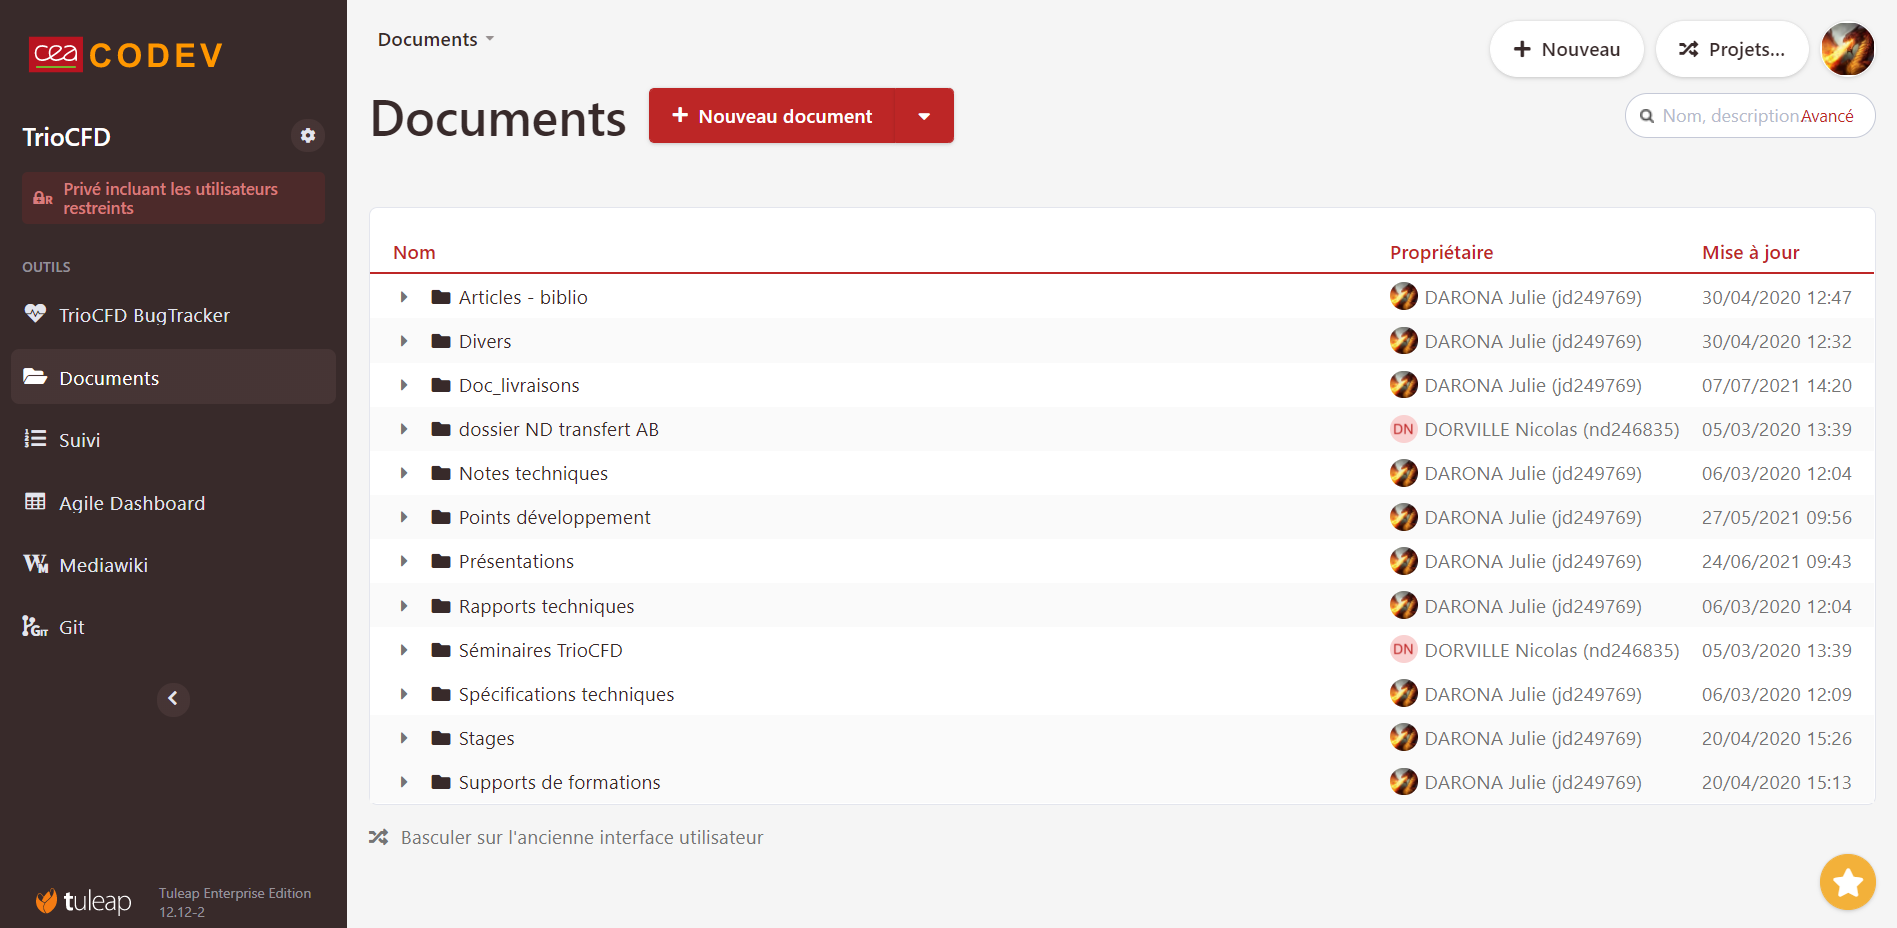
\includegraphics[width=7cm]{pictures/tuleap_documents.png}
   \captionof{figure}{\label{figure:tuleap_doc}Structure de la base documentaire sur TULEAP}
   \end{center}
   \end{multicols}
   \item \textbf{Agile Dashboard} : outil de planification des int\'egrations en vue des livraisons du code. Cet outil a commenc\'e \`a \^etre mis en place \`a partir de la version v1.8.1 (juin 2020). Son utilisation n'est pas encore optimale mais monte progressivement en puissance.
   \item \textbf{MediaWiki} : outil d'aide \`a destination des d\'eveloppeurs pour l'installation de leur environnement de travail
   \newpage
   \item \textbf{Git} : le syst\`eme de contr\^ole des versions sous base GIT est heberg\'e sous TULEAP et est accessible ici. On y trouve  l'adresse du d\'ep\^ot n\'ecessaire pour faire le clonage (voir figure \ref{figure:tuleap_clone}). Aucune action GIT ne doit \^etre lanc\'ee depuis TULEAP car source de nombreuses erreurs. Seules les Pull Request sont effectu\'ees depuis TULEAP en choisissant, dans les menus d\'eroulants, d'une part la branche voulant \^etre int\'egr\'ee et d'autre part, la branche recevant l'int\'egration (voir figure \ref{figure:tuleap_PR}).
   \begin{multicols}{2}
   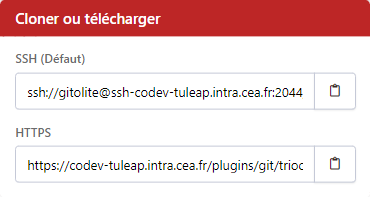
\includegraphics[width=7cm]{pictures/Tuleap_clone.png}
   \captionof{figure}{\label{figure:tuleap_clone}R\'ecup\'eration de l'adresse du d\'ep\^ot GIT via TULEAP}
   \columnbreak
   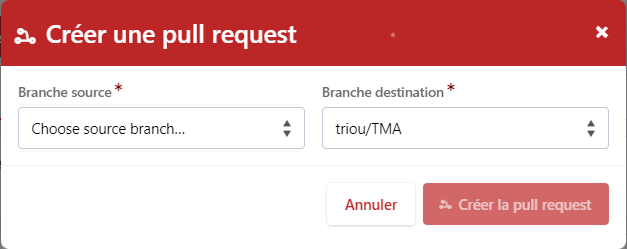
\includegraphics[width=7cm]{pictures/PR.png}\vspace*{1.1cm}
   \captionof{figure}{\label{figure:tuleap_PR}Création d'une Pull Request depuis Tuleap}
   \end{multicols}
\end{itemize}

Nous allons maintenant d\'etailler la partie BugTracker du projet TULEAP de TrioCFD.
\subsection{Fonctionnement g\'en\'eral du BugTracker informatique}
Le BugTracker informatique est utilisé autant par l'\'equipe de TMA que par les agents CEA. A chaque action concernant le code, une fiche spécifique est créée (fiche de Demande d'Intervention). Les fiches répertoriées sur le BugTracker peuvent \^etre trait\'ees soit par l'équipe TMA soit par l'équipe CEA suivant la nature de la fiche. La répartition du traitement des fiches est gérée par le Responsable de Code via le champs \texttt{Way of treatment} de chaque fiche.\\

Pour les demandes re\c cues sur les adresses \'electroniques du projet (voir Chapitre \ref{chapitre:messagerie}), les fiches sont exclusivement ouvertes par l'\'equipe TMA. En revanche, pour les fiches attribu\'ees \`a l'\'equipe CEA, celles-ci sont ouvertes soit directement par un membre de l'\'equipe soit par le responsable de code.\\

Afin de garantir une bonne traçabilité, chaque action de modification, correction ou évolution faite dans le code nécessite l'ouverture au préalable, d'une fiche de Demande d'Intervention. A chaque fiche d'intervention, correspond une branche de développement spécifique dans le gestionnaire de versions dont le nom inclut l'identifiant de la fiche. Ainsi, à tout moment, il est possible de connaître la raison du mouvement des sources du code mais également de connaître l'influence de ce mouvement sur la validation. Nous reviendrons, par la suite, plus en détails sur ces aspects de traçabilité.\\

\subsection{\label{subsec: ficheDI}Constitution d'une fiche de demande d'intervention}
Une fiche de demande d'intervention est constituée de multiples champs. Tous ne sont pas syst\'ematiquement d\'efinis mais les champs vivement recommandés sont détaillés ci-après :\\
\begin{itemize}[label=$\Rightarrow$, font=\LARGE]
   \item \textbf{liste\_diffusion} (\textit{type :} liste ouverte avec lien vers les membres du projet) : permet de retrouver, dans l'annuaire du BugTracker, les personnes potentiellement intéressées/concernées par la fiche. Toute personne identifiée dans ce champ recevra un e-mail automatique du BugTracker la renseignant sur les modifications apportées dans la fiche.
   \item \textbf{Summary} (\textit{type :} chaîne de caractère - \textbf{champ obligatoire}) : correspond au titre de la Demande d'Intervention. Celui-ci doit être court tout en identifiant clairement le problème constaté.  
   \item \textbf{Original Submission} (\textit{type :} Texte) : décrit en détails le problème rencontré ou le développement prévu. Comme, il s'agit d'un champ sans restriction, il est recommandé de donner le maximum d'informations sur le contexte de la fiche et les attendus.
   \item \textbf{Priority} (\textit{type :} liste de choix) : définit la priorité de la fiche considérée par rapport aux autres ouvertes. Ce champ est principalement à destination de l'équipe TMA afin qu'elle soit renseignée sur la priorité de traitement des fiches en fonction des contraintes projet. L'affectation a une priorité induit un délai de résolution : 1-High -> 10 jours ouvrés ; 2-Medium -> 22 jours ouvrés ; 3-Low -> avant la prochaine livraison de version. Le compteur débute à la date renseignée dans le champs \textit{Date hiérarchisation}.
   \item \textbf{Category} (\textit{type :} liste de choix) : correspond à une des catégories de Demandes d'Intervention listées au Chapitre \ref{chapitre:termes} et identifiées dans le contrat de marché de la TMA.
   \item \textbf{Sub project associated} (\textit{type :} liste de choix) : permet d'identifier le Baltik impacté par la DI.
   \item \textbf{Authorization to work on this} (\textit{type :} case à cocher) : champ destiné à la TMA pour lui donner l'autorisation de débuter les travaux sur la DI.
   \item \textbf{Date hiérarchisation} (\textit{type :} date) : champ à mettre à jour avec le champ précédent (Authorization to work on this) et à renseigner avec la date du jour du lancement des travaux sur la DI. Cette date permettra de vérifier que le délai de réalisation de la DI est bien tenu.
   \item \textbf{Status} (\textit{type :} liste de choix) : correspond à l'état de vie de la fiche. Cette notion sera plus approfondie dans la section suivante (voir section \ref{sec:etatsDI}). 
   \item \textbf{Assigned to} (\textit{type :} liste à choix multiples avec lien vers les membres du projet) : correspond à(aux) membre(s) du projet travaillant sur le traitement de la DI.
   \item \textbf{Way of treatment} (\textit{type :} liste de choix) : 2 choix sont possibles ; soit la demande est traitée par le CEA (\textit{ResolutionByCEA}) soit par la TMA (\textit{ResolutionByTMA}).
   \item \textbf{Work load} (\textit{type :} flottant) : champ renseigné uniquement lorsque la DI est traitée par l'équipe TMA afin de s'assurer que la charge de traitement n'a pas été trop conséquente et a bien respecté les indicateurs contractuels.
\end{itemize}

%\begin{multicols}{2}
\begin{minipage}[c]{0.35\linewidth}

\vspace*{0.2cm}
Ainsi, l'aspect général de la fiche au moment de sa création est visualisable ci-contre (voir Figure \ref{figure:fiche_DI})
\\
Tous les champs ne sont pas obligatoires à la création de la fiche mais peuvent le devenir en fonction de son état de traitement. De même, tous les champs sont modifiables à tout moment. Ainsi, on veillera à mettre à jour le titre de la fiche si, lors de son traitement, on constate que le problème avait été initialement mal identifié.\\
\\
\\
La gestion du BugTracker Tuleap est du ressort du Responsable de Code. En fonction de l'évolution des besoins, des adaptations de ces champs pourront ponctuellement être faites.
\\
\\
\end{minipage} \hfill
\begin{minipage}[c]{0.6\linewidth}
   
   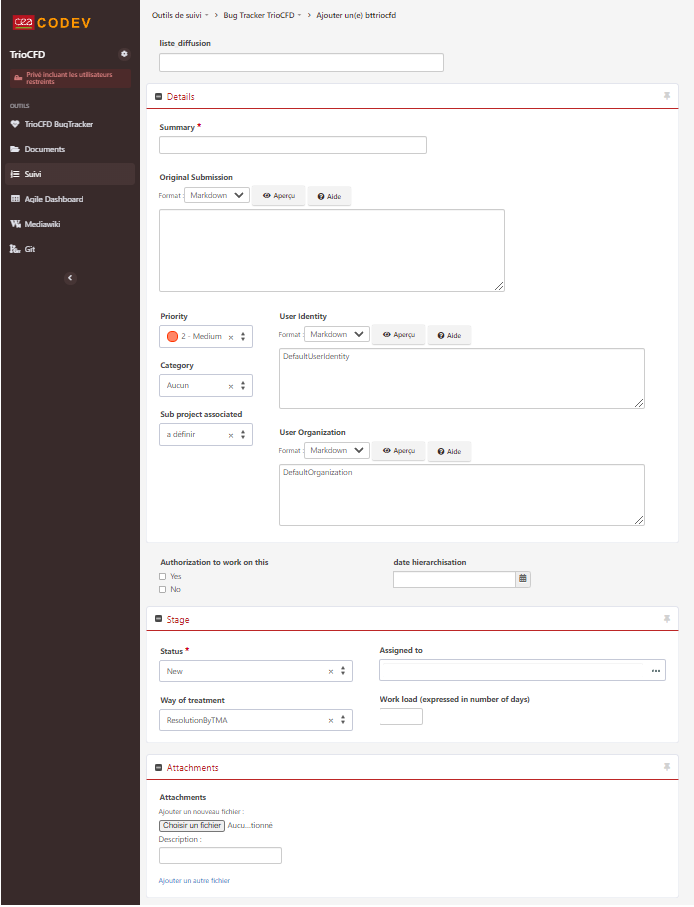
\includegraphics[width=9.5cm]{pictures/Fiche_DI.png}\vspace*{0.2cm}
   \captionof{figure}{\label{figure:fiche_DI}Champs à renseigner pour la création d'une Demande d'Intervention TrioCFD}
%\end{multicols}
\end{minipage}

Une fois la fiche de DI créée, celle-ci est répertoriée dans le BugTracker avec un identifiant unique à 6 chiffres qui servira à nommer la branche GIT associée. On observera sur la figure \ref{figure:tracker_overview}, cet identifiant dans la $1^{ère}$ colonne du tableau.\\ \vspace*{0.3cm}

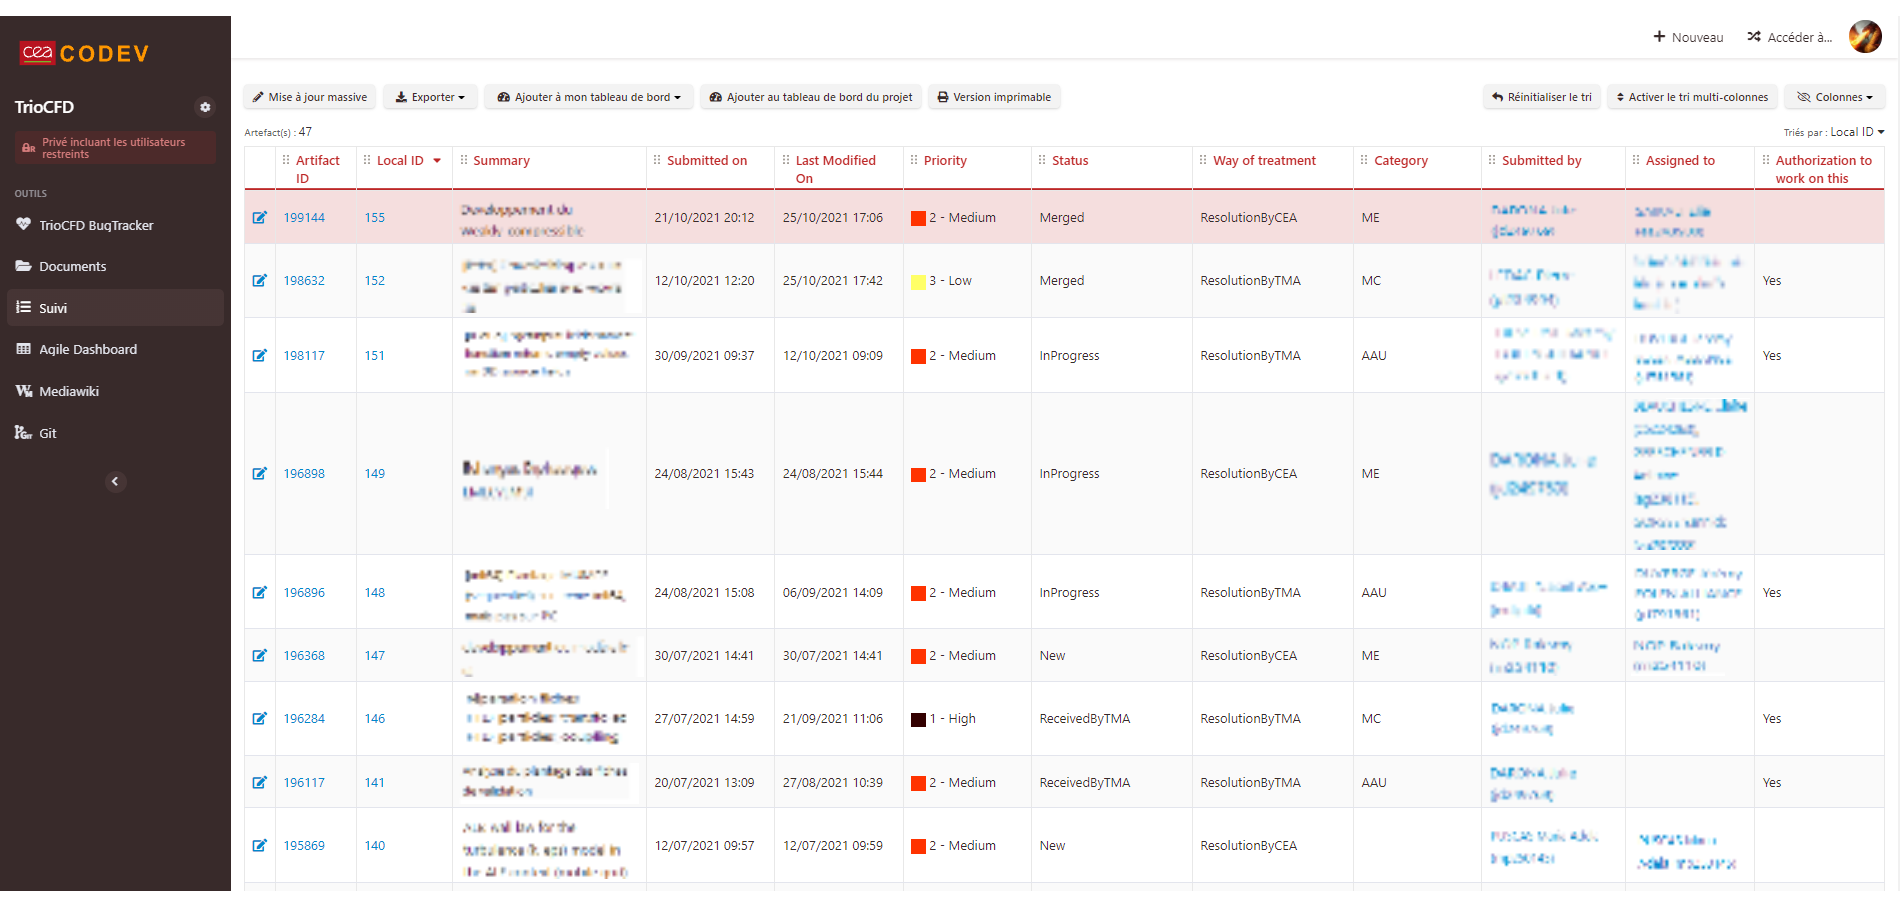
\includegraphics[width=16cm]{pictures/tracker_overview.png}\vspace*{0.1cm}
\captionof{figure}{\label{figure:tracker_overview} Vue générale du BugTracker TrioCFD et de quelques fiches de Demandes D'Intervention en cours}
\vspace*{0.3cm}
La vue générale de la figure \ref{figure:tracker_overview} permet d'avoir rapidement la visualisation des fiches ouvertes, leur priorité, leur état d'avancement et les personnes en charge de leur résolution. Cette vue peut être ajustée en fonction des besoins de suivi et ses différentes configurations, conservées.

\subsection{\label{sec:etatsDI}États de traitement d'une fiche de Demande d'Intervention }
Une fiche de DI du BugTracker TrioCFD suit un processus de traitement clairement défini et a, suivant son état, un statut particulier défini dans le champ \texttt{Status}. Ce cycle de vie est illustré par la figure \ref{figure:workflow_Trio}. Il est composé de 6 états (dans les boites rectangulaires) qui sont :\newline
\begin{itemize}[label=$\Rightarrow$, font=\LARGE]
   \item \textbf{NEW} : pour une DI saisie directement par l'utilisateur (agent CEA), une fois les champs précisés au paragraphe précédent, remplis et la création de la fiche validée, celle-ci passe automatique en statut NEW.
   \item \textbf{RECEIVED BY TMA} : (pour une DI créée par l'équipe TMA) une fois les champs précisés au paragraphe précédent remplis et la création de la fiche validée, la TMA la définit en statut RECEIVED BY TMA. Il en est de même pour les DI en statut NEW lorsque son traitement est du ressort de la TMA. Cet état signifie que la TMA a menée une première analyse de la demande et a commencé à identifier l'origine du problème. Ces premiers résultats d'analyse seront discutés lors de la réunion hebdomadaire entre le RPL et le RML. Il sera alors décidé de la pertinence de cette demande, de sa priorité de traitement (champ \texttt{Priority)} et du lancement ou non des travaux sur celle-ci (champ \textit{Authorization to work on this}).
   \item \textbf{IN PROGRESS} : lorsque le traitement d'une fiche débute, il appartient à la personne en charge de son traitement de la passer en statut IN PROGRESS. Ce changement de statut nécessite de renseigner le champ \texttt{Assigned to} afin qu'il soit pris en compte. Cet état permet de savoir que les travaux ont débuté sur le sujet. C'est dans ce statut que la DI passera la plus grande partie de sa vie. Lorsque le travail sera achevé, si la DI nécessite une modification du code source, une Pull Request (voir figure \ref{figure:tuleap_PR}) sera effectuée par la personne ayant traitée la DI.
   \item \textbf{MERGED} : une fois la branche correspondante à la DI intégrée dans la branche de développement du code (branche \texttt{triou/TMA}) par l'Intégrateur, celui-ci la passe en statut MERGED. L'équipe de TMA aura ainsi connaissance des intégrations d'un jour sur l'autre et prêtera une attention toute particulière au retour hebdomadaire de l'atelier de Vérification. En cas d'impacts non attendus sur la base de vérification, la DI est repassée en statut IN PROGRESS afin d'investiguer sur ces écarts imprévus et les justifier ou apporter des correctifs pour les résorber. Ce statut concerne uniquement les DI de type MC (Maintenance Corrective) ou de type ME (Maintenance Évolutive). 
   \item \textbf{TREATED/RESOLVED} : cet état signifie que l'ensemble des travaux nécessaires pour mener à bien le traitement de la fiche ont été faits. Dans le cas d'une ME ou d'une MC, ce statut est atteint lorsque la branche de travail a été intégrée avec succès dans la branche en développement du code et que les éventuels impacts ont été validés. Pour une fiche de type AAU, l'initiateur de la demande a retourné un avis positif sur la solution proposée pour résoudre son problème.
   \item \textbf{CLOSED} : le travail réalisé dans le cadre de cette Demande d'Intervention est validé par le RPL (demandes en traitement TMA) ou par le Responsable de Code (demandes en traitement CEA). Une fois cet état atteint, plus aucun travail ne doit être mené sur la demande. Si d'aventure, d'avantage de travail était identifié à posteriori, une nouvelle fiche devra alors être créée. 
\end{itemize}
\vspace*{0.5cm}
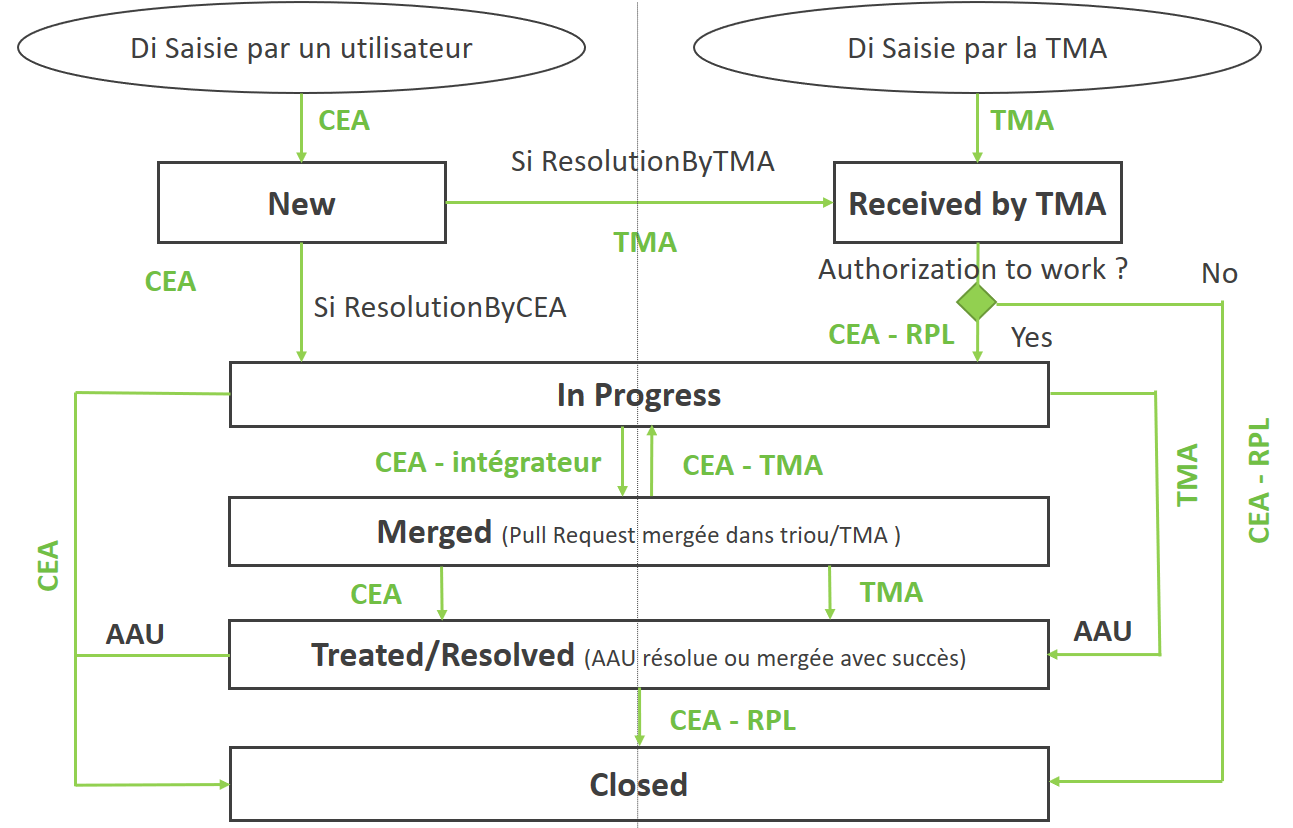
\includegraphics[width=16cm]{pictures/workflow_Trio.png}\vspace*{0.1cm}
\captionof{figure}{\label{figure:workflow_Trio} Workflow du BugTracker TrioCFD}
\vspace*{1.5cm}
L'ensemble de cette démarche est également expliquée dans le MediaWiki du BugTracker TrioCFD. \\
\\ Le respect de ces procédures garantit une bonne tra\c cabilité de l'ensemble des actions relatives au code mais également de toute modification apportée dans les sources. Le Responsable de Code a donc pour mission des les expliquer et de veiller à leur bonne application. En cas de non respect, il a à sa charge d'apporter les modifications nécessaires afin de rétablir leur bon déroulement (saisie des fiches de DI, rappel à l'ordre, blocage provisoire des droits d'intégration,...).

\newpage
\chapter{Suivi et archivage des études}
\lhead{Suivi et archivage des études}
\rhead{OUTILS}
Pour le suivi et l'archivage des études menées sous TrioCFD, le code dispose d'un Tracker propre sous Tuleap dans le projet Etudes-STMF à l'adresse : \url{https://codev-tuleap.intra.cea.fr/projects/etudes-stmf/}. D'autres codes du service sont également hébergés sous ce projet Tuleap mais chacun d'eux dispose de son propre Tracker. Si quelques adaptations sont nécessaires d'un code à l'autre pour répondre au mieux à leurs besoins, ils restent néanmoins très proches afin d'en faciliter la consultation. Ce projet a été mis en place début 2019 et est rentré en production mi 2019. Le Tracker de chacun des codes permet d'assurer un suivi de chacune des études menées sur le code concerné. Il n'est en aucun cas un lieu d'archivage des études. Pour l'archivage, un espace dédié a été créé sur le nouveau système de stockage Linux du service nommé TITANIA. Le lien avec cet espace de stockage ainsi que sa structure seront détaillés dans la dernière section de ce chapitre.
\subsection{Objectifs du suivi et de l'archivage des études}
Avant la création de ce système, aucun outil n'était proposé pour conserver une mémoire de l'ensemble des études menées sur un code. Chacun conservait, en local sur son poste de travail, les études qu'il avait réalisées. Or cette méthodologie de travail présente de forts inconvénients et risques parmi lesquels, on peut citer : 
\begin{itemize}
   \item Pertes scientifiques très conséquentes en cas de départ de la personne ayant réalisé des études sur un code ou en cas de changement de localisation des activités
   \item Pas de "mémoire" des codes sur les études pour lesquelles ils ont été utilisés
   \item Anciennes études inexploitables au fur à mesure que le temps passe
   \item Incapacité de reproductibilité des dossiers de sureté
   \item Limitations de la mutualisation des connaissances (échanges sur les pistes suivies ayant abouti ou non à la résolution des problèmes, avis des développeurs pouvant aider la partie étude,…)
   \item Benchmark entre les différents codes peu nombreux
   \item Couplage entre les différents codes peu nombreux
   \item Doublement d'études en cas de manque de dialogue entre les projets ou les laboratoires
   \item Pas de réelle vision d'ensemble de la multitude des actions menées dans le service
\end{itemize}
Les objectifs de ce suivi sont donc de limiter autant que possible les problèmes identifiés précédemment.

\subsection{Constitution d'une fiche de Suivi d'Etude}
Comme les fiches de Demande d'Intervention, les fiches de Suivi d'Etude contiennent plusieurs champs. Ils sont moins nombreux que ceux d'une Demande d'Intervention informatique car ce Tracker ne s'adresse pas au même public et son utilisation se doit d'être plus simple.  Une fiche de Suivi d'Etude est constituée de plusieurs rubriques, chacune étant constituée de différents champs. L'ensemble de cette structure est détaillée ci-dessous.\\
\begin{minipage}[c]{0.45\linewidth}
\textbf{Général}

\begin{itemize}[label=$\Rightarrow$, font=\LARGE]
   \item \textbf{Titre de l'étude} (\textit{type :} chaîne de caractères - \textbf{champ obligatoire}) : correspond au titre de l'étude menée. Celui-ci doit être relativement court tout en relatant sans ambiguïté le ou les domaine(s) traité(s) dans l'étude
   \item \textbf{Description} (\textit{type :} texte - \textbf{champ obligatoire}) : décrit, en détails, l'étude qui va être menée avec notamment ses objectifs, les phénomènes observés, les moyens utilisés pour valider l'étude,...
   \item \textbf{Mots-clés} (\textit{type :} chaîne de caractères) : à renseigner de quelques mots clés bien choisis afin de retrouver plus rapidement les études traitant d'un sujet spécifique
\end{itemize}

\end{minipage} \hfill
\begin{minipage}[c]{0.5\linewidth}
   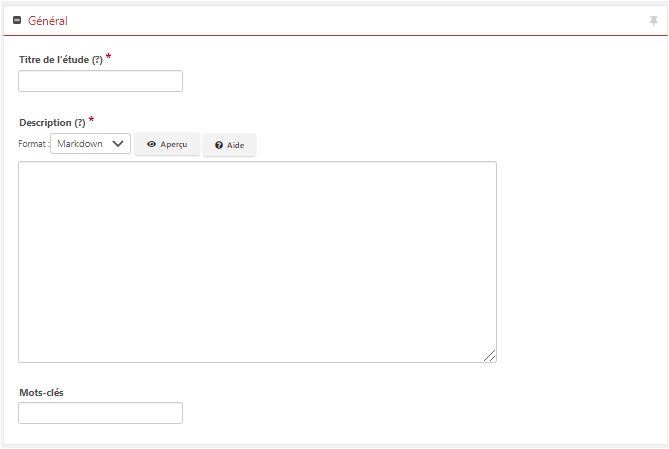
\includegraphics[width=9cm,trim = 0 0 100 0 , clip = true]{pictures/GEA-general.png}\vspace*{0.2cm}
   \captionof{figure}{\label{figure:GEA-general}Constitution d'une fiche de Suivi d'Etude - partie générale}

\end{minipage}

\vspace{0.5cm}

\begin{minipage}[c]{0.45\linewidth}
\textbf{Contexte}
\begin{itemize}[label=$\Rightarrow$, font=\LARGE]
   \item \textbf{Projet} (\textit{type :} liste de choix) : à renseigner si l'étude est réalisée dans le cadre du financement par un projet
   \item \textbf{Lot/application} (\textit{type :} liste de choix) : spécifie le lot du projet si le champ précédent a été renseigné
   \item \textbf{Accords de confidentialité} (\textit{type :} liste de caractères) : renseigne si l'étude est soumise à des accords de confidentialité et dans quel cadre d'accord
   \item \textbf{Partenariat} (\textit{type :} liste de caractères) : permet de préciser si l'étude a été réalisée en partenariat avec une autre entité (laboratoire, université, partenaire industriel,...)
   \item \textbf{Jalon} (\textit{type :} bouton radio - \textbf{champ obligatoire}) : définit si l'étude constitue un jalon pour un projet
   \item \textbf{Livrable} (\textit{type :} liste de choix - \textbf{champ obligatoire}) : définit si un livrable doit être émis suite à l'étude
   \item \textbf{DR} (\textit{type :} liste de choix - \textbf{champ obligatoire}) : renseigne si l'étude est soumise à une règle restreinte de diffusion
\end{itemize}

\end{minipage} \hfill
\begin{minipage}[c]{0.5\linewidth}
   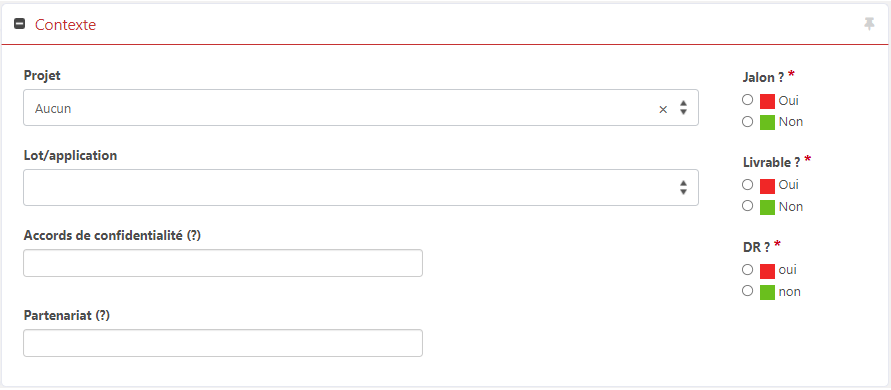
\includegraphics[width=9cm]{pictures/GEA-contexte.png}\vspace*{0.2cm}
   \captionof{figure}{\label{figure:GEA-contexte}Constitution d'une fiche de Suivi d'Etude - partie contexte}

\end{minipage}

\vspace{0.5cm}
\textbf{Informations sur l'étude}
\begin{itemize}[label=$\Rightarrow$, font=\LARGE]
   \item \textbf{Autre personne potentiellement intéressée} (\textit{type :} liste ouverte avec lien vers les membres du projet) : permet de retrouver dans l'annuaire du Tracker, les personnes potentiellement intéressées/concernées par la fiche. Toute personne stipulée dans ce champ recevra un e-mail automatique du BugTracker la renseignant sur les modifications apportées dans la fiche.
   \item \textbf{Catégorie} (\textit{type :} case à cocher) : permet d'identifier si il s'agit d'une nouvelle étude, de la reprise d'une étude,...
\end{itemize}

\begin{minipage}[c]{0.45\linewidth}
\begin{itemize}[label=$\Rightarrow$, font=\LARGE]
   \item \textbf{Version} (\textit{type :} liste de choix) : renseigne sur la version du code utilisée pour mener l'étude. Les différentes versions livrées depuis la v1.7.9 sont disponibles dans le menu déroulant ainsi que la version de développement. Si l'étude était menée sur la version de développement, il est indispensable de renseigner le champ suivant.
   \item \textbf{Préciser SHAI-ID si version développement ou autre version} (\textit{type :} chaîne de caractères) : correspond au "code barre" ou SHA1 ID sous le gestionnaire de configuration GIT, de la version de développement utilisée pour mener l'étude.
\end{itemize}

\end{minipage} \hfill
\begin{minipage}[c]{0.5\linewidth}
   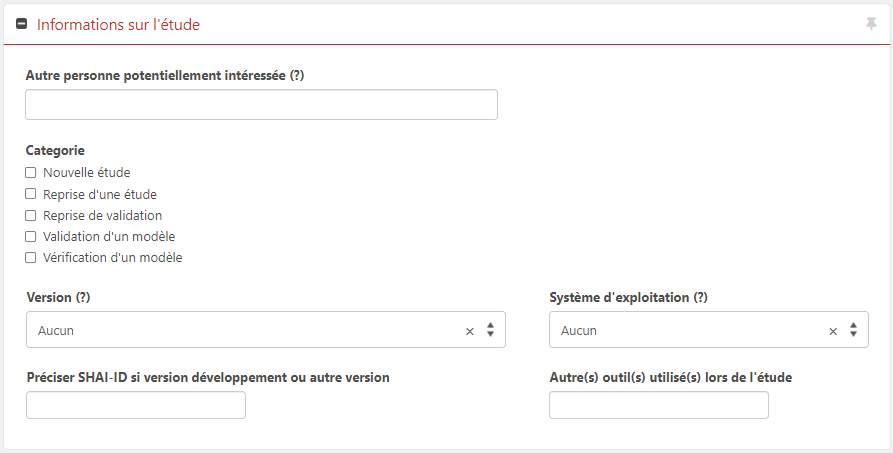
\includegraphics[width=9cm]{pictures/GEA-info.png}\vspace*{0.2cm}
   \captionof{figure}{\label{figure:GEA-info}Constitution d'une fiche de Suivi d'Etude - partie informations sur l'étude}

\end{minipage}

\begin{itemize}[label=$\Rightarrow$, font=\LARGE]
   \item \textbf{Système d'exploitation} (\textit{type :} liste de choix) : renseigne sous quel système d'exploitation l'étude a été menée. En effet, on peut parfois observer de petits écarts de portabilité entre les machines. Si l'étude archivée était amenée à être reprise ou en cas d'inspection des Autorités de Sureté, cette information est capitale.
   \item \textbf{Autre(s) outil(s) utilisé(s) lors de l'étude} (\textit{type :} chaîne de caractères) : si d'autres outils ont été utilisés dans le cadre de l'étude (\textit{eg} SHAPER pour la construction de la CAO, SALOME pour l'établissement du maillage), le ou les outil(s) ainsi que leur version sont à renseigner ici.
\end{itemize}

\vspace{0.5cm}

\begin{minipage}[c]{0.45\linewidth}
\textbf{Avancement}
\begin{itemize}[label=$\Rightarrow$, font=\LARGE]
   \item \textbf{Etat d'avancement} (\textit{type :} liste de choix - \textbf{champs obligatoire}) :  correspond à l'état de vie de la fiche. Cette notion sera plus approfondie dans la section suivante. 
   \item \textbf{Traité par} (\textit{type :} liste à choix multiple avec lien vers les membres du projet) : correspond à(aux) membre(s) du projet travaillant sur le traitement de la DI.
\end{itemize}

\end{minipage} \hfill
\begin{minipage}[c]{0.5\linewidth}
   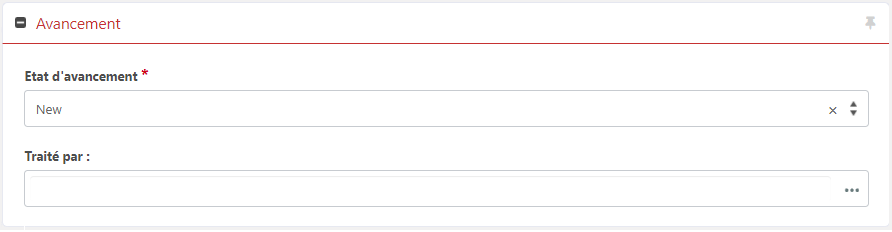
\includegraphics[width=9cm]{pictures/GEA-avancement.png}\vspace*{0.2cm}
   \captionof{figure}{\label{figure:GEA-avancement}Constitution d'une fiche de Suivi d'Etude - partie avancement de l'étude}

\end{minipage}

\vspace{0.5cm}

\textbf{Finalisation de l'étude}\\
Cette partie est à renseigner lorsque l'étude est terminée.
\begin{itemize}[label=$\Rightarrow$, font=\LARGE]
   \item \textbf{Données finales sauvegardées sur Titania} (\textit{type :} cases à cocher) :  correspond à la liste des données qui auront été sauvegardées sur Titania. Ainsi, à la consultation d'une fiche, l'utilisateur saura immédiatement quelles données pourront être accessibles rapidement puisque sauvegardées sur le système d'archivage des études.
   \item \textbf{Autres données sauvegardées sur Titania} (\textit{type :} chaîne de caractères) : si d'autres données ont été sauvegardées sur Titania mais ne correspondent pas aux catégories proposées dans le champ précédent, elles peuvent être renseignées manuellement dans celui-ci.
\end{itemize}
\begin{minipage}[c]{0.45\linewidth}

\begin{itemize}[label=$\Rightarrow$, font=\LARGE]
   \item \textbf{Référence note émise} (\textit{type :} chaîne de caractères) : si dans le cadre de cette étude, une note a été émise, il est possible d'en renseigner son numéro d'émission ici afin de la retrouver plus rapidement dans la base documentaire de notes du département.
   \item \textbf{Temps passé (jours)} (\textit{type :} chaîne de caractères) : peut être rempli pour donner un retour d'expérience sur le temps nécessaire pour traiter chaque catégorie d'étude et faciliter les chiffrages postérieurs.
\end{itemize}

\end{minipage} \hfill
\begin{minipage}[c]{0.5\linewidth}
   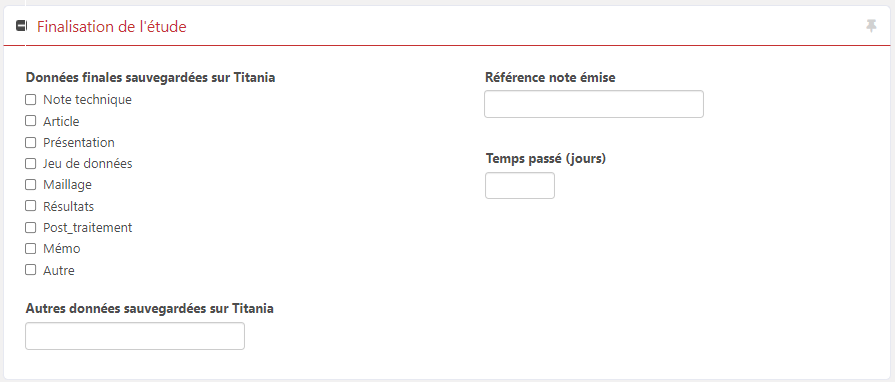
\includegraphics[width=9cm]{pictures/GEA-finalisation.png}\vspace*{0.2cm}
   \captionof{figure}{\label{figure:GEA-finalisation}Constitution d'une fiche de Suivi d'Etude - partie finalisation de l'étude}

\end{minipage}

\vspace{0.5cm}

\begin{minipage}[c]{0.45\linewidth}
\textbf{Pièces jointes}\\
Des données légères peuvent être sauvegardées ici mais il ne s'agit, en aucun cas du lieu d'archivage de l'étude. Tuleap n'est pas conçu pour supporter de gros volumes de données et au delà de 50 Go de données stockées, son temps de réponse devient très important, nuisant fortement à son utilisation. Ainsi, seules des données de petites tailles (\textit{eg} échanges de mail, supports de présentation,...) peuvent être sauvegardées ici. Ces données correspondent plutôt à des données nécessaires lors de l'étude et devront ensuite être sauvegardées sur le système d'archivage.\\
\end{minipage} \hfill
\begin{minipage}[c]{0.5\linewidth}
   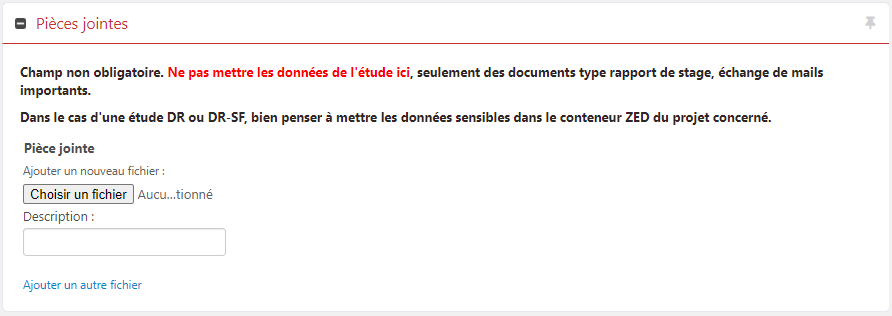
\includegraphics[width=9cm]{pictures/GEA-PJ.png}\vspace*{0.2cm}
   \captionof{figure}{\label{figure:GEA-PJ}Constitution d'une fiche de Suivi d'Etude - partie pièces jointes}

\end{minipage}

D'autre part, en cas d'une étude contenant des données sensibles (type Diffusion Restreinte ou Diffusion Restreinte - Spéciale France), ces données ne devront pas figurer "en clair" dans la fiche de Suivi de l'Etude. Elles devront avoir été préalablement placées dans le conteneur du projet hébergeant l'étude. C'est ce conteneur qui sera ensuite sauvegardé en pièce jointe dans la fiche.

\vspace{0.5cm}

\begin{minipage}[c]{0.45\linewidth}
\textbf{Permissions}\\
Le dernier champ a remplir avant la finalisation de la fiche de Suivi d'Etude concerne les droits d'accès à celle-ci. Ce champ est \textbf{obligatoire}. Si il s'agit d'une étude contenant des données sensibles (type Diffusion Restreinte ou Diffusion Restreinte - Spéciale France), il faudra veiller à sélectionner uniquement le groupe DRSF-STMF. Seul ce groupe-là pourra alors voir les études de ce type. Pour les autres études n'ayant aucune donnée sensible, le groupe Permanents-STMF sera à sélectionner ainsi que le groupe temporaires-STMF si on souhaite mettre la fiche à disposition des personnes n'étant pas en contrat permanents (stagiaires, doctorants, post-doc, CDD,...). \\
\end{minipage} \hfill
\begin{minipage}[c]{0.5\linewidth}
   \begin{figure}[H]
      \centering
      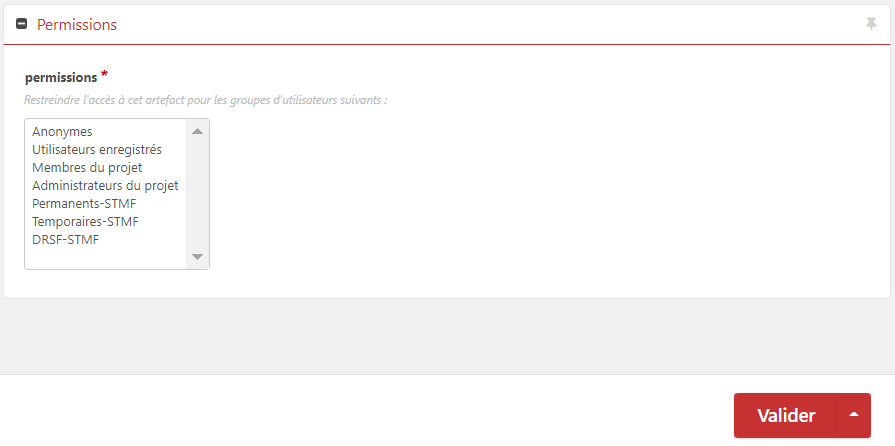
\includegraphics[width=9cm]{pictures/GEA-permissions.png}
      \vspace*{0.2cm}
      \captionof{figure}{\label{figure:GEA-permissions}Constitution d'une fiche de Suivi d'Etude - partie permissions}
   \end{figure}
\end{minipage}

Lorsque tous les champs ont bien été remplis, veillez à bien appuyer sur le bouton \texttt{Valider} afin de générer la création de la fiche. L'ensemble des champs peut être modifié après la création de la fiche.

\vspace{0.5cm}

\begin{minipage}[c]{0.5\linewidth}
   \begin{figure}[H]
      \centering
      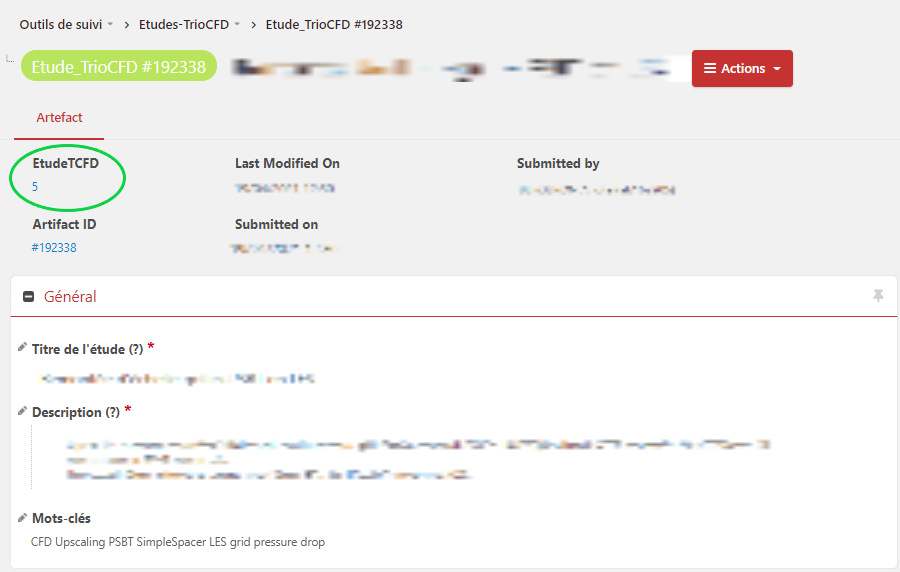
\includegraphics[width=8cm]{pictures/GEA-identification.png}
      \vspace*{0.2cm}
      \captionof{figure}{\label{figure:GEA-identification}Constitution d'une fiche de Suivi d'Etude - numéro d'identification de la fiche}
   \end{figure}
\end{minipage} \hfill
\begin{minipage}[c]{0.45\linewidth}
Une fois la fiche créée, elle dispose alors d'un identifiant unique (voir encadré vert sur figure ci-contre). Cet identifiant servira à nommer le répertoire de sauvegarde de l'étude afin de le retrouver immédiatement sur le système d'archivage sous Titania.

\end{minipage}


\subsection{États de traitement d'une fiche de suivi d'étude}

Contrairement au BugTracker informatique, le gestionnaire de suivi des études comporte un Worflow beaucoup plus simple avec seulement 4 états pour une fiche de Suivi d'Etude. Ces 4 états sont les suivants :
\begin{itemize}[label=$\Rightarrow$, font=\LARGE]
   \item \textbf{NEW} : à la création de la fiche de Suivi d'Etude, celle-ci est automatiquement en statut NEW. L'étude a été identifiée mais le travail dessus n'a pas encore été amorcé.
   \item \textbf{IN PROGRESS} : dès que le travail est amorcé, la personne en charge de l'étude passe la fiche de suivi correspondante à l'état IN PROGRESS. Pour le passage dans ce statut, il est nécessaire de renseigner le champ \texttt{Traité par}. En effet, à ce stade, il y a nécessairement une personne qui a été identifiée pour mener à bien cette étude. La fiche de Suivi de l'Etude va passer la majorité de sa vie dans cet état.
   \item \textbf{SAVED} : une fois l'étude, à proprement parler, terminée, les données nécessaires à sa reproduction ou reprise doivent être archivée sur le système d'archivage sous Titania. Une fois que cet archivage est fait, la fiche passe alors en statut SAVED. Pour ce passage, 2 champs de la fiche doivent avoir été au préalablement remplis à savoir \texttt{Données sauvegardées sur Titania} et \texttt{Version}. Ce dernier champ est, en effet, absolument nécessaire pour que les données archivées puissent être ré-exploitées. Un jeu de données peut différer d'une version à l'autre du code mais également être fonctionnel sur des versions antérieures et, nécessiter une mise à jour pour qu'il le soit sur une nouvelle version.
   \item \textbf{CLOSED} : une fois l'étude menée et les documents associés archivés, la fiche de suivi peut alors être clôturée.
\end{itemize}

Il s'agit là du déroulé le plus standard d'une fiche d'étude. Il est toutefois possible qu'il y ait plusieurs itérations avant qu'une fiche ne soit clôturée. La figure \ref{figure:worflow-etude} représente l'ensemble du Worflow et récapitule les champs nécessaires pour le passage d'un statut à l'autre.\\
\vspace{0.1cm}
\begin{figure}[H]
   \centering
   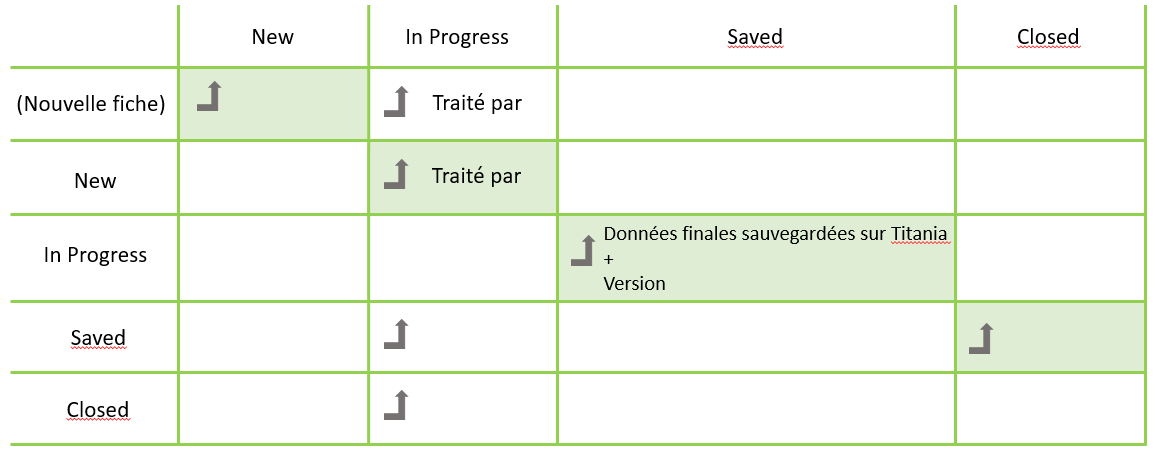
\includegraphics[width=13cm]{pictures/worflow-etude.png}                        
   \vspace*{0.2cm}
   \captionof{figure}{\label{figure:worflow-etude}Worflow du gestionnaire de suivi des études de TrioCFD}
\end{figure}
\subsection{Archivage des études}
Avant de passer dans l'état SAVED décrit au paragraphe précédent, toutes les données nécessaires à la reprise de l'étude doivent avoir été archivée sur Titania. Cette méthodologie d'archivage va être décrite dans cette section.\\

Le système d'archivage Linux est présent sur le nouveau système Linux du DM2S nommé Titania. Il est accessible autant depuis Linux que depuis Windows. Celui-ci s'appelle etudes-stmf (même nom que le projet sur Tuleap, moyennant la casse). L'accès à l'espace de stockage via LINUX se fait à partir d'un poste connecté à Titania. L'espace est ensuite accessible sur /home/etudes-stmf :
\begin{lstlisting}
> cd /home/etudes-stmf 
\end{lstlisting}
On trouve ici les répertoires des différents codes participant au projet, donc TrioCFD, et présents sur le gestionnaire d'études dans Tuelap.\\
Pour avoir accès à l'espace d'archivage via Windows, il suffit d'ouvrir un explorateur de fichier et de saisir l'adresse suivante dans la barre d'accès en haut de la fenêtre :
\begin{lstlisting}
\\titania\home_projet\partage/etudes-stmf
\end{lstlisting}
Il est conseillé de connecter un lecteur sur cet emplacement afin de ne pas avoir à le rechercher à chaque fois. Comme sur Linux, vous aurez alors accès aux répertoires des différents codes participant au projet et présents sur le gestionnaire d'études dans Tuleap (voir figure \ref{figure:Sauvegarde-Titania}).\\
Sous chacun des répertoires des codes, autant de répertoires que de fiches de Suivi d'Etude présentes sur Tuleap devront être créés. A un répertoire correspond les données d'une fiche d'étude. Le lien entre la fiche étude sous Tuleap et le répertoire d'archivage sur Linux se fera via le nom donné au répertoire sur le système d'archivage qui correspondra au numéro de l'étude généré par Tuleap. Chaque répertoire d'étude est composé de plusieurs sous-dossiers avec une structure identique pour chaque étude :
\begin{itemize}[label=$\Rightarrow$, font=\LARGE]
   \item \textbf{01-MEMO} : un ou plusieurs mémos permettant de bien identifier les données qui ont été archivées comme l'organisation des répertoires de calculs ou toute information qui semble utile pour permettre la bonne compréhension et reproductibilité de l'étude.
   \item \textbf{02-Donnees\_Entrees} : ce répertoire a pour but de stocker les données qui ont été nécessaires à la modélisation de l'étude (plans de l'expérience si une comparaison par rapport à l'expérimental a été faite, le jdd d'origine si il s'agit d'une reprise d'étude,...) 
   \item \textbf{03-Calculs} : c'est ici que sont stockés l'ensemble des jdds, maillages, post-traitement et éventuellement les résultats. Il se peut que de nombreux jdds aient été créés pour mener à bien l'étude. Il est recommandé de procéder, tout d'abord à un tri de ces calculs puis de ranger chacun d'entre eux dans un répertoire différent sous 03-Calculs par exemple Calcul01, Calcul02,... (nommage à la discrétion de chacun). Chaque répertoire de calcul contiendra le maillage propre au calcul, le jdd, le fichier de post-traitement et éventuellement, les résultats. Afin de mieux comprendre en quoi consiste chacun de ces répertoires de calcul une fiche mémo pourra être élaborée et sauvegardée dans \texttt{01-MEMO}
   \item \textbf{04-Documents\_Emis} : seront sauvegardés ici tous les documents émis suite à cette étude. Cela pour être un article, une présentation, une note technique,... 
   \item \textbf{05-Verification} : seront sauvegardés dans ce répertoire tous les retours et échanges qui auraient pu y avoir dans le cadre de la vérification de l'étude
   \item \textbf{06-References} : seront sauvegardés ici les articles ou autres références bibliographiques ayant contribué aux réflexions menées durant l'étude
   \item \textbf{07-Codes-scripts} : si des scripts ou des codes non suivis en gestion de configuration (git, github,...) ont été élaborés dans le cadre de l'étude, ils seront stockés dans ce sous-répertoire.
\end{itemize}
\begin{figure}[H]
   \centering
   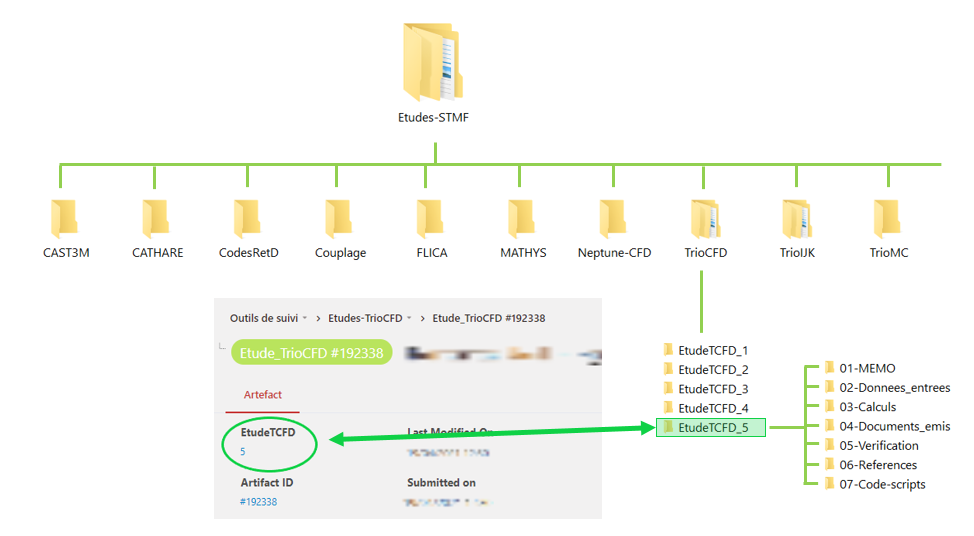
\includegraphics[width=14.5cm]{pictures/Sauvegarde-Titania.png}
   \vspace*{0.2cm}
   \captionof{figure}{\label{figure:Sauvegarde-Titania}Organisation de la sauvegarde des études sous Titania}
\end{figure}
\vspace{0.2cm}
Afin de générer rapidement cette arborescence, un script est présent dans le répertoire de TrioCFD. Celui-ci ce nomme \texttt{gen\_dossier.sh}. Il est alors demandé le numéro de la fiche pour laquelle le dossier doit être créé et l'ensemble est alors automatiquement généré. Son déroulé a lieu de la façon suivante (exemple de la figure \ref{figure:Sauvegarde-Titania}):

\footnotesize
\begin{lstlisting}
 > ./gen_dossier.sh             % lancement script
 Numero de la fiche Tuleap ?    % demande du numero de la fiche Tuleap correspondante
 5                              % numero renseigne par l'utilisateur
 Repertoire EtudeTCFD_5 cree    % message de succes de la creation
\end{lstlisting}
\normalsize
Le remplissage de tous les répertoires présentés ci-dessus n'est, en aucun cas, obligatoire tant que toutes les données indispensables à la compréhension et la reproductibilité de l'étude sont présentes. Si un répertoire est vide, il est demandé de ne pas le supprimer et le laisser vide, en l'état.\\
Pour le stockage des documents, les formats de stockage des données doivent être les plus standard possibles et lisibles par une majorité d'OS à savoir des fichiers texte (jeux de données, post-traitement, scripts, latex,...) ou des fichiers pdf. En cas de  sauvegarde de fichiers à format propriétaire, type Office ou LibreOffice, il est recommandé d'archiver à la fois ce type de fichier mais également leur impression au format pdf.\\
\\
L'ensemble de cette méthodologie pour le suivi et l'archivage d'une étude est détaillé dans le MediaWiki du projet Tuleap Etudes-STMF à l'adresse : \url{https://codev-tuleap.intra.cea.fr/plugins/mediawiki/wiki/etudes-stmf/index.php?title=Accueil}.

\chapter{\label{chapitre:GIT}Outil de gestion de versions (GIT)}
\lhead{Outil de gestion de versions}
\rhead{OUTILS}
Deux ans après le début du développement de la plateforme, celle-ci est passée en gestion de configuration, d'abord sous SCCS, puis sur ClearCase et depuis mi 2013 sur GIT. L'ensemble du code TrioCFD y est stocké que ce soit le code source, les procédures, les fiches de V\&V ou la documentation. Cette base GIT est hébergée par Tuleap et se nomme triocfd-code.\\
\\
\subsection{Définition de la gestion de versions}
Le contrôle de version, également appelé contrôle de source, désigne la pratique consistant à suivre et à gérer les changements apportés au code d'un logiciel. Les systèmes de contrôle de version sont des outils logiciels qui permettent aux équipes de développement de gérer les changements apportés au code source au fil du temps. Les logiciels de contrôle de version gardent une trace de chaque changement apporté au code dans un type spécial de base de données. Si une erreur est commise, les développeurs peuvent revenir en arrière et comparer les versions antérieures du code, ce qui leur permet de corriger l'erreur tout en minimisant les perturbations pour tous les membres de l'équipe. 
Les développeurs qui travaillent en équipe écrivent continuellement du nouveau code source et modifient le code source existant. Le code d'un projet logiciel est généralement organisé en une structure de dossiers ou « arborescence de fichiers ». Un développeur de l'équipe peut travailler sur une nouvelle fonctionnalité, tandis qu'un autre corrige un bug sans rapport en changeant le code. Chaque développeur peut apporter ses changements dans plusieurs parties de l'arborescence de fichiers.\\
Le contrôle de version aide les équipes à résoudre ce genre de problèmes, en suivant chaque changement individuel de chaque contributeur et en aidant à prévenir les conflits entre les tâches concomitantes. Les changements apportés à une partie du logiciel peuvent être incompatibles avec ceux apportés par un autre développeur travaillant en même temps. Ce type de problème doit être identifié et résolu de manière ordonnée sans bloquer le travail du reste de l'équipe. En outre, dans tout projet de développement, le moindre changement peut introduire de nouveaux bugs, et la nouvelle version du code ne peut être considéré comme fiable tant qu'elle n'a pas été testée. Les tests et le développement se poursuivent donc en parallèle jusqu'à ce qu'une nouvelle version soit prête.\\
Les principaux avantages du contrôle de version sont les suivants :
\begin{itemize}
   \item \textbf{Un historique complet des changements à long terme de chaque fichier} : le moindre changement effectué par de nombreuses personnes au fil des ans. Les changements comprennent la création et la suppression de fichiers, ainsi que l'édition de leur contenu. Cet historique doit également comprendre l'auteur, la date et des notes écrites sur l'objet de chaque changement. Le fait de disposer de l'historique complet permet de revenir aux versions précédentes pour aider à l'analyse des causes profondes des bugs, ce qui est crucial lorsqu'il est question de corriger des problèmes dans les anciennes versions d'un logiciel.
   \item \textbf{Branching et merges} : Le fait que les membres d'une équipe travaillent simultanément est une évidence, mais il peut être intéressant pour les personnes autonomes de pouvoir travailler sur des flux de changements indépendants. La création d'une « branche »  permet de garder plusieurs flux de travail indépendants les uns des autres, tout en offrant la possibilité de fusionner ces tâches, permettant ainsi aux développeurs de vérifier que les changements sur les différentes branches n'entrent pas en conflit.
   \item \textbf{Traçabilité} : Pouvoir retracer chaque changement apporté au logiciel et le connecter à des logiciels de gestion de projet et de suivi des BugTracker comme Tuleap, et être capable d'annoter chaque changement avec un message décrivant son but peut contribuer à l'analyse des causes profondes d'un bug. Avoir sous la main l'historique annoté du code pendant sa lecture, essayer de comprendre ce qu'il fait et pourquoi il est ainsi conçu, peut permettre aux développeurs d'apporter des changements appropriés et harmonieux, en accord avec l'architecture prévue du système. Cela peut être particulièrement important pour travailler efficacement avec le code existant et pour permettre aux développeurs d'estimer les futures tâches avec précision.
\end{itemize}
\subsection{Logiciel actuel de gestion de versions de TrioCFD : GIT}
GIT est un logiciel de gestion de versions décentralisé.
Le code informatique développé est stocké non seulement sur l'ordinateur de chaque contributeur du projet, mais également sur le serveur dédié. Il s'agit d'un outil de bas niveau, qui se veut simple et performant et dont la principale tâche est de gérer l'évolution du contenu d'une arborescence. GIT indexe les fichiers d'après leur somme de contrôle calculée avec la fonction de hachage SHA1 ID. Quand un fichier n'est pas modifié, la somme de contrôle ne change pas et le fichier n'est stocké qu'une seule fois. En revanche, si le fichier est modifié, les deux versions sont stockées sur le disque. Le SHA1 ID protège le code et l'historique des changements contre toute modification accidentelle ou malveillante, tout en assurant une traçabilité complète de l'historique. GIT prend en charge le branching et le tagging en priorité et les opérations qui concernent les branches et les tags (comme les merges et les reverts) sont également stockées dans l'historique des changements. GIT présente également une très grande flexibilité et est capable de prendre en charge le workflow propre à chaque projet. Celui de TrioCFD est décrit dans la section suivante.

\subsection{\label{subsec:WorkflowGIT}Organisation générale et Workflow de TrioCFD sur GIT}
Pour chaque modification, correction ou développement dans le code, que cela concerne les sources à proprement parler mais également la documentation, les cas tests ou les procédures,  une fiche de Demande d'Intervention (voir chapitre \ref{chapitre:tracker-info}) doit être créée. Une branche correspondante sera, à son tour, créée sous GIT. La méthodologie 1 problème = 1 DI = 1 branche permet d'assurer un excellent suivi de tout changement fait dans le code et de pouvoir reconstruire une version du code pour chacun d'eux.\\
Après avoir créé la fiche de Demande d'Intervention, le déroulé sous GIT est le suivant :
\begin{enumerate}
   \item \textbf{Définition du nom de la branche de travail} - assuré par le développeur : le nom de la branche dans laquelle le travail va être réalisé devra porter le formalisme suivant : TCFDXXXXXX\_ACTIVITE où XXXXXX correspondra à l' "Artifact ID" (numéro d'identification) de la fiche qui a été créé suivant la méthodologie   décrite dans la section \ref{subsec: ficheDI} et ACTIVITE, l'activité sur laquelle porte la branche.
   \item \textbf{Création de la branche sur le dépôt GIT local} - assuré par le développeur : à partir du dépôt local de TrioCFD, le développeur crée sa branche à partir de la version en développement du code (branche triou/TMA) : 
   \begin{lstlisting}
   > git checkout -b TCFDXXXXXX_ACTIVITE origin/triou/TMA
   \end{lstlisting}
   En lançant ensuite la commande git \texttt{git branch} , le développeur s'assurera que la branche TCFDXXXXXX\_ACTIVITE a bien été créée sur son dépôt local.
   \item \textbf{Sauvegarde régulière de la branche de travail} - assurée par le développeur : après avoir effectué une partie de son développement (voir chapitre \ref{chapter:dev} décrivant le processus de développement et sa structuration), le développeur effectue une sauvegarde de son travail sur le dépôt GIT distant. Il doit, au préalable s'être assuré que le code compilait correctement et que la base de vérification avait tourné avec succès. La sauvegarde se fait via un point de commit et la branche de développement est ensuite publiée sur le dépôt distant de TrioCFD :
   \footnotesize
   \begin{lstlisting}
   > git add <path/to/fileName>           % ajout des fichiers voulant etre sauvegardes
   > git commit                           % creation d'un point de commit
   > git push origin TCFDXXXXXX_ACTIVITE  % envoi de la branche sur le depot distant
   \end{lstlisting}
   \normalsize
   Cette étape sera répétée autant de fois que nécessaire jusqu'à ce que les actions menées dans le cadre de cette Demande d'Intervention soient considérées comme finies. 
   \item \textbf{Demande de Pull Request} - assuré par le développeur : une fois l'ensemble des commits réalisés sur la branche TCFDXXXXXX\_ACTIVITE ainsi que les vérifications de bonne compilation du code et du bon déroulé de la base de vérification, le développeur informe le Responsable de Code que sa branche est prête à être intégrée dans TrioCFD via une Pull Request de sa branche vers la branche triou/TMA (voir Figure \ref{figure:tuleap_PR})
   \item \textbf{Relecture de la branche de développement} - assurée par le relecteur : le Responsable de Code demande à un des relecteurs de l'équipe de développement de TrioCFD de procéder à la relecture de la branche (voir la section \ref{subsec:relecture}). Il s'assure du bon respect des règles de méthodologie et de codage dans la branche TCFDXXXXXX\_ACTIVITE. Il itère autant de fois que nécessaires avec le développeur afin que la branche soit propre et fonctionnelle. Suite à la relecture, le développeur peut être amené à effectuer des modifications afin que sa branche atteigne un niveau de conformité satisfaisant. Une fois cet objectif atteint, il appose le tag \texttt{OK pour intégration} au niveau de la Pull Request.
   \item \textbf{Intégration de la branche de développement} - assurée par l'intégrateur : une fois la relecture achevée avec succès, l'intégrateur prend en charge son intégration dans la branche en développement de TrioCFD. Il commence par fusionner la branche de développement (TCFDXXXXXX\_ACTIVITE) avec la branche en développement de TrioCFD (triou/TMA) via un \texttt{git merge}. En cas de conflits entre elles, il s'occupe de leur résolution en faisant appel, si nécessaire, au développeur. Si cette fusion n'entraîne aucun conflit, il compile cette nouvelle version obtenue par la fusion et lance une base de vérification. En cas de problème sur la base de vérification, il se tourne vers le développeur pour que celui-ci résolve les problèmes observés. Si la base de vérification passe sans difficulté et qu'aucun impact n'est prévu suite à la branche de développement, il entérine la fusion des 2 branches et envoie sur le dépôt distant la nouvelle version de la branche \texttt{triou/TMA} via la commande \texttt{git push}. Si des impacts sont à prévoir sur la base de Validation du code, celle-ci est lancée et les impacts observés, validés, avant que le développement ne soit intégré dans \texttt{triou/TMA}.
\end{enumerate} 
Le Worflow sous GIT, décrit ci-dessus, est illustré en Figure \ref{figure:workflow_GIT}.
\begin{figure}[H]
   \centering
   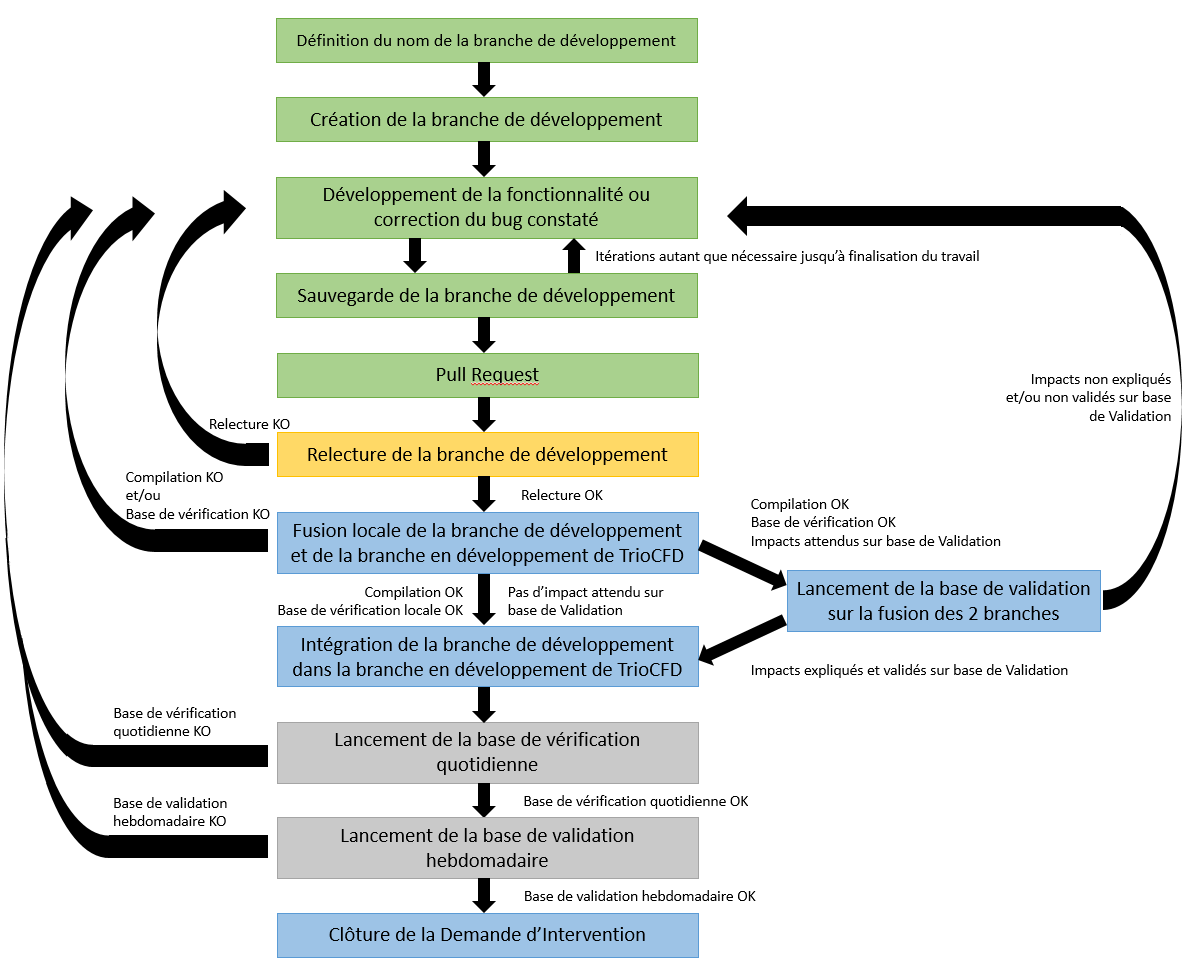
\includegraphics[width=16cm]{pictures/workflow_GIT.png}
   \vspace*{0.2cm}
   \captionof{figure}{\label{figure:workflow_GIT}Worflow de TrioCFD sous GIT pour une branche de développement - en vert : tâches développeur - en jaune : tâche relecteur - en bleu : tâche intégrateur - en gris : tâches Atelier Logiciel}
\end{figure}
\vspace{0.2cm}
En plus de garantir une bonne traçabilité pour tout changement apporté dans le code, cette méthodologie permet d'avoir une lecture facilitée de la base GIT du code. Quand cette méthodologie est étendue à tous les développements en cours sur le code, le flux sur GIT pour TrioCFD peut être illustré par la figure \ref{figure:workflow_GIT2}. L'ensemble de cette méthodologie est décrite sur le MediaWiki du projet TrioCFD sur Tuleap (\url{https://codev-tuleap.intra.cea.fr/plugins/mediawiki/wiki/triocfd/index.php?title=Accueil})\vspace{0.5cm}\\

La branche \texttt{triou/TMA} correspond donc à la version en développement de TrioCFD qui évolue au gré des intégrations en continu dans le code et sur laquelle tous les développeurs du code CEA doivent travailler. La branche \texttt{master}, quant à elle, est mise à jour à chaque sortie de version et correspond à la dernière version livrée du code. A la mise à jour de la branche \texttt{master} pour la sortie de version, un tag est également apposé et nommé suivant le numéro de la version livrée.\\
\begin{figure}[H]
   \centering
   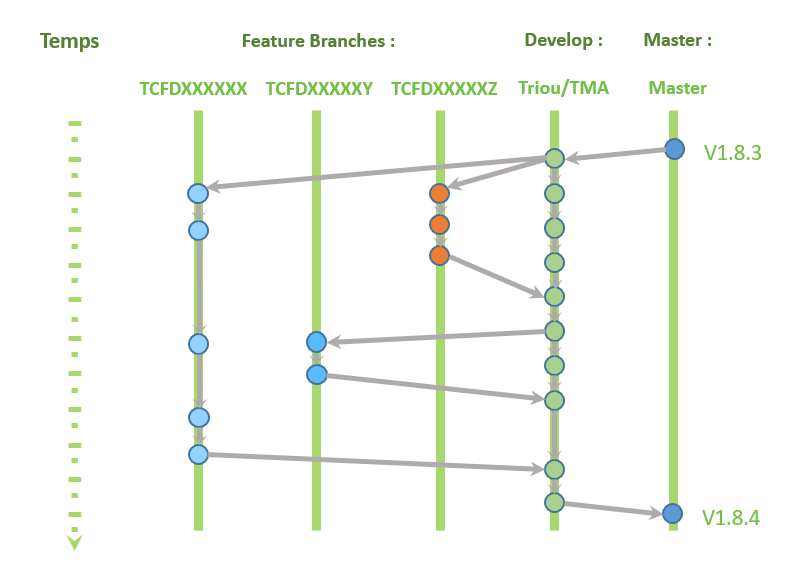
\includegraphics[width=16cm]{pictures/workflow_GIT2.png}
   \vspace*{0.2cm}
   \captionof{figure}{\label{figure:workflow_GIT2}Worflow général de TrioCFD sous GIT}
\end{figure}
\vspace{0.2cm}
La branche \texttt{triou/TMA} est mise à jour quotidiennement par l'Atelier de Génie Logiciel sur le dépôt extérieur de TrioCFD hébergé sur GITHUB à cette adresse : \url{https://github.com/cea-trust-platform/TrioCFD-code}. Ce dépôt extérieur permet aux développeurs hors CEA de travailler de la même façon que les développeurs CEA avec une version en développement du code à jour, nommée \texttt{next} sur GITHUB. Pour ce faire, ils créent également une \texttt{Issue} (qui est l'équivalent d'une Demande d'Intervention sur Tuleap) et nomment leur branche, en fonction, sous GITHUB. Afin de centraliser sur un seul Tracker l'ensemble des actions concernant TrioCFD, le Responsable de Code aura la charge de basculer l'ensemble des données présentes sur GITHUB sur Tuleap et renommer la branche de GITHUB en conséquence sur GIT avant son intégration dans le code.
\chapter{\label{chapitre:messagerie}Messagerie}
\lhead{Messagerie}
\rhead{OUTILS}

Afin d'échanger avec la TMA, une adresse de messagerie est \`a disposition des utilisateurs : \href{mailto:trust@cea.fr}{trust@cea.fr}. Cette adresse est exclusivement g\'er\'ee par la TMA.\\
Il s'agit de l'unique moyen de contact entre les utilisateurs du code et l'équipe de TMA. L'adresse personnelle des agents TMA n'est pas utilisée dans le cadre du projet. Cette boîte unique permet de conserver un historique complet des échanges de la TMA avec les utilisateurs. Chaque membre de l'équipe TMA a les droits en lecture et écriture sur cette messagerie.\\
Elle est utilisée pour répondre aux questionnements des utilisateurs mais également pour communiquer des informations pratiques pour les sessions de formations par exemple. Le délai contractuel de traitement des mails re\c cus via cette adresse par l'équipe TMA est d'un jour ouvré. Il est donc fortement recommandé de passer exclusivement par ce biais pour contacter le support (cela n'empêche cependant pas de mettre en copie le RPL ou le Responsable de Code) afin de garantir la bonne tra\c cabilité des échanges et d'être également assuré d'avoir un retour dans les plus brefs délais.


%\chapter{G\'en\'eration de la documentation}
%\lhead{G\'en\'eration de la documentation}
%\rhead{OUTILS}
%\newpage

\chapter{Interfa\c cage pour l'utilisateur et le d\'eveloppeur}
\lhead{Interfa\c cage pour l'utilisateur et le d\'eveloppeur}
\rhead{OUTILS}
Plusieurs scripts et outils sont à la disposition des utilisateurs afin de faciliter l'utilisation de la plateforme TRUST/TrioCFD. Une procédure est dédiée à chaque action effectuée sur la plateforme. Ces outils étant nombreux, ils n'ont pas pu tous être détaillés pour la première version de ce document mais cette partie sera étayée au fil des différentes versions.
\subsection{\label{subsec:install}Installation et compilation de TrioCFD}
On considère qu'une version TRUST au même niveau de développement est à disposition. On commence par charger l'environnement de TRUST de cette version :
\begin{lstlisting}
> source trust-code/env_TRUST.sh
\end{lstlisting}
On configure le passage en mode "Baltik" :
\begin{lstlisting}
> baltik_build_configure
\end{lstlisting}
On lance la configuration de TrioCFD :
\begin{lstlisting}
> ./configure
\end{lstlisting}
On lance la compilation de TrioCFD dans le mode souhaité:
\begin{lstlisting}
> make optim semi-optim debug
\end{lstlisting}

\subsection{Lancement d'un cas test}
Pour lancer un calcul en mode séquentiel, la méthodologie est la suivante :
\begin{lstlisting}
> cd $my_test_directory
> trust my_data_file %whitout .data
\end{lstlisting}
Il s'agit du lancement standard d'un calcul. D'autres options sont disponibles pour effectuer cette action et sont détaillés ci-après. La syntaxe de lancement devient alors :
\begin{lstlisting}
> trust [option] my_data file [nb_cpus] [1>file.out] [2>file.err]
\end{lstlisting}
où \texttt{nb\_cpus} correspond au nombre de processeurs utilisés pour lancer le calcul (ce nombre doit être égal au nombre de sous-domaines définis dans le jeu de données),\\
où les \texttt{options} disponibles sont :
\begin{table}[H]
\begin{centering}
%\scriptsize
\small
\begin{tabular}{Sl Sl}
\hline\hline
\rowcolor{lightgray}\textbf{OPTION} & \textbf{Description} \tabularnewline
\hline
-help | -h & List options \tabularnewline \hline
-baltik & Instanciate an empty Baltik project \tabularnewline \hline
-index & Access to the TRUST ressource index \tabularnewline \hline
-doc & Access to the TRUST manual (Generic Guide) \tabularnewline \hline
-config nedit|vim|emacs|gedit & Configure nedit or vim or emacs with TRUST keywords \tabularnewline \hline
-edit & Edit datafile \tabularnewline \hline
-xedit & Edit datafile with xdata \tabularnewline \hline
-xcheck & Check the datafile’s keywords with xdata \tabularnewline \hline
-partition & Partition the mesh to prepare a parallel calculation \tabularnewline
&(Creation of the .Zones files) \tabularnewline \hline
-mesh & Visualize the mesh(es) contained in the data file \tabularnewline \hline
-probes & Monitor the TRUST calculation only  \tabularnewline \hline
-evol & Monitor the TRUST calculation (new IHM) \tabularnewline \hline
-wiz & Create a TRUST datafile from a MED file (new IHM) \tabularnewline \hline
-prm & Write a prm file \tabularnewline \hline
-clean & Clean the current directory from all the generated
files by TRUST \tabularnewline \hline
-search keywords & Know the list of test cases from the data bases which contain keywords \tabularnewline \hline
-copy & Copy the test case datafile from the TRUST database
under the \tabularnewline
& present directory \tabularnewline \hline
-check all|testcase|list & Check the non regression of all the test cases or a single test case or a list \tabularnewline
& of tests cases specified in a file \tabularnewline \hline
-check function|class|class::method & Check the non regression of a list of tests cases covering a function, \tabularnewline
& a class or a class method\tabularnewline \hline
-gdb & Run under gdb debugger \tabularnewline \hline
-valgrind & Run under valgrind \tabularnewline \hline
-valgrind\_strict & Run under valgrind with no suppressions \tabularnewline \hline
-create\_sub\_file & Create a submission file only \tabularnewline \hline
-prod & Create a submission file and submit the job on the
main production class \tabularnewline 
& with exclusive resource \tabularnewline \hline
datafile -help\_trust & Print options of TRUST\_EXECUTABLE [CASE[.data]] [options] \tabularnewline \hline
\hline
\end{tabular}
\normalsize
\par\end{centering}
\caption{\label{tab:option-cas}Options disponibles pour le lancement d'un cas-test}
\end{table}
%%%%%%%%%%%%%%%%%%%%%%%%%%%%%%%%%%%%%%%%%%%%%%%%%%%%%%%%%%%%%%%%%%%%%%%%%%%%%%%%%%%%%%
%\part{\label{partie:outils}Bo\^ite \`a Outils}
%\normalsize \normalfont
%\input{./part4-boite.tex}
%%%%%%%%%%%%%%%%%%%%%%%%%%%%%%%%%%%%%%%%%%%%%%%%%%%%%%%%%%%%%%%%%%%%%%%%%%%%%%%%%%%%%%
\part{\label{partie:v&v}Description des Outils de V\'erification et Validation}
\normalsize \normalfont
\rhead{DESCRIPTION DES OUTILS DE V\&V}

\lettrine[lines=2,slope=0pt,nindent=4pt]{\textbf{P}}{our} tout code, les processus de V\'erification et Validation sont primordiaux puisqu'ils permettent de conna\^itre l'\'etat du code \`a tout moment et de garantir son comportement sur un large panel de cas allant des plus simples aux plus compliqu\'es. Ces 2 processus ont des objectifs diff\'erents : Le processus de \textbf{V\'erification} permet de s'assurer que les \'equations sont \textbf{correctement} r\'esolues tandis que le processus de \textbf{Validation} permet de v\'erifier que \textbf{les} bonnes \'equations sont r\'esolues.\newline
Dans cette partie, l'application de ces 2 processus dans le code \texttt{TrioCFD} sera d\'etaill\'ee.\smallskip\newline
Une autre notion est \'egalement extrêmement importante dans le processus de V\&V du code, \`a savoir la portabilit\'e du code. En effet, un code de calcul doit \^etre le moins sensible possible \`a l'environnement sur lequel il est utilis\'e que ce soit la configuration mat\'erielle (processeur) ou l'environnement logiciel (syst\`eme d'exploitation, compilateur,...). Ainsi, afin d'avoir la meilleure portabilit\'e possible, un code ne doit utiliser que la biblioth\`eque logicielle "standard" disponible sur plusieurs environnements et non pas certaines fonctions sp\'ecifiques \`a un environnement particulier. Le code pourra ainsi \^etre port\'e sans difficult\'e d'une machine à l'autre en le recompilant avant utilisation. Gr\^ace \`a l'utilisation de biblioth\`eques "standard", le code est alors adapt\'e \`a un plus grand nombre d'utilisateurs.\newline

Afin de garantir une bonne portabilit\'e de la plateforme \texttt{TRUST/TrioCFD}, des biblioth\`eques n\'ecessaires, plus riches que les biblioth\`eques communes sont fournies, pour chaque version, dans les \texttt{externalpackages} de TRUST (\textit{e.g.} PETSc, Miniconda,...). La plateforme \texttt{TRUST/TrioCFD} dispose donc d'une bonne portabilit\'e native. La surveillance r\'eguli\`ere de celle-ci permet donc de s'assurer qu'aucun codage ambigu ou non conforme soit introduit par inadvertance dans le code. Celui-ci pourrait \^etre interprété diff\'eremment suivant l'environnement consid\'er\'e, entra\^inant des \'ecarts inexpliqu\'es. Le diagnostic de ce genre de probl\`eme \'etant souvent complexe \`a \'etablir, une identification au plus t\^ot permet alors de rectifier rapidement. Pour ce faire, \texttt{TRUST} et \texttt{TrioCFD} sont test\'es quotidiennement sur un large panel de configurations qui sera cartographi\'e dans le premier chapitre de cette partie.

%%%%%%%%%%%%%%%%%%%%%%%%%%%%%%%%%%%%%%%%%%%%%%%%%%%%%%%%%%%%%%%%%%%%%%%%%%%%%%%%%%%%%%%%%%%%%%%%%%%%%%%%%%%%%%%%%%%%%

\chapter{\label{parc}Parc des machines}
\lhead{Parc des machines}
\rhead{DESCRIPTION DES OUTILS DE V\&V}

Afin de s'assurer de la bonne portabilit\'e de \texttt{TrioCFD}, un parc d'un peu plus de vingt de machines, pr\'esentant des configurations distinctes, a \'et\'e mis en place et est r\'eguli\`erement mis \`a jour au en fonction de l'\'evolution des syst\`emes d'exploitation, compilateurs et autres biblioth\`eques. En voici la constitution : \smallskip\newpage

\begin{table}[H]
\begin{centering}
%\scriptsize
\tiny
\begin{tabular}{Sc Sc Sc Sc Sc Sc Sc Sc}
\hline\hline
\rowcolor{lightgray}\textbf{CIBLE} & \textbf{CORES} & \textbf{RAM} & \textbf{CACHE} & \textbf{FREQ.} & \textbf{OS} & \textbf{COMPILATEUR} & \textbf{MPI} \tabularnewline
\hline
cluster1-amd-gpu & 8 & 131 & 512 & 2095 & CentOS release 7.6.1810 & g++ 9.1.0 & OpenMPI 3.1.4 \tabularnewline \hline %orcus
cluster1-amd & 8 & 131 & 512 & 2095 & CentOS release 7.6.1810 & icpc 19.0.3.199 & Intel MPI 2019 \tabularnewline \hline %orcus
cluster1-intel & 8 & 97 & 16896 & 2300 & CentOS release 7.6.1810 & icpc 19.0.3.199 & Intel MPI 2019 \tabularnewline \hline %orcus
cluster2 & 56 & 131 & 19712 & 3157 & CentOS release 7.9.2009 & g++ 4.8.5 & MPICH 3.2 \tabularnewline \hline %pegasi2
cluster3 & 8 & 131 & 35840 & 2401 & Red Hat Server release 7.9 & icpc 18.0.3 & OpenMPI 4.0.2rc3 \tabularnewline \hline %cobalt
cluster4-amd-build64 & 8 & 263 & 512 & 2500 & Red Hat Server release 7.9 & icpc 19.1.3.304 & OpenMPI 4.0.2rc3 \tabularnewline \hline %irene
cluster4-amd-gpu & 8 & 263 & 512 & 2500 & Red Hat Server release 7.9 & g++ 8.3.0 & OpenMPI 4.0.2rc3 \tabularnewline \hline %irene
cluster4-amd & 8 & 263 & 512 & 2500 & Red Hat Server release 7.9 & icpc 19.1.3.304 & OpenMPI 4.0.2rc3 \tabularnewline \hline %irene
cluster4-build64 & 8 & 196 & 33792 & 2701 & Red Hat Server release 7.9 & icpc 19.0.5.281 & OpenMPI 4.0.2rc3 \tabularnewline \hline %irene
cluster4 & 8 & 263 & 512 & 2500 & Red Hat Server release 7.9 & icpc 19.1.3.304 & OpenMPI 4.0.2rc3 \tabularnewline \hline %irene
station1 & 6 & 16 & 9216 & 3989 & CentOS release 7.9.2009 & g++ 4.8.5 & MPICH 3.2 \tabularnewline \hline %is154711
station2 & 8 & 8 & 8192 & 1596 & CentOS release 7.9.2009 & g++ 4.8.5 & MPICH 3.2 \tabularnewline \hline %is210968
station3 & 24 & 16 & 12288 & 2538 & Ubuntu 18.04.5 LTS & g++ 7.5.0 & MPICH 3.2 \tabularnewline \hline %is212912
station4 & 4 & 8 & 6144 & 3199 & Ubuntu 16.04.7 LTS & g++ 5.4.0 & MPICH 3.2 \tabularnewline \hline %is212957
station5 & 24 & 16 & 12288 & 1596 & CentOS release 7.9.2009 & g++ 4.8.5 & MPICH 3.2 \tabularnewline \hline %is212958
station6 & 12 & 12 & 12288 & 1801 & Ubuntu 20.04.2 LTS & g++ 9.3.0 & MPICH 3.2 \tabularnewline \hline %is213122
station7 & 4 & 8 & 8192 & 3402 & Fedora release 24 & g++ 6.1.1 & MPICH 3.2 \tabularnewline \hline %is221710
station8 & 24 & 32 & 15360 & 1200 & CentOS release 6.4 & g++ 10.3.0 & MPICH 3.2 \tabularnewline \hline %is223196
station9 & 24 & 32 & 15360 & 1340 & Fedora release 26 & g++ 7.1.1 & MPICH 3.2 \tabularnewline \hline %is223288
station10 & 4 & 16 & 8192 & 3311 & CentOS release 7.9.2009 & g++ 4.8.5 & MPICH 3.2 \tabularnewline \hline %is230500
station11 & 4 & 16 & 8192 & 1501 & CentOS release 7.9.2009 & g++ 4.8.5 & MPICH 3.2 \tabularnewline \hline %is231771
station12 & 4 & 16 & 8192 & 3157 & CentOS release 7.9.2009 & g++ 4.8.5 & OpenMPI 2.0.4 \tabularnewline \hline %is232974
station13 & 32 & 65 & 11264 & 800 & Ubuntu 18.04.5 LTS & g++ 7.5.0 & MPICH 3.2 \tabularnewline \hline %is234617
station14 & 6 & 16 & 9216 & 3910 & CentOS release 7.9.2009 & g++ 4.8.5 & MPICH 3.2 \tabularnewline \hline %is241478
station15 & 6 & 16 & 9216 & 3964 & CentOS release 7.9.2009 & g++ 4.8.5 & MPICH 3.2 \tabularnewline \hline %is241479
station16 & 16 & 16 & 16384 & 2551 & Fedora release 30 & g++ 9.0.1 & MPICH 3.2 \tabularnewline \hline %is241762
station17 & 12 & 32 & 8448 & 1673 & Ubuntu 20.04.2 LTS & g++ 9.3.0 & MPICH 3.2 \tabularnewline \hline %is242979
station18-clang & 8 & 32 & 12288 & 3600 & Fedora release 32 & clang++ 10.0.0 & OpenMPI 2.0.4 \tabularnewline \hline %is242981
station19-gpu & 8 & 32 & 12288 & 4514 & Fedora release 32 & cuda-g++ 8.3.0 & OpenMPI 4.1.0 \tabularnewline \hline %is242981
cluster5-build64 & 8 & 263 & 512 & 2184 & Red Hat release 8.3 & icpc 19.1.3.304 & OpenMPI 4.0.5 \tabularnewline
\hline\hline
\end{tabular}
\normalsize
\par\end{centering}
\caption{\label{tab:Computer-characteristics}Parc des machines de tests de \texttt{TrioCFD}}
\end{table}
C'est sur ce parc de machines que sont lanc\'ees la v\'erification et la validation.
\newpage

%%%%%%%%%%%%%%%%%%%%%%%%%%%%%%%%%%%%%%%%%%%%%%%%%%%%%%%%%%%%%%%%%%%%%%%%%%%%%%%%%%%%%%%%%%%%%%%%%%%%%%%%%%%%%%%%%%%%%

\chapter{\label{chapitre:verification}Base de V\'erification}
\lhead{Base de V\'erification}
\rhead{DESCRIPTION DES OUTILS DE V\&V}

\subsection{Objectifs et \'etapes de la V\'erification}

Le processus de \textbf{V\'erification} a pour but de s'assurer que le code satisfait pleinement toutes les exigences attendues. La v\'erification doit r\'epondre \`a la question suivante : " Est-ce que nous construisons le code correctement ? " Cela correspond \`a v\'erifier que les sp\'ecifications sont correctement mises en \oe uvre par le syst\`eme. Elle permet de d\'eterminer si le r\'esultat d'une phase de d\'eveloppement donn\'ee satisfait les conditions impos\'ees au d\'ebut de cette phase. La v\'erification du logiciel garantit que celui-ci a \'et\'e bien construit et confirme que le code r\'epond aux plans des d\'eveloppeurs.\smallskip\newline


La v\'erification quotidienne porte sur les aspects suivants :\newline
\begin{itemize}[label=$\Rightarrow$, font=\LARGE]
  \item \textbf{la bonne compilation du code :} toutes les nuits, la compilation du code est lanc\'ee en mode optimis\'e et semi-optimis\'e sur plusieurs machines du parc sur la branche de d\'eveloppement (branche triou/TMA). La compilation en mode debug est lanc\'ee tous les week-end car ce mode de compilation n\'ecessite un temps trop cons\'equent au vu des contraintes du temps d'occupation des machines du parc. En cas de non succ\'es de la compilation, la version de d\'eveloppement du code est consid\'er\'ee comme \'etant en d\'efaut et un correctif doit lui \^etre approt\'ee dans les plus brefs d\'elais.
  \item \textbf{la bonne r\'ealisation des cas-tests :} apr\`es la compilation, la base de cas-tests (comprenant \`a la fois des tests \'el\'ementaires et des tests issus des fiches de validation) est lanc\'ee sur 3 pas de temps. On s'attache \`a v\'erifier que ces 3 pas de temps ont \'et\'e r\'ealis\'es avec succ\`es mais \'egalement que les r\'esultats physiques obtenus sur ces 3 pas de temps sont conformes aux r\'esultats attendus. Pour ce faire, les r\'esultats   attendus sur ces 3 pas de temps sont stock\'es en gestion de configuration dans la base GIT du code sous la forme de fichiers lml zipp\'es (fichiers .lml.gz). Les r\'esultats obtenus avec la v\'erification sont alors compar\'es sous format binaire avec les r\'esultats en gestion de configuration (attendus). En cas d'interruption de cas-tests ou de non-conformit\'e des r\'esultats physiques avec l'attendu, le code est consid\'er\'e comme d\'efaillant. Une action doit \^etre men\'ee, soit sur le code, soit sur le(s) cas-test afin de r\'etablir la situation. 
  \item \textbf{la portabilit\'e du code :} la compilation du code ainsi que la base de tests de v\'erification sont lanc\'ees sur des ordinateurs ou stations de travail ayant diff\'erentes configurations mat\'erielles et/ou logicielles (voir chapitre \ref{parc}). Sur chacune de ces machines, la version de d\'eveloppement du jour de TrioCFD doit remplir correctement les deux crit\`eres pr\'ec\'edents (compilation et r\'ealisation de la base de cas-test), assurant la bonne portabilit\'e quotidienne du code.
  \item \textbf{la g\'en\'eration de la documentation :} la bonne g\'en\'eration de la documentation est \'egalement test\'ee toute les nuits. Toutefois, \`a l'heure actuelle, l'ensemble de la documentation n'est pas test\'e. Seul le TrioCFD Reference Manuel, construit \`a partir de balises XDATA pr\'esentes dans le code (voir paragraphe), l'est. La g\'en\'eration automatique de l'ensemble de la documentation et sa vérification constituent une voie d'am\'elioration d'ores et déjà identifiée.
\end{itemize}\smallskip

\subsection{La base de cas-tests de \texttt{TrioCFD}}

Revenons maintenant un peu plus en d\'etails sur la base de cas-tests de \texttt{TrioCFD}. Celle-ci comprend 1533 tests s\'equentiels et 444 tests parall\`eles (voir tableau r\'ecapitulatif en Annexe). Ces cas-tests couvrent l'ensemble des baltiks de \texttt{TrioCFD} et assurent un taux de couverture de 80.05\% des mot-cl\'es (1349 mots-cl\'es sont test\'es sur les 1685 mots-cl\'es de \texttt{TrioCFD}). Les cas-tests sont rang\'es dans le repertoire \texttt{tests} de chacun des baltiks. Un cas-test a pour extension \texttt{.data} et peut \^etre soit un test simple (test de R\'ef\'erence), soit un test extrait d'une fiche de validation. Dans ce dernier cas, comme une fiche de validation peut comporter plusieurs cas-tests, il aura un suffixe de la forme \texttt{\_jddX.data} o\`u X variera de 1 au nombre de jeux de donn\'ees de la fiche de validation.\newline
Chaque cas-test \texttt{.data} est rang\'e dans un r\'epertoire du m\^eme nom qui contient \'egalement le r\'esultat de r\'ef\'erence de ce cas-test (fichier au format \texttt{.lml.gz}). Comme mentionn\'e pr\'ec\'edemment, ces cas-tests sont lanc\'es sur les 3 premiers pas de temps dans le cadre du processus de v\'erification afin de s'assurer que :
\begin{itemize}[label=$\Rightarrow$, font=\LARGE]
  \item le calcul se d\'eroule correctement sur ces 3 pas de temps ;
  \item les r\'esultats obtenus sur ces 3 pas de temps ne pr\'esentent pas d'\'ecarts avec les r\'esultats de   r\'ef\'erence.
\end{itemize}
Afin que la base de v\'erification puisse \^etre lanc\'ee aussi souvent que n\'ecessaire, son temps de r\'ealisation doit rester abordable. Sur un poste de travail standard (\textit{e.g.} is241762 - voir tableau \ref{tab:Computer-characteristics}), les 1977 cas-tests s'exécutent en 2047.2s (2s/test), soit un peu moins d'une heure, le plus long test durant 89 secondes.


\subsection{Fréquence de lancement de la base de cas-tests de \texttt{TrioCFD}}

Chaque nuit, l'Atelier de G\'enie Logiciel lance, sur les diff\'erentes machines du parc, la v\'erification de \texttt{TrioCFD}. Ces machines, correspondant, pour la plupart aux stations de travail des d\'eveloppeurs, ne peuvent donc \^etre utilis\'ees pour la v\'erification en dehors des heures de travail. Par cons\'equent, le processus de v\'erification quotidien doit \^etre men\'e sur un temps d'ex\'ecution raisonnable durant la semaine. La v\'erification plus pouss\'ee aura lieu durant le week-end. La base de vérification est automatiquement lanc\'ee tous les soirs \`a 19h15 et est stopp\'ee \`a 7h le matin si elle n'est pas parvenue \`a terme.\smallskip\newline

Outre son lancement quotidien automatique, le d\'eveloppeur doit s'assurer de son bon fonctionnement avant chaque demande d'int\'egration (Pull-Request) dans le code, v\'erification qui devra \^etre de nouveau effectu\'ee par l'int\'egrateur avant d'int\'egrer une branche de d\'eveloppement/correction dans la branche de d\'eveloppement de TrioCFD (branche \texttt{triou/TMA}) (voir chapitre \ref{chapitre:GIT}).

\subsection{Méthodologie de lancement de la base de cas-tests de \texttt{TrioCFD}}
Pour le lancement de la base de vérification de façon manuelle, l'utilisateur doit avoir préalablement compilé sa branche de développement de TrioCFD (suivant la procédure détaillée dans la section \ref{subsec:install}). Il crée alors le lien vers la version compilée et peut lancer la base de vérification de la façon suivante :
\footnotesize
\begin{lstlisting}
> source env_TrioCFD.sh    % source de l'environnement de TrioCFD
> make check_all_optim     % lancement de la base de verification
\end{lstlisting}
\normalsize

Une fois la base de vérification terminée, la procédure renvoie le bilan de celle-ci , dont un exemple peut être visualisé sur la figure \ref{figure:verif-resultats}.\medskip\newline

\begin{figure}[H]
   \centering
   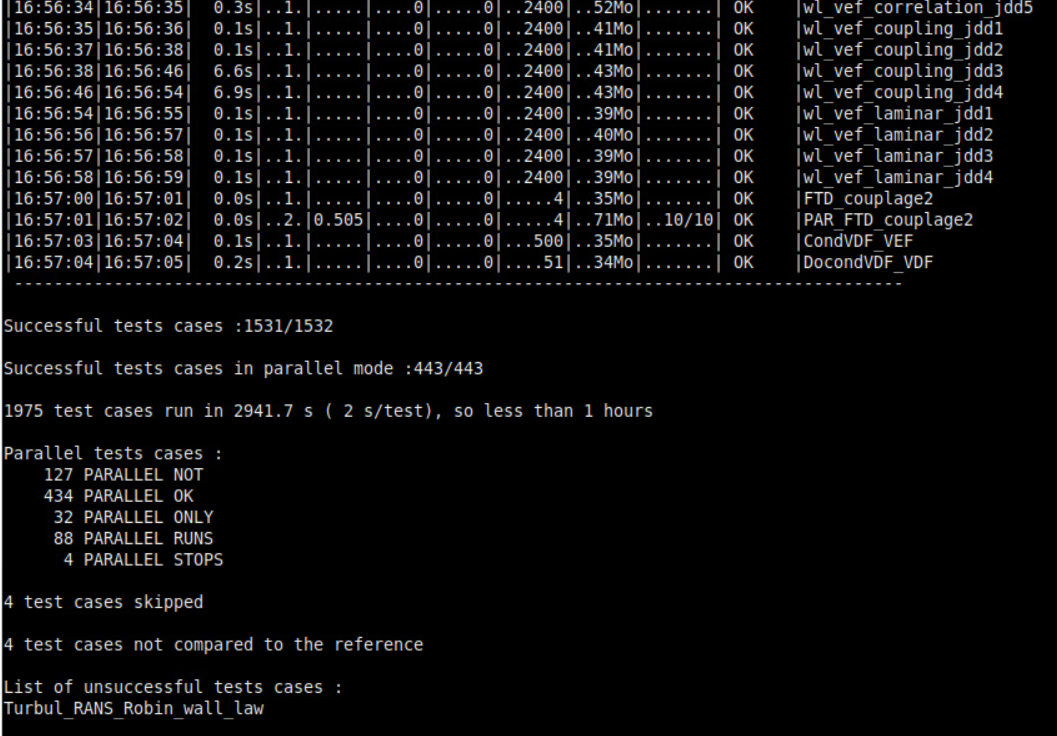
\includegraphics[width=16cm]{pictures/verif-resultats.png}
   \vspace*{0.2cm}
   \captionof{figure}{\label{figure:verif-resultats}Exemple de bilan du lancement de la base de vérification lancée en local}
\end{figure}


Pour le lancement automatique quotidien, l'atelier de TrioCFD, contenant un ensemble de procédures en Bash et en Python, est exécuté chaque soir par l'atelier de TRUST par un crontab (procédure de lancement automatique et périodique) sur le script \texttt{lance\_test\_nuit} contenu dans le répertoire \texttt{bin/admin} de TRUST. Ce script met à jour TrioCFD par rapport à ce qui a été intégré la veille dans la branche \texttt{triou/TMA}, installe TRUST, puis envoi TriocCFD (et les autres baltiks sur base TRUST) sur les machines du parc (voir tableau \ref{tab:Computer-characteristics}).
Les machines sur lesquelles TRUST et ses Baltiks sont testés chaque nuit sont spécifiées dans le fichier \texttt{bin/admin/liste.machines} de TRUST. Les machines concernant TrioCFD sont celles qui contiennent le paramètre -TrioCFD dans ce fichier au niveau de la colonne \texttt{baltiks}. Ce fichier contient également les options de compilation et de lancement des tests. Quelques-unes de ces options sont données dans le tableau \ref{tab:options-verif}.

\begin{table}[H]
\begin{centering}
\footnotesize
\begin{tabular}{Sc Sc}
\hline\hline
\rowcolor{lightgray}\textbf{Option} & \textbf{Signification}  \tabularnewline
\hline
-g & lancement des cas tests en mode debug \tabularnewline \hline
-semi\_opt & lancement des cas tests en mode semi optimisé \tabularnewline \hline
-gui & test des balises XDATA (génération Référence Manual) \tabularnewline \hline
-clang & permet de spécifier un compilateur CLANG (variante de compilateur - par défaut GNU) \tabularnewline \hline
-cuda & lancement des tests sur les GPC - par défaut sur les CPU \tabularnewline \hline
-gcov & test la couverture des mots clés par la base de vérification \tabularnewline \hline
-limited & lance une base plus succincte de cas tests (20)\tabularnewline \hline 
-all & lance l'ensemble des cas tests)\tabularnewline \hline
-build\_64\_bit & lancement sur 64 bits \tabularnewline \hline 
-test & lancement des cas tests de TRUST avec l'exécutable de TrioCFD \tabularnewline \hline
-platform & profiling : analyse les temps de passage dans les différentes parties du code \tabularnewline \hline
-disable-mpi & désactive le lancement en parallèle des cas tests \tabularnewline \hline
-download-visit & télécharge la dernière version de Visit plutôt que d'utiliser la version présente dans TRUST  \tabularnewline 
\hline\hline
\end{tabular}
\normalsize
\par\end{centering}
\caption{\label{tab:options-verif}Liste des options utilisées par l'atelier logiciel pour le lancement de la base de vérification}
\end{table}

Le script \texttt{lance\_test\_nuit} installe d'abord TrioCFD sur la machine de l'atelier, puis crée un fichier qui permet de spécifier les options de compilation et de tests pour chacune des machines distantes. Ce fichier s'appelle Run.liste et contient autant de lignes de machines et spécifie, entre autre, le nom de la machine, le chemin vers TRUST, le chemin d'installation, le mode de tests,..\\
Le lancement des installations sur les machines distantes se fait avec le script \texttt{/export/home/\-triou/tuleap/Livraison/TRUST/bin/baltik/share/baltik/bin/baltik\_check\_portability Run.liste}. Ce script va :
\begin{enumerate}
\item créer l'archive triocfd.tar, qui contient le triocfd.tar.gz et les autres scripts pour préparer, installer, configurer, vérifier, ..
\item la copier sur chacune des machines distantes et lancer la compilation
\item récupérer les logs en local de chacune des machines et générer la page nuit\_triocfd.html qui permettra l'analyse des résultats de vérification.
\end{enumerate}


Le script \texttt{lance\_test\_nuit} rapatrie les résultats de TRUST à 7h du matin, et stoppe la procédure de vérification de TrioCFD sur les machines pour lesquelles l'installation ou les tests ne sont pas terminés. Ceci garantit que la page nuit\_triocfd.html est correctement générée. Cette page servira au dépouillement des résultats de la base de vérification.


\subsection{Dépouillement des résultats de la base de cas-tests de \texttt{TrioCFD}}

L'analyse des résultats obtenus par la base de vérification de TrioCFD commence par l'analyse de la page html générée par le script \texttt{lance\_test\_nuit} (voir figure \ref{figure:trio_verif}). Cette page de rapport a été refondue en 2021 afin de faire figurer les éléments nécessaires pour analyser efficacement les résultats de la base de vérification.\smallskip\\
 Elle est composée de 15 colonnes, les colonnes 1, 4, 5 et 6 donnent les informations générales sur les machines testées (nom, OS, architecture, et compilateur C++). Les colonnes 2 et 3 renseignent sur la date et l'heure de démarrage de l'atelier de vérification sur chacune des machines. La $7^{ème}$ colonne identifie si la machine est considérée comme une machine cible (machine sur laquelle le succès de la vérification est indispensable pour considérer la version du jour comme stable). Ces machines sont au nombre de 4 sur TrioCFD. Elles correspondent à des machines présentant une configuration standard en terme d'OS et compilateur par rapport aux machines des utilisateurs/développeurs. Ainsi, si l'atelier de vérification ne fonctionne pas sur ces machines cibles, l'utilisation du code sera dégradée dans l'équipe. La $13^{ème}$ colonne correspond au mode de compilation de de TrioCFD sur la machine concernée. Toutes les autres colonnes sont quant à elles destinées à l'analyse de la base de vérification :\\
\begin{itemize}[label=$\Rightarrow$, font=\LARGE]
   \item \textbf{Colonne 8 - prepare} : vérifie que le désarchivage de l'archive envoyée par la machine de l'atelier s'est bien déroulé et génère les scripts de lancement propres à chaque machine (configure.sh, make.sh,...) en fonction des options définies dans le fichier \texttt{liste.machines}
   \item \textbf{Colonne 9 - configure} : vérifie que la configuration de TrioCFD s'est bien déroulée (commandes \texttt{baltik\_build\_configure et \texttt{./configure}}
   \item \textbf{Colonne 10 - make} : vérifie que la compilation de TrioCFD a été faite avec succès en respectant les options de compilations spécifiées
   \item \textbf{Colonne 11 - make\_check} : lancement des tests de vérification en respectant les options spécifiées dans le fichier \texttt{liste.machines}
   \item \textbf{Colonne 12 - make\_install} : vérifie que l'installation générale a été bien faite et le baltik bien chargé. Cet état est toujours valide si les 4 présents ont abouti avec succès. Cette colonne pourra être supprimée lors de la prochaine évolution de l'atelier de vérification
   \item \textbf{Colonne 14 - test\_par} : nombre de tests en mode parallèle réussis par rapport au nombre de tests lancés
   \item \textbf{Colonne 15 - test\_seq} : nombre de tests en mode séquentiel réussis par rapport au nombre de tests lancés
\end{itemize}

Le résultat pour chacune de ces 6 colonnes est analysable dans le détail en cliquant sur le lien présent dans chacune des cases qui renvoie aux fichiers \texttt{.log} ou \texttt{.err}. L'équipe TMA assure le suivi quotidien du bon déroulement de l'atelier de vérification. En cas de problème, l'équipe TMA et les Responsable de Code s'attacheront à résoudre au plus vite les problèmes constatés et aucune nouvelle intégration ne sera faite dans la branche en développement de TrioCFD tant que l'état de l'atelier de vérification ne sera pas revenu dans son état nominal. 
\newpage

\begin{figure}[H]
   \centering
   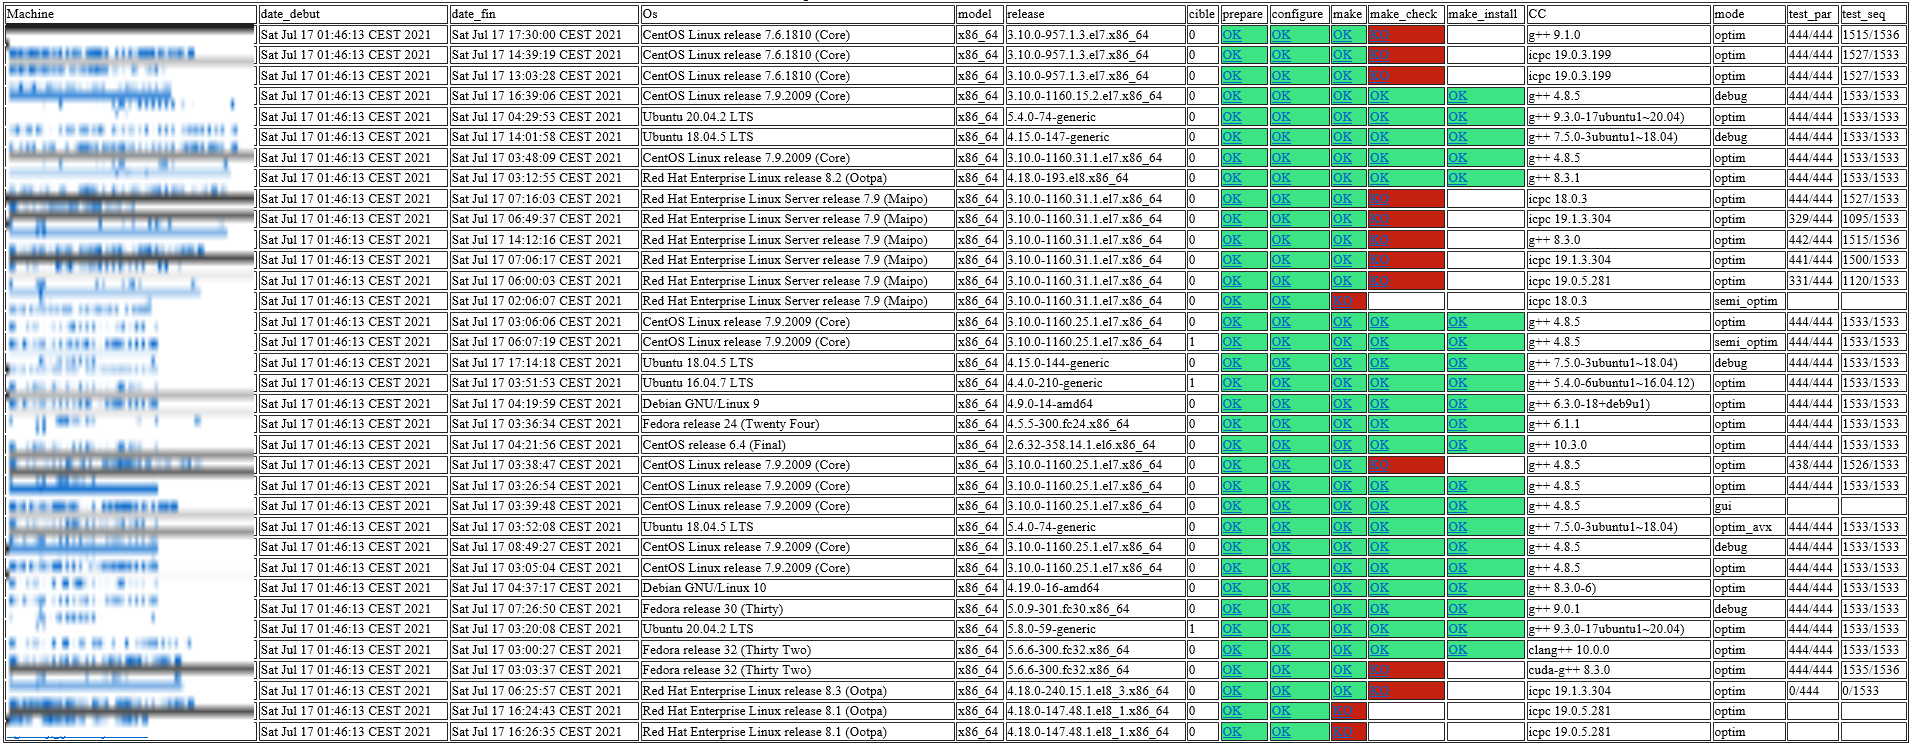
\includegraphics[width=23cm ,angle =90]{pictures/trio_verif_flou.png}
   \vspace*{0.2cm}
   \captionof{figure}{\label{figure:trio_verif}Page html générée pour l'analyse quotidienne de la base de vérification de TrioCFD}
\end{figure}




%%%%%%%%%%%%%%%%%%%%%%%%%%%%%%%%%%%%%%%%%%%%%%%%%%%%%%%%%%%%%%%%%%%%%%%%%%%%%%%%%%%%%%%%%%%%%%%%%%%%%%%%%%%%%%%%%%%%%

\chapter{\label{chapitre:validation}Base de Validation de TrioCFD}
\lhead{Base de Validation}
\rhead{DESCRIPTION DES OUTILS DE V\&V}
Si la v\'erification logicielle garantit que le r\'esultat de chaque phase du processus de d\'eveloppement logiciel r\'ealise effectivement les sp\'ecifications initiales (\textit{e.g.} impl\'ementation correcte des \'equations et mod\`eles sp\'ecifi\'es initialement), la validation logicielle garantit, quant \`a elle, que le produit logiciel r\'epond aux besoins de toutes les parties prenantes (\textit{e.g.} la bonne r\'esolution des \'equations d\'efinies dans les sp\'ecifications et r\'esultats physiques conformes \`a l'attendu).

\subsection{La base de validation de \texttt{TrioCFD}}

La  validation du code est effectuée via les fiches de validation (PRM). Ces PRM peuvent être composées d'un ou plusieurs cas tests de la base de vérification. Lorsqu'une fiche de validation est composée de plusieurs cas tests, c'est parce que ceux-ci comportent des variantes (différents maillages, différents modèles,...) La base de validation est actuellement composée de 162 fiches. Ce nombre est en perpétuelle augmentation puisqu'à chaque nouveau développement, le développeur se doit de fournir une fiche de validation associée.\\
Ces fiches de validation sont disponibles dans le répertoire \texttt{/share/Validation/Rapports\_automatiques} de chacun des Baltiks et peuvent être ensuite ordonnées dans différents sous-répertoires pour mieux identifier les sujets d'intérêt de chacune. A l'heure actuelle, cette sous-structuration n'est pas optimale et sera améliorée dans les futures versions de TrioCFD.\\
Le tableau récapitulatif des différentes fiches de validation est donné en Annexe A du document intitulé models\_report\_TrioCFD.pdf présent dans le répertoire \texttt{share/doc} de TrioCFD. Il sera amené à être prochainement migré vers le document validation\_report\_TrioCFD.pdf situé dans ce même répertoire.\\
La validation est actuellement exécutée sur une seule machine (cluster2 du tableau \ref{tab:Computer-characteristics}). Actuellement, seule cette machine est en mesure de faire tourner la base de validation : les autres clusters sont des machines partagées avec d'autres codes, le processus de validation nécessite trop de temps de calcul et les stations ne sont pas suffisamment puissantes pour que le processus de validation soit achevé dans des temps raisonnables. Prochainement, un nouveau cluster sera disponible pour la validation avec des caractéristiques de configuration différentes afin d'analyser la portabilité sur ce processus. Le processus de validation présente également une contrainte forte en terme de temps de résolution et doit être en mesure de fournir les résultats dans un délai acceptable. Avant la mise en service du cluster2, mi 2020, celui-ci était lancé sur une station de travail et prenait entre 12 et 13. Cette durée ne permettait pas de garantir une validation suffisamment performante du code.\\
La base de validation est exécutée sur le cluster via le code Open Source Jenkins, développé en Java, qui permet de bien gérer tous les processus d'un code en intégration continue comme TrioCFD. Jenkins est relativement ergonomique avec une interface graphique simple pour la création de files de tâches mais dispose également d'un mode un peu plus évolué avec la possibilité pour l'utilisateur d'implémenter ses propres scripts en langage Groovy. TrioCFD utilise ces deux fonctionnalités de Jenkins pour le lancement de la base de validation de TrioCFD.\\
La validation hebdomadaire du logiciel porte actuellement sur les aspects suivants :
\begin{itemize}[label=$\Rightarrow$, font=\LARGE]
   \item \textbf{la bonne compilation du code}
   \item \textbf{la bonne résolution des fiches de validation}
   \item \textbf{la bonne génération des fiches de validation}
\end{itemize}

Ce processus de validation sera prochainement enrichi afin d'être également en mesure de contrôler la portabilité du code de façon plus poussée que la base de vérification mais s'assure également de la bonne génération de la documentation utilisateur de TrioCFD.\\

\subsection{Fréquence de lancement de la base de validation de \texttt{TrioCFD}}
Avec l'arrivée du cluster2, la fréquence de lancement de la base de validation a pu être considérablement augmentée. En effet, elle tournait auparavant seulement avant chaque sortie de version à cause de sa durée trop conséquente. La réduction de cette durée permet maintenant de l'exécuter de façon hebdomadaire. Son lancement est actuellement réalisé manuellement par le Responsable de Code le vendredi, après que les dernières intégrations prévues dans la branche \texttt{triou/TMA} aient été réalisées. Ce lancement hebdomadaire est réalisé sur la branche en développement de TrioCFD en s'appuyant sur la version de même niveau de TRUST. Il sera prochainement automatisé.\\
Lorsque des développements pour lesquels des impacts sont prévus doivent être intégrés dans la version, la base de validation peut être amenée à être lancée à tout moment par le Responsable de Code.

\subsection{Méthodologie de lancement de la base de validation de \texttt{TrioCFD}}

La machine maître de lancement des tâches de Jenkins (Pipelines) est actuellement la station 9 du tableau \ref{tab:Computer-characteristics}. Un Pipeline spécifique a été créé pour le lancement de la validation, nommé TrioCFD\_Validation et rattaché au cluster 2. Ce Pipeline est lancé manuellement en remplissant la fiche de paramètres de la figure \ref{figure:lancement_jenkins}.

\begin{figure}[H]
   \centering
   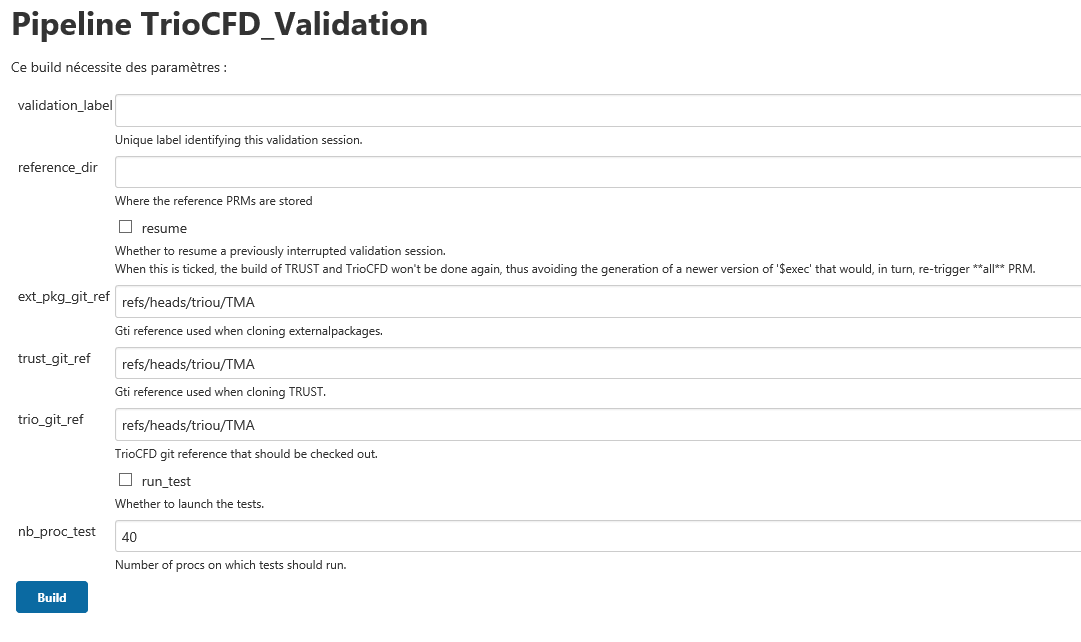
\includegraphics[width=16cm]{pictures/lancement_jenkins.png}
   \vspace*{0.2cm}
   \captionof{figure}{\label{figure:lancement_jenkins}Méthodologie de lancement du Pipeline de Validation de TrioCFD sous Jenkins}
\end{figure}
Six principaux paramètres sont à renseigner manuellement pour le lancement de la base de validation qui sont :
\begin{itemize}[label=$\Rightarrow$, font=\LARGE]
   \item \textbf{validation\_label} : nom du répertoire de validation résultant de ce lancement
   \item \textbf{reference\_dir} : nom du répertoire d'une version antérieure de validation par rapport à laquelle la version lancée sera comparée
   \item \textbf{ext\_pkg\_git\_ref} : branche, SHA1 ID ou tag du dépôt git de externalpackages à partir duquel la validation sera lancée
   \item \textbf{trust\_git\_ref} : branche, SHA1 ID ou tag du dépôt git de TRUST à partir duquel la validation sera lancée
   \item \textbf{trio\_git\_ref} : branche, SHA1 ID ou tag du dépôt git de TrioCFD à partir duquel la validation sera lancée
   \item \textbf{nb\_proc\_test} : nombre de processeurs de la machine sur laquelle le processus de validation sera lancé (par défaut 40)
\end{itemize}
Deux cases à cocher sont utilisées pour la réitération du lancement en cas de problème lors du précédent. La première, nommée \texttt{resume} permet de relancer le processus de validation à partir de l'endroit exact où celle-ci a été interrompu. La seconde, nommée \texttt{run\_test}, permet de s'affranchir de toute la première partie qui concerne le clonage des différentes bases git de la compilation de TRUST et TrioCFD.

Ce Pipeline lance le script \texttt{TrioCFD\_validation.gy} présent dans le répertoire \texttt{/home/trust\_trio/jenkins/scripts/} avec en arguments, les paramètres précédemment renseignés. Ce script Groovy est composé de plusieurs étapes :
\begin{enumerate}
\item \textbf{check-ref-dir} : vérification de l'existence du répertoire de la version de référence (2ème paramètre de la figure ci-dessus)
\item \textbf{git-ext-pkg} : clonage du dépôt GIT externalpackages et positionnement par rapport au paramètre renseigné dans \texttt{ext\_pkg\_git\_ref}
\item \textbf{git-TRUST} : clonage du dépôt GIT TRUST et positionnement par rapport au paramètre renseigné dans \texttt{trust\_git\_ref}
\item \textbf{configure-TRUST} : configuration de TRUST
\item \textbf{build-optim-TRUST} : compilation de TRUST en mode optimisé
\item \textbf{configure-MEDICoCo} : configuration des outils de couplage (MEDCoupling et ICoCo)
\item \textbf{build-optim-MEDICoCo} : compilation des outils de couplage en mode optimisé
\item \textbf{git-TrioCFD} : clonage du dépôt GIT TRUST et positionnement par rapport au paramètre renseigné dans \texttt{trio\_git\_ref}
\item \textbf{configure-TrioCFD} : construction et configuration de TrioCFD
\item \textbf{build-optim-TrioCFD} : compilation de TrioCFD en mode optimisé
\item \textbf{prepare\_valid} : génération du makefile de la validation et des fichiers CTest (fiches de validation à lancer)
\item \textbf{clean\_status} : nettoyage des résultats du précédent lancement
\item \textbf{ctest\_valid} : lancement des fiches de Validation, génération du répertoire des résultats de ce lancement suivant le paramètre renseigné dans \texttt{validation\_label}, création de la page html de résultat et bilan sur l'état de chaque fiche de validation dès qu'une arrive à son terme
\item \textbf{ctest\_valid\_agg} : finalisation du processus de validation
\end{enumerate}

Le suivi de l'avancée du processus de validation se fait en direct dans Jenkins et permet de savoir, à tout moment, où en est le processus mais également connaître le bon déroulé ou non de chaque étape et le temps pris par chacun (voir figure \ref{figure:etapes_validation}).

\begin{figure}[H]
   \centering
   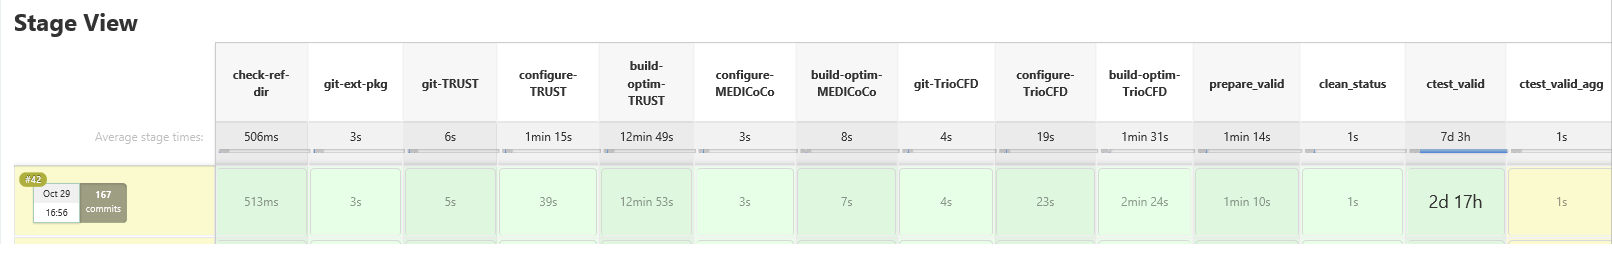
\includegraphics[width=16cm]{pictures/etapes_validation.png}
   \vspace*{0.2cm}
   \captionof{figure}{\label{figure:etapes_validation}Les différentes étapes du processus de Validation de TrioCFD sous Jenkins}
\end{figure}

Une fois le processus arrivé dans l'étape \texttt{ctest\_valid}, l'état de chaque fiche peut être consulté en temps réel dans la page html de suivi qui sera décrite dans la section suivante.

Les résultats de la validation sont stockés dans le répertoire nommé suivant le premier paramètre donné au lancement du Pipeline situé dans \texttt{/volatile/projet/trust\_trio/jenkins/workspace/TrioCFD\_Validation\_pegasi2/validation}. Une fois le processus de validation terminée, le Responsable de code l'archivera dans \texttt{/volatile/projet/trust\_trio/validation/main\_Validation18X/}, répertoire qui comprendra l'ensemble des résultats de validation obtenus entre la version X et X-1 de TrioCFD.


\subsection{Dépouillement des résultats de la base de validation de \texttt{TrioCFD}}

Pour le dépouillement des résultats, le script Groovy \texttt{TrioCFD\_validation.gy} génère une page HTML consultable  depuis l'interface Jenkins, ou pouvant être ouverte par le biais d'un navigateur web lancé depuis la machine où la validation a tourné, à l'adresse : \texttt{/volatile/projet/trust\_trio/jenkins/workspace/TrioCFD\_Validation\_pegasi2/validation/valida\-tion\_label/prm\_report.html}. Cette page est composée de cinq rubriques.\smallskip\\

\begin{minipage}[c]{0.65\linewidth}
La première nommée \textbf{Summary} est un résumé du nombre de fiches ayant tourné avec succès et des fiches en échec. Par échec, on entend à la fois les fiches n'ayant pas abouti et les fiches présentant des écarts avec la version de référence.
\end{minipage} \hfill
\begin{minipage}[c]{0.3\linewidth}
   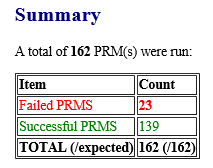
\includegraphics[width=5cm]{pictures/validation-summary.png}\vspace*{0.2cm}
   \captionof{figure}{Dépouillement résultats de validation - partie 1 : Summary}
\end{minipage}
\vspace{0.5cm}

La deuxième nommée \textbf{Running PRMS} liste les fiches de validation en cours de calcul lorsque la page HTML est consultée avant la fin du processus de validation.\vspace{0.6cm}\\


\begin{minipage}[c]{0.5\linewidth}
La rubrique 3, \textbf{Failed PRMS (run failed)}, correspond à un tableau des fiches de validation qui ont planté. Le plantage peut être dû à l'échec d'un des jdds de la fin de validation ou à une erreur lors de la génération du pdf de la fiche.
\end{minipage} \hfill
\begin{minipage}[c]{0.45\linewidth}
   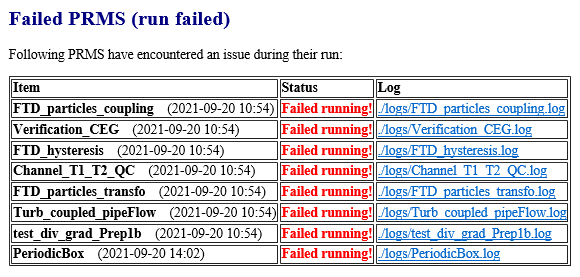
\includegraphics[width=8cm]{pictures/validation-PRMSfailed.png}\vspace*{0.2cm}
   \captionof{figure}{Dépouillement résultats de validation - partie 3 : Failed PRMS}
\vspace{0.6cm}   
\end{minipage}
\vspace{0.6cm}

La quatrième nommée \textbf{Failed PRMS (comparison)} correspond aux fiches ayant tourné avec succès, mais qui présentent des écarts par rapport à la version de référence. Ces écarts sont détectés automatiquement par une comparaison pixel à pixel du nouveau pdf généré et du pdf de la version de référence. C'est alors au Responsable de Code d'intervenir pour faire une analyse manuelle de ces écarts. Ceux-ci peuvent être sans réelle importance et correspondre seulement à un décalage d'une ligne sur le pdf nouvellement généré par rapport à la fois précédente, ou à une légère variation du temps de calcul. A contrario, cet échec de comparaison peut venir d'un impact physique ou numérique important qui devra être justifié ou corrigé.\vspace{0.9cm}   \\

\begin{minipage}[c]{0.25\linewidth}
   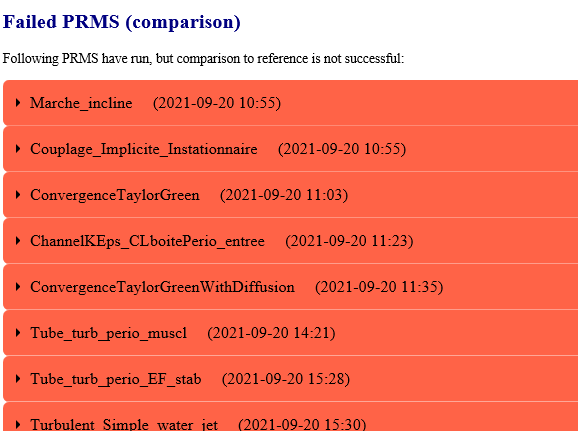
\includegraphics[width=4cm]{pictures/validation-PRMSfailedcomp.png}\vspace*{0.2cm}
   \captionof{figure}{Dépouillement résultats de validation - partie 4 : Failed PRMS au niveau de la comparaison des PDF}
\end{minipage} \hfill
\begin{minipage}[c]{0.7\linewidth}
   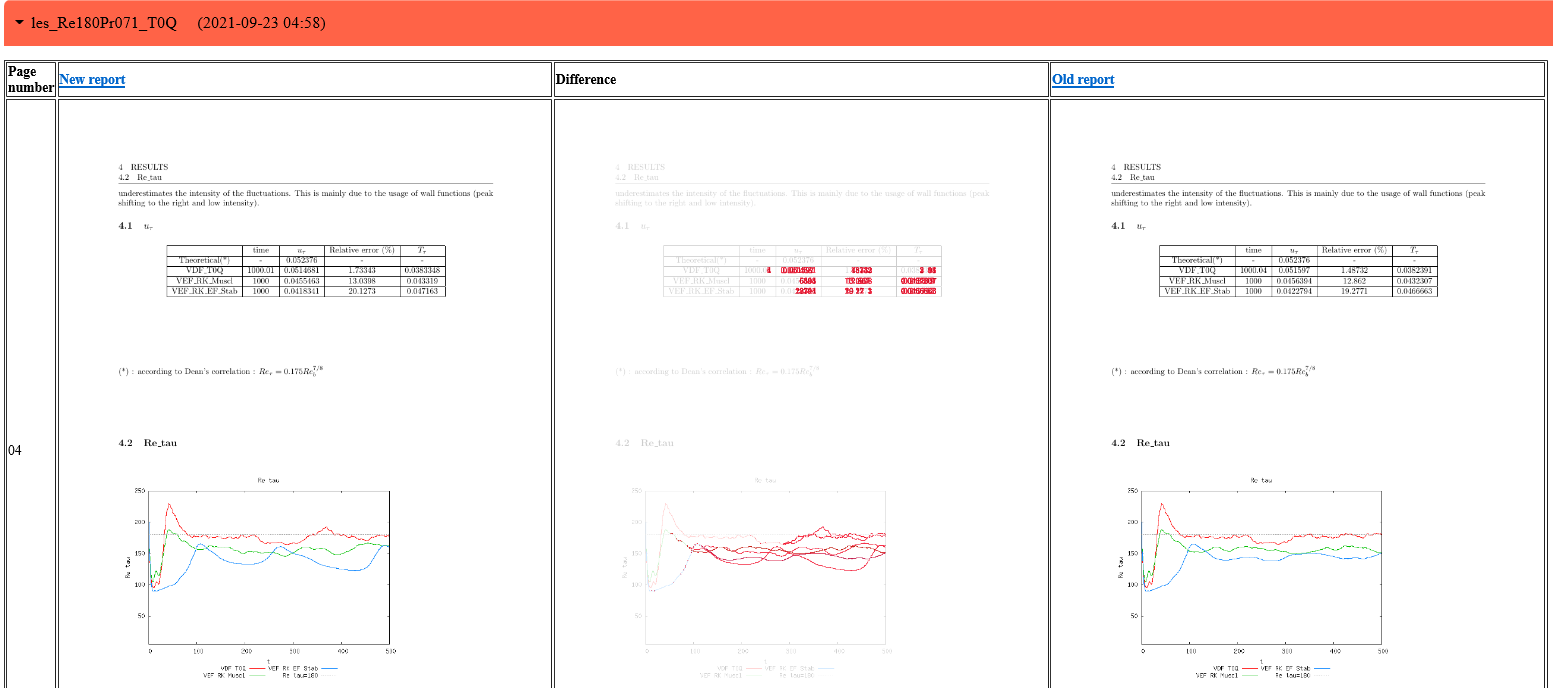
\includegraphics[width=12cm]{pictures/validation-comparepdf2.png}\vspace*{0.2cm}
   \captionof{figure}{Dépouillement résultats de validation - partie 4 : Failed PRMS, exemple de comparaison pixel à pixel}
\end{minipage}
\vspace{0.5cm}

\begin{minipage}[c]{0.5\linewidth}
La dernière partie (\textbf{Successful PRMS} récapitule l'ensemble des fiches de validation qui ont été générées correctement et qui ne présentent aucun écart par rapport à la version de référence.
\end{minipage} \hfill
\begin{minipage}[c]{0.45\linewidth}
   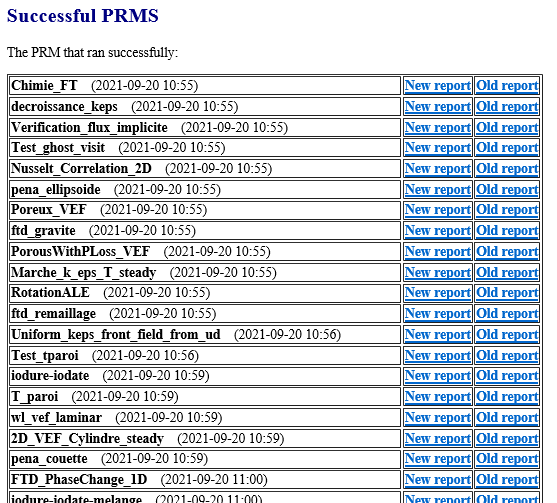
\includegraphics[width=8cm]{pictures/validation-success.png}\vspace*{0.2cm}
   \captionof{figure}{Dépouillement résultats de validation - partie 5 : Successfull PRMS}
\vspace{0.6cm}   
\end{minipage}


%%%%%%%%%%%%%%%%%%%%%%%%%%%%%%%%%%%%%%%%%%%%%%%%%%%%%%%%%%%%%%%%%%%%%%%%%%%%%%%%%%%%%%
\part{\label{partie:doc}Documentation}
\normalsize \normalfont
\rhead{DOCUMENTATION}


\chapter{Appui sur la documentation TRUST}
\lhead{Appui sur la documentation TRUST}
\rhead{DOCUMENTATION}
TrioCFD étant un Baltik de TRUST, toute la documentation de TRUST est applicable pour TrioCFD. Cette documentation de TRUST est disponible soit via la commande \texttt{trust -index} dans un terminal après avoir chargé l'environnement TRUST soit dans le répertoire \texttt{doc/TRUST} de TRUST. Cette documentation est composée de : \\
\begin{itemize}[label=$\Rightarrow$, font=\LARGE]
  \item \textbf{ La Documentation Générale}
  \begin{itemize}
    \item \textit{Release notes} : Elle détaille toutes les intégrations majeures ou les changements ayant un impact sur l'utilisation de TRUST entre deux livraisons de version. Elle est renseignée par le développeur à la fin de son développement/correctif. Pour chacun d'eux, une ligne est ajoutée précisant la date d'intégration dans la version en développement de TRUST, le code sur lequel le travail a eu lieu, la nature de la modification des sources est précisée (New feature, Major Change, Bug fixed,...) et termine par un bref descriptif du travail (figure \ref{figure:RN-TRUST}).\newline
    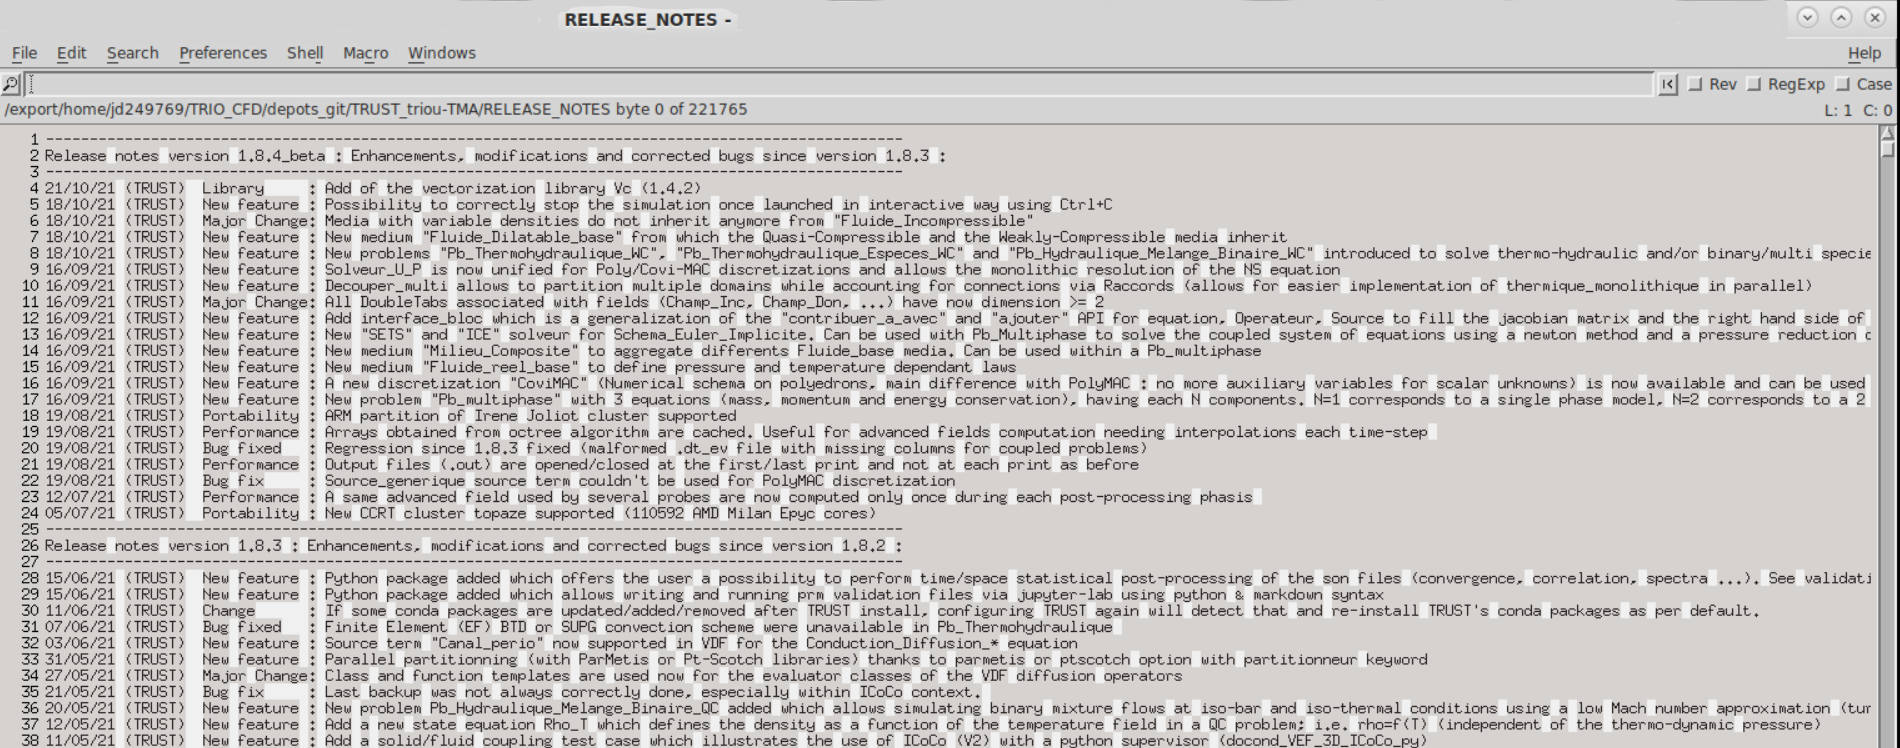
\includegraphics[width=14.5cm]{pictures/RN-TRUST.png}\vspace*{0.1cm}
   \captionof{figure}{\label{figure:RN-TRUST}Release notes de TRUST}
  \end{itemize}
  \begin{itemize}  
    \item \textit{Generic Guide} : Ce guide est le premier document à lire lorsque l'on commence à utiliser la plateforme TRUST. Il présente la plateforme TRUST de façon générale, décrit la méthodologie de lancement des cas-tests, la constitution générale d'un jeu de données, la méthodologie de post-traitement et de lancement d'un calcul en mode parallèle. 
    \item \textit{Reference Manual} : Il est généré automatiquement à partir des balises XDATA présentes dans le code et définies par le développeur. Ce manuel explicite tous les mots clés de TRUST et détaille la façon de les mettre en œuvre dans le jeu de données
    \item \textit{Description note} : Cette note, établie en 2007, présente les différents modèles et équations résolus par Trio\_U puisqu'elle a été émise avant la séparation TRUST/TrioCFD et n'a pas été mise à jour depuis. En ce qui concerne les informations de TrioCFD, celles-ci ne sont pas à prendre en compte dans cette documentation puisqu'une version à jour de ces aspects est présente dans la note spécifique à TrioCFD, nommée \texttt{Description des mod\`eles} (voir section \ref{subsec:modeles}).
    \item \textit{Best practices note} : Tout comme le document précédent, celui-ci, émis en 2013, concerne à la fois TRUST et TrioCFD puisqu'il s'agit d'un guide de bonnes pratiques pour la base de validation de Trio\_U. La partie concernant TrioCFD de cette note a été mise à jour avec la sortie de la documentation spécifique à TrioCFD à savoir le \texttt{Rapport de validation} (voir section \ref{subsec:validation}).
    \item \textit{Validation note} : Cette note émise en 2009 décrit l'organisation de la base de données des cas tests de validation de Trio\_U ainsi que la méthodologie mise en place pour leur automatisation. Comme la note précédente, les informations relevant de TrioCFD ont été mises à jour dans le \texttt{Rapport de validation} (voir section \ref{subsec:validation}).
  \end{itemize}
  \item \textbf{Ressources pour les utilisateurs}
  \begin{itemize}
    \item \textit{User tutorial} : ce tutoriel, à destination des utilisateurs de TRUST et TrioCFD, propose de nombreux exemples et exercices afin de prendre en main l'utilisation de la plateforme. Ce tutoriel est largement utilisé dans la formation utilisateur dispensée par l'équipe TMA.
    \item \textit{Test cases} : tableau récapitulatif des cas tests de référence de TRUST
    \item \textit{Keywords} : tableau de tous les mots clés de TRUST avec lien vers 1 ou plusieurs cas tests utilisant chacun d'eux.
    \item \textit{Memo scripts} : petit mémo des principaux scripts devant être connus par les utilisateurs de TRUST dans leurs prémices sur la plateforme.
  \end{itemize}
  \item \textbf{Ressources pour les développeurs}
  \begin{itemize}
    \item \textit{Developer tutoral} : ce tutoriel, à destination des développeurs de TRUST ou de tout Baltik sous base TRUST, propose de nombreux exemples et exercices afin de prendre en main le codage sur la plateforme. Ce tutoriel est largement utilisé dans la formation développeur dispensée par l'équipe TMA.
    \item \textit{ICoCo tutorial} : ce tutoriel explique la principe de couplage disponible sur la plateforme TRUST grâce à l'outil ICoCo (Interface for Code Coupling), comment le mettre en œuvre sur TRUST et TrioCFD via des exercices et des descriptions de méthodologie pas à pas.
    \item \textit{Other baltik tutorial} : il s'agit d'un document expliquant la création d'un Baltik sous base TRUST. Dans le cadre de TrioCFD, elle est également très utile pour créer des Baltiks ou des sous-Baltiks de TrioCFD, la méthodologie étant la même.
    \item \textit{C++ classes} : documentation DOxygen des classes de TRUST afin d'avoir une vision générale des classes de TRUST, des méthodes rattachées à celles-ci et une description des variables. Elle est générée automatiquement avec la commande \texttt{trust -gui} à partir des balises DOxygen présentes dans le code. Pour les parties de code non balisées, des scripts spécifiques ont été conçus afin qu'elles soient néanmoins prises en compte dans cette documentation indispensable aux développeurs.
    \item \textit{Test coverage} : tableau récapitulatif du nombre de lignes testées dans la partie \texttt{source} de TRUST mais également sur l'ensemble du projet TRUST.
    \item \textit{.prm syntax} : page html expliquant les différents éléments de syntaxe pour la création d'une fiche PRM (fiche de Validation). Si la majorité des mots clés sont applicables à TrioCFD, une nouvelle structure a été mise en place en 2020 dans TrioCFD et les nouveaux mots clés sont décrits dans le rapport de validation de TrioCFD qui sera présenté dans le chapitre suivant.
  \end{itemize}
\end{itemize} 
  
  
\chapter{\label{chapitre:doc-trio}Documentation spécifique à TrioCFD}
\lhead{Documentation spécifique à TrioCFD}
\rhead{DOCUMENTATION}
Outre cette documentation de TRUST, TrioCFD dispose de sa propre documentation en complément. Une grande partie de celle-ci a été mise en place récemment (à partir de 2019) afin de fournir d'avantage de supports à la communauté TrioCFD mais également d'accroître la qualité du code. Jusqu'alors les ressources humaines n'étaient pas suffisantes pour mener de front l'enrichissement des modèles et la mise en qualité. L'ensemble de ces documents sont gérés en gestion de configuration (sous GIT). Ils sont régulièrement enrichis et mis à jour au fur et à mesure des évolutions du code. En effet, leur mise à jour est une étape obligatoire dans tous les processus d'actions menées sur TrioCFD et ils sont relus, au même titre que le code à proprement parler, avant d'être intégrés dans la version. Mise à part la Release Notes qui est un simple document texte, ils sont tous en latex et disposent de leur propre script de génération. Les sources latex de ces documents sont accessibles dans le répertoire \texttt{/share/doc\_src} et disposent d'un répertoire spécifique chacun. Les fichiers PDF correspondants sont, quant à eux, disponibles dans le répertoire \texttt{/share/doc}. Tout comme TRUST, TrioCFD dispose d'une page Html facilitant l'accès à ces différents documents, qui peut être ouverte par la commande \texttt{triocfd -index} après avoir chargé l'environnement TrioCFD.
\subsection{Release Notes}
TrioCFD dispose de sa propre Release notes qui présente la même structure que celle de TRUST : date d'intégration dans le code - code concerné - nature du travail - bref descriptif. Elle présente l'ensemble des modifications/évolutions majeures faites dans le code depuis la version v1.4.0 (mi-2002), version dans laquelle, elle a été mise en place pour la première fois. Elle est organisée par livraison afin que l'utilisateur soit bien informé des changements d'une version à l'autre.\\
Elle est également mise à jour par le développeur lorsque ses travaux font apparaître de nouvelles fonctionnalités dans le code ou modifient le fonctionnement ou les résultats des fonctionnalités existantes. Elle est relue au moment de l'intégration de la branche d'un développement dans le code. Il est recommandé à l'utilisateur de la consulter avant l'utilisation de toute nouvelle version. Des renseignements supplémentaires sur chacun des points peuvent être obtenus auprès de l'équipe de TMA ou du Responsable de Code.
\subsection{TrioCFD Reference Manuel}
Tout comme le Manuel de Reference de TRUST, celui de TrioCFD est généré automatiquement à partir les balises XDATA présentes dans le code et définies par les développeurs pour chaque implémentation de nouveau mot clé. En effet, ce manuel répertorie l'ensemble des mots-clés de TrioCFD à disposition des utilisateurs pour la construction des jeux de données. Il précise la syntaxe exacte à employer pour chacun et décrit brièvement leur utilité.\\
Si ce document n'est pas extrêmement ergonomique et convivial, il présente néanmoins l'intérêt d'avoir les informations sur les mots-clés directement dans le code, ce qui facilite son évolution et sa maintenance. Des travaux sont actuellement en cours afin de mettre en place une documentation des mots-clé plus accessible et riche.
\subsection{Plan de d\'eveloppement TrioCFD 2020-2025}
Sorti en 2019 sous la forme d'une note technique CEA, il a été mis en gestion de configuration début 2021 afin de le mettre à disposition des utilisateurs mais également pour en assurer la sauvegarde.\\
Comme son nom l'indique, il répertorie les développements et les actions de Recherche et Développement prévus dans le code pour la période 2020-2025. Il décrit le programme technique à réaliser et les ressources associées. Il ne concerne que le code de CFD monophasique aux échelles RANS et LES. Les travaux envisagés sur le module de CFD diphasique moyenné, les baltiks FT et IJK font l'objet de documents séparés. Aucune date n'est spécialement définie en face de chaque action. La démarche consiste plutôt à choisir, chaque année, en fonction des sollicitations des utilisateurs et des ressources disponibles, certaines de ces actions et à les traiter. Des développements non définis dans ce document peuvent également être menés afin de répondre aux besoins exprimés par des projets ou des industriels après la rédaction de ce document. Il représente néanmoins la ligne directrice de l'évolution que l'équipe de développeurs CEA souhaite donner au code. D'autre part, il est également possible que certaines actions identifiées à l'époque perdent de leur pertinence au cours du temps et ne soient finalement pas traitées. Finalement, il est à prévoir que certaines actions de R\&D, qui sont longues à réaliser par nature, seront initiées durant cette période et
s'achèveront au-delà de ce terme.
\subsection{\label{subsec:modeles}Description des mod\`eles}
La première version de cette description des modèles est également une note CEA émise en 2019 qui a été mise en gestion de configuration début 2021, en même temps que le document précédent. Cette note décrit les principaux modèles physiques du code de TrioCFD.\\
Dans ce document, la présentation des modèles se concentre
sur la description des écoulements monophasiques, incompressibles, Newtoniens et turbulents. Sa deuxième section rappelle les équations de conservation de masse, quantité de mouvement et d'énergie sont rappelées. Sont également rappelées les définitions des tenseurs de contraintes, de déformation et de rotation qui reviendront dans tout le document. La section se termine par une description des matrices
de masse et de rigidité lorsque le problème de Stokes est discrétisé par la méthode des Volumes-Éléments Finis (VEF). La section suivante présente les différentes approches qui permettent de simuler la
turbulence en LES (Large Eddy Simulations) et en RANS (Reynolds Averaged Navier-Stokes). Pour les modèles RANS, plusieurs modèles de type $\kappa-\epsilon$ sont présentés : le $\kappa-\epsilon$ standard, le $\kappa-\epsilon$ réalisable, et le $\kappa-\epsilon$ bas Reynolds.  Depuis la première version de cette note, le document a été enrichi avec les modèles présents dans les Baltiks Phase\_Field, ALE et Sensitivity\_Analysis. Ce document ne fait, à l'heure actuelle, pas état de l'ensemble de modèles présents dans TrioCFD mais est régulièrement enrichi avec les modèles déjà existants dans TrioCFD et les nouveaux modèles régulièrement développés.
\subsection{\label{subsec:validation}Rapport de validation}
Le rapport de validation a été mis en place fin 2020 et rendu disponible pour la première fois à la livraison de la version v1.8.2. Dès sa création, il a immédiatement été mis en gestion de configuration car il s'agit d'un document évolutif qui fournit aux utilisateurs des exemples d'utilisation de TrioCFD sur les domaines physiques couverts par le code.\\
Il commence par décrire la nouvelle syntaxe des fiches de validation qui a été justement mise en place pour la création de ce document. En effet, jusqu'alors chaque fiche de validation avait sa structure propre définie par son auteur. L'idée a été de mettre en place une structure définie et identique pour toutes les fiches de validation afin de faciliter la lecture et la compréhension de ce rapport. Dans la première version de ce rapport, les fiches de validation couvraient les domaines suivant :\
\begin{itemize}
   \item les écoulements laminaires
   \item les écoulements laminaires avec échanges thermiques
   \item les écoulements turbulents
   \item les écoulements turbulents avec échanges thermiques
   \item les écoulements diphasiques avec le Baltik de Front-Tracking
\end{itemize}
Chaque domaine contient 3 fiches de validation dont les résultats numériques obtenus avec TrioCFD sont comparés soit à l'analytique, soit à des résultats expérimentaux, soit aux résultats numériques obtenus avec d'autres codes. L'entrée d'une fiche de validation dans le rapport de validation nécessite la réécriture de la fiche afin de la mettre au nouveau format. Certaines fiches de validation ne sont également pas suffisamment consistantes pour avoir leur place au sein de ce rapport. Ceci explique pourquoi l'intégralité des fiches de TrioCFD ne figure pas dans ce rapport de validation.
En 2021, trois fiches de validation sur le Baltik ALE, Baltik permettant la modélisation des interactions fluide-structure, y ont été intégrées. Ce rapport sera progressivement enrichi avec de nouvelles fiches dans les domaines existants mais également avec de nouveaux domaines non abordés jusqu'ici.
\subsection{Plan de Gestion de Configuration}
Le PGC ou Plan de Gestion de Configuration de TrioCFD (ce présent document) est le dernier à rejoindre les nouveaux documents mis à disposition des utilisateurs de TrioCFD. Il est disponible, pour la première fois fin 2021 à l'occasion de la sortie de la version v1.8.4. Il a également été immédiatement placé en gestion de configuration, car il s'agit aussi d'un document évolutif qui sera enrichi et mis à jour pour chaque évolution ou modification des pratiques ou des outils du code.


%%%%%%%%%%%%%%%%%%%%%%%%%%%%%%%%%%%%%%%%%%%%%%%%%%%%%%%%%%%%%%%%%%%%%%%%%%%%%%%%%%%%%%
\part{M\'ethodologies et Proc\'edures}
\normalsize \normalfont
\rhead{METHODOLOGIES ET PROCEDURES}

\lettrine[lines=2,slope=0pt,nindent=4pt]{\textbf{A}} chaque type d'action, un processus spécifique est défini afin que celle-ci soit traitée au mieux. On dénombre 4 types différents d'action : développement, étude, demande de maintenance (ayant elle-même plusieurs catégories) et livraison. \\
Chacune a sa propre méthodologie de traitement qui est spécifiée dans cette partie. Le responsable de l'action doit suivre cette méthodologie afin de garantir sa qualité de réalisation et éviter d'oublier certaines étapes cruciales.

\chapter{\label{chapter:dev}Processus de d\'eveloppement}
\lhead{Processus de d\'eveloppement}
\rhead{METHODOLOGIES ET PROCEDURES}
Un développement consiste à introduire un nouveau modèle, une nouvelle fonctionnalité ou nouvel outil dans le code. Le respect d'une méthode de développement (ou bonnes pratiques) a plusieurs avantages :
\begin{itemize}[label=$\Rightarrow$, font=\LARGE]
   \item Elle permet de réduire considérable la dette technique du code. Les coûts ultérieurs, tant pour la maintenance corrective (correction de bugs informatiques) que pour la maintenance évolutive (mise à jour ou ajout de fonctionnalités) peuvent être plus ou moins importants selon la mise en oeuvre de ces bonnes pratiques. Ces coûts additionnels représentent la dette technique d'un logiciel. Une méthodologie de développement permet ainsi de maîtriser les temps de développement mais aussi de réduire la fréquence des bugs.
   \item Elle permet d'accroître la sécurité du logiciel.
   \item Elle permet d'obtenir un code ayant en permanence une bonne qualité jusqu'au moment où une opération de valorisation est envisagée (préparation des audits).
   \item L'application de bonnes pratiques rend propoice le travail en collaboration en établissant un "code de conduite" commun à tous les acteurs.
\end{itemize}

La méthodologie de développement appliquée à TrioCFD va donc être explicitée dans ce chapitre.
\subsection{\label{subsec:specif}Étape 1 : Sp\'ecifications}
Cette étape d'expression du besoin doit être faite en tout premier lieu par le développeur en charge de l'action.
Elle doit couvrir l'intégralité des cas d'utilisation du code,
en expliquant ce qui doit être fait et non pas comment le faire.
Chaque spécification doit pouvoir être testée lors de la dernière phase du développement.
Pendant cette phase de spécification, le développeur doit :
\begin{itemize}[label=$\Rightarrow$, font=\LARGE]
   \item identifier les besoins puis les traduire en termes de fonctionnalités,
         d'interfaces avec les autres modules de TrioCFD, avec TRUST,
         avec les autres Baltiks de TRUST mais également entre elles ;
   \item préciser les enchaînements des actions ;
   \item préciser les contraintes liées au développement (performances, priorités,...) ;
   \item analyser, en fonction des besoins à couvrir, les classes ou modules
         qui pourraient être réutilisés et évaluer les impacts de leur réutilisation sur le développement.
\end{itemize}

Ces spécifications fonctionnelles doivent s'affranchir de la façon dont est implémentée le code.
Il est important de les établir pour ne pas se lancer aveuglément dans le codage.
\newpage
Lors de cette étape, il est pertinent de faire une analyse bibliographique des différents modèles
à disposition pour arriver au besoin ciblé.
Par cette analyse bibliographique, les avantages et inconvénients des différents
modèles pouvant répondre au besoin seront identifiés, de même que leur adéquation
avec la démarche scientifique du code.
Ainsi, le plus pertinent sera plus rapidement identifié.\\
TrioCFD étant un code Open Source, il sera important de s'assurer,
à cette étape, que les choix faits rentrent bien dans cette démarche.\\
En fin de cette étape de spécification, une fiche de Demande d'Intervention
de type \texttt{Maintenance Évolutive} devra être créée dans le BugTracker
et le bilan de cette étape devra y être reporté.

\subsection{Étape 2 : Conception}
Cette étape, également à la charge du développeur,
permet décrire comment le code est censé fonctionner au terme du développement, avant de rentrer dans la phase de codage.
Il s'agit de la réponse technique aux spécialités fonctionnelles faites précédemment.\\
L'activité de conception consiste à :\\
\begin{itemize}[label=$\Rightarrow$, font=\LARGE]
   \item définir le découpage structurel du développement de chacune des
         fonctionnalités identifiées précédemment en classes, méthodes
         et templates puis de détailler chacun d'eux.
         Ce découpage doit respecter les règles de la plateforme TRUST/TrioCFD disponibles dans le \texttt{Developer tutorial} ;
   \item identifier si le développement doit être rattaché à un module existant
         ou si il est nécessaire de créer un nouveau module spécifique ;
   \item identifier la nécessité ou non de modifier ou surcharger des classes de TRUST.
         \textbf{Attention la surcharge de classes de TrioCFD est interdite}.
         Si des classes de TrioCFD ont été identifiées comme pouvant être réutilisées
         dans le cadre du nouveau développement, moyennant certaines adaptations,
         des travaux préparatoires amont devront être menés afin de rendre générique
         cette classe existante puis de créer deux classes filles :
         une pour l'application déjà existante et une nouvelle pour la nouvelle application,
         dérivant de la classe mère;
   \item effectuer l'estimation du temps et des ressources nécessaires pour mener
         à bien les actions de réalisation et de validation afin de prévoir
         son intégration et la validation générale du code associée;
   \item commencer à identifier l'activation de ce nouveau modèle ou application
         dans le jeu de données ainsi que la création des variables de post-traitement
         nécessaires pour mettre en évidence son intérêt et sa validité.
 \end{itemize}
Cette partie architecture (algorithmique) doit être con\c cue en amont de l'écriture du code.
Elle permet de structurer le développement, de séparer ses différentes fonctions
et d'obtenir un codage modulaire et optimisé.
Sans codage modulaire, le développement serait sous forme d'un seul fichier
de plusieurs centaines de lignes de code, le rendant difficile à maintenir et peu évolutif. 

\subsection{Étape 3 : R\'ealisation}
C'est pendant la phase de réalisation à proprement parler que sont réalisés
les développements en vue de répondre aux besoins exprimés lors de la phase de spécification,
en suivant l'architecture définie lors de la phase de conception.
Il est demandé de respecter la découpe architecturale du code
en scindant en plusieurs classes ou fonctions le développement afin d'en améliorer sa maintenance
et sa mutualisation avec d'autres applications.
TrioCFD dispose d'une architecture modulaire avec ses différents modules.
Lors de la phase de codage, il est demandé de poursuivre cette démarche de modularité.\\

Pour rappel, TrioCFD est codé en langage C++ avec une surcharge des classes standard C++ via TRUST.
Il est obligatoire de respecter ce langage.
Aucun fichier source dans un autre langage ne sera intégré dans le code.
En ce qui concerne les procédures, celles-ci sont en Python (3) ou en Bash.
Il n'y a pas d'outil de codage imposé pour mener à bien le développement.
Ainsi, le développeur peut choisir, à sa convenance d'utiliser
soit un éditeur de code classique
soit utiliser un environnement de développement intégré (IDE) type Eclipse ou autre.
Le code doit être explicitement commenté et les messages d'entrées/sorties, clairs et pertinents.
Au niveau de sa racine de TrioCFD, se trouvent 3 répertoires :
\begin{itemize}
   \item le répertoire \textbf{share} : il contient les documents propres TrioCFD dans le sous répertoire \texttt{doc\_src}
         et les rapports de validation propres \`a un module donn\'e dans le sous répertoire \texttt{Validation/\{nomDuModule\}}.
         Ils seront lanc\'es lors du processus de Validation (voir Chapitre \ref{chapitre:validation}).
   \item le répertoire \textbf{src} : il regroupe l'ensemble des fichiers source des modules de TrioCFD (.cpp et .h).
         Si des classes de TRUST sont menées à être surchargées pour un module donn\'e,
         celles-ci seront placées dans un sous-répertoire nommé \texttt{Modif\_TRUST} dans \texttt{src/\{nomDuModule\}}.
   \item le répertoire \textbf{tests} : celui-ci contient l'ensemble des cas-tests de vérification des diff\'erents modules
         et seront lancé lors du processus de Vérification (voir Chapitre \ref{chapitre:verification}).
\end{itemize}

Tout développement devra respecter cet agencement.\\
Les étapes de codage \`a respecter par le développeur sont les suivantes :
\begin{enumerate}
   \item mise à jour du dépôt GIT local de TRUST et TrioCFD dans lequel le développement va être fait ;
   \item création de la branche GIT spécifique au développement
         nommée \texttt{TCFDXXXXXX\_Activité} à partir de la branche de développement
         de TrioCFD nommée \texttt{triou/TMA}.
         Le numéro XXXXXX correspond au numéro d'identification de la fiche relative au développement
         créée dans le BugTracker TrioCFD (voir chapitre \ref{subsec: ficheDI}).
         Il s'agit d'un identifiant unique permettant de faire immédiatement le lien entre chaque
         modification apportée dans le code et sa fiche descriptive associée.
         Le mot \texttt{Activité} va donner un aperçu en 1 mot du sujet sur lequel porte le développement (\textit{eg} Turbulence\_keps, ALE\_vibration,...) ;
   \item codage à proprement parler d'une des fonctionnalités du développement
         général en respectant les quelques recommandations données ci-dessus ;
   \item vérification de la bonne compilation de TrioCFD en mode optimisé et debug ;
   \item définition et implémentation d'un cas-test permettant de vérifier
         la fonctionnalité implémentée avec vérification de son bon fonctionnement ;
   \item commit dans la branche du développement de cette première fonctionnalité
         et push de la branche sur le dépôt GIT distant ;
   \item répétition des étapes 4, 5, 6  et 7 autant de fois que nécessaire suivant
         le nombre de fonctionnalités ajoutées dans le cadre de ce développement.
         Si pertinent, le cas-test pourra être mutualisé pour les différentes fonctionnalités ;
   \item création d'une fiche de Validation (PRM) testant l'ensemble
         du développement pouvant reprendre tout ou partie des cas-tests
         de vérification établis au fur et à mesure ;
   \item lancement de la base de vérification complète de TrioCFD,
         analyse des résultats obtenus, corrections ou justification des écarts si nécessaire ;
   \item documentation du développement qui sera ajouté
         dans un des documents décrits dans la partie \ref{partie:doc} ;
   \item vérification de la bonne compilation TrioCFD en mode optimisé et debug ;
   \item commit des travaux effectués aux étapes 8, 9 et 10 et publication de la branche de développement sur le dépôt distant ;
   \item demande de Pull Request via Tuleap (voir méthodologie expliquée ici \ref{figure:tuleap_PR})
\end{enumerate}

Suite à toutes ces actions, l'étape de codage est terminée et le développement vérifié.
Le développeur doit maintenant mettre à jour la fiche Tuleap de son développement
en expliquant les différents points de commit de celui-ci.
Il y explicite également la possibilité d'impacts physiques ou numériques dans la base de Validation.
En fonction des résultats obtenus lors de la Validation (étape suivante), il est possible que d'autres interventions dans le code soient nécessaires.

\subsection{Étape 4 : Validation}
L'étape suivante consiste à valider ce développement.
Cette étape est à la main du Responsable de Code qui, voyant l'apparition de la demande de Pull Request dans Tuleap
va faire une première relecture du développement et consulter la fiche de BugTracker associée.
En fonction de l'analyse qu'il a mené sur le développement et du message du développeur sur le potentiel impact
de cette branche sur la base de Validation, il lancera ou pas une validation complète.\\
En cas de lancement de la base de Validation à ce moment-là,
le Responsable de Code la lancera à partir du dernier point de commit
de la branche du développement (voir Chapitre \ref{chapitre:validation})
sur la station dédiée à la validation (Pegasi 2) en prenant comme version de référence
la dernière version considérée comme validée.
Cette étape dure environ 60h, durant lesquelles, toutes les fiches de validation sont lancées
et une comparaison pixel à pixel est faite pour chacune.
Les fiches ressortant en écart (les procédures ont détecté des différences de pixel
entre la version de référence et la version à valider) ou en échec
(le rapport PDF de la fiche de validation n'a pas été généré ou un ou plusieurs
cas-tests de la fiche n'a pas tourné) sont analysées par le Responsable de Code.
Dans de nombreux cas, les écarts observés sur les fiches sont en réalité des écarts anodins.
Ces écarts correspondent en réalité à de légères translation de texte ou de figure,
à des arrondis différents au delà de la $5^{ème}$ décimale, à des figures
tracées à quelques centièmes de secondes d'écart par rapport à la version
de référence ou à de légers écarts sur les résultats obtenus ($< à  2 \%$).
Pour ce type d'écarts, le Responsable de Code considère que les résultats de Validation sont corrects.\\
En revanche, lorsque les écarts physiques ou numériques sont significatifs ($> à 2  \%$),
le développeur est sollicité afin d'apporter un avis d'expert sur leur validité ou non.
En cas de non validité, le développement doit être repris pour apporter les corrections adéquates.
Les fiches de validation problématiques ayant été détectées lors du lancement de la base de Validation,
celui-ci s'attachera à les relancer en local, une fois les corrections/adaptations effectuées et s'assurera de leur non-régression.\\
Pour le cas des fiches en échec, il sera également de la responsabilité du développeur
d'apporter les correctifs nécessaires (dans le code en lui-même ou sur la PRM)
afin de la rendre de nouveau fonctionnelle. Ce travail sera mené sur la station personnelle du développeur.\\
Une fois les écarts et échecs résorbés,
le développeur effectue un dernier commit sur sa branche et la pousse sur le dépôt distant.
La base de Validation complète n'est pas relancée à cette étape.

\subsection{\label{subsec:relecture}Étape 5 : Relecture et Int\'egration}
La dernière étape du processus de développement concerne, dans un premier temps,
la relecture de la branche du développement.
Cette étape est extrêmement importante car elle permet d'avoir un code plus lisible,
plus homogène et globalement de meilleure qualité.
Sachant son code relu, l'auteur s'oblige à relire lui-même son propre code avant de faire sa Pull Request.
Il va donc ajouter spontanément des commentaires et faire en sorte que son code
soit le plus compréhensible possible pour que la revue de code se passe bien.
Par ailleurs, un second regard permet de limiter la duplication de code grâce à une
deuxième vision et le relecteur peut alors proposer de réutiliser des parties de code déjà existantes.
Même si le relecteur ne teste pas forcément le code, son point de vue extérieur peut identifier
certains bugs en lisant le code (tel que des cas limites que le développeur aurait pu oublier)
ou des problèmes d'implémentation mais également constater une réponse partielle aux spécifications initiales.
Il peut également suggérer l'ajout de tests unitaires pour des cas qui n'auraient pas été prévus
initialement ou l'enrichissement de la documentation si certains aspects restent flous pour le relecteur.\\
Lors de la revue de code, le relecteur s'assure :
\begin{itemize}
  \item de la bonne dénomination de la branche ;
  \item de la pertinence des points de commit et du commentaire associé ;
  \item du bon respect des règles de codage (non duplication de code,
        dénomination des classes, fonctions et variables, optimisation du code,...) ;
  \item de l'adéquation entre le développement produit et les besoins et spécifications initialement émis ;
  \item de la présence et de la clarté de la documentation ;
  \item de la présence et de la pertinence des cas-tests et de la fiche de validation.
\end{itemize}

En cas d'un soucis sur un de ces aspects, le relecteur et le développeur travailleront
ensemble sur les points controversés afin de converger sur la meilleure solution pour le code.
Les échanges sur la revue de code se font via Tuleap dans le ticket du bug Tracker.
La figure \ref{figure:relecture} est un exemple de relecture d'une branche.
   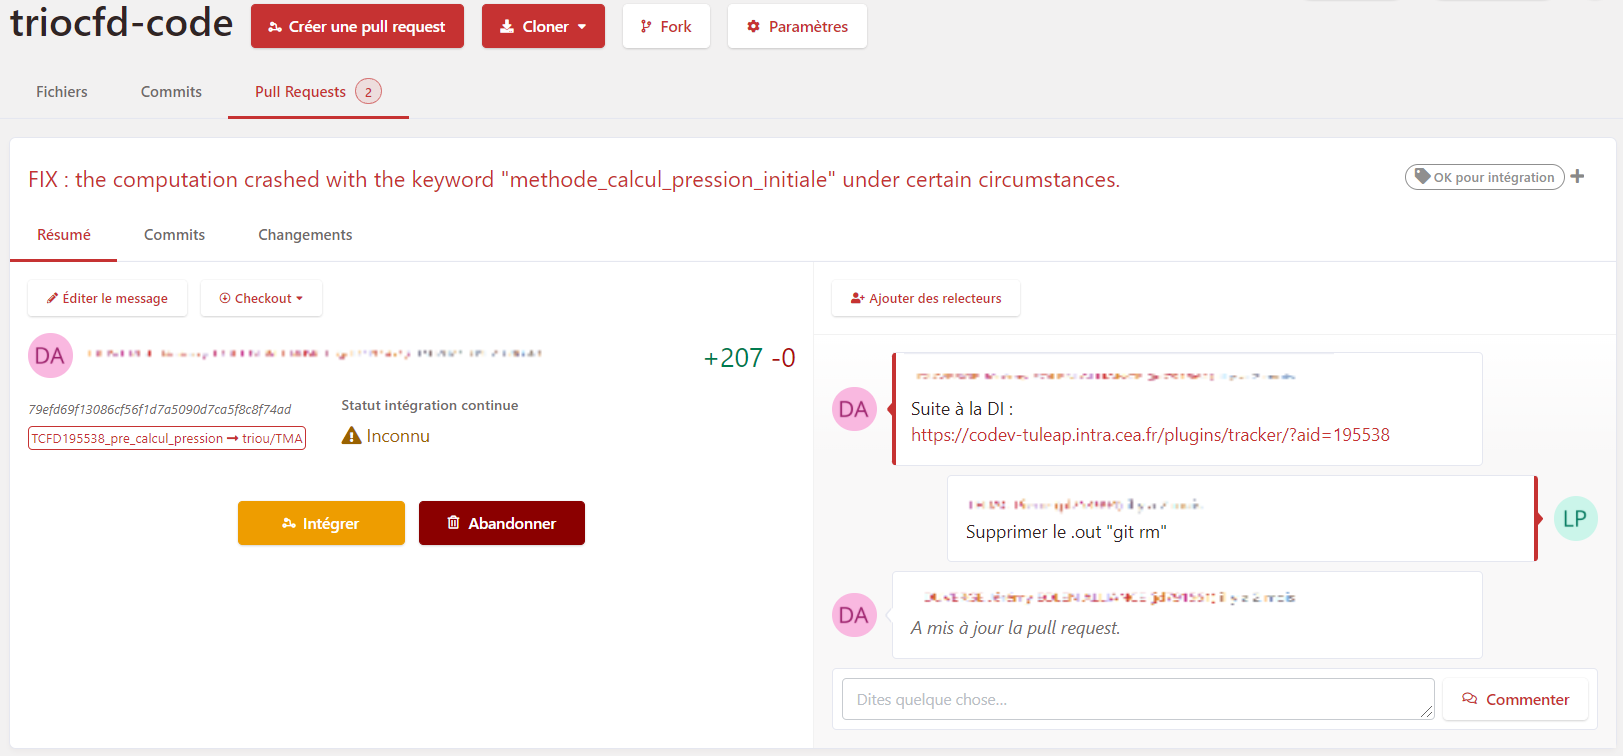
\includegraphics[width=16cm]{pictures/echangesRelecture.png}\vspace*{0.1cm}
   \captionof{figure}{\label{figure:relecture}Exemple d'échange lors de la relecture d'une branche}
\vspace*{0.7cm}   

Suite à la relecture, un commit supplémentaire pourra amené à être
fait sur la branche du développement et la Pull Request, mise à jour.\\

Une fois la revue de code approuvée, le relecteur placera un tag \texttt{OK pour intégration}
(voir figure \ref{figure:relecture} en haut à droite) signifiant que la branche 
du développement a passé avec succès cette étape et peut alors être intégrée dans le code.\\

L'intégrateur intervient alors en rapatriant la branche du développeur dans la branche
de développement de TrioCFD (branche triou/TMA) à date.
La branche de développement ayant pu recevoir d'autres intégrations depuis la création de la branche du développeur,
il vérifie la bonne compilation du code sur la branche de développement avec les nouvelles fonctionnalités
et lance la base de vérification.\\

Si une de ces actions ne donne pas le résultat escompté, l'intégrateur corrigera
la branche de développement avec, potentiellement, l'aide du développeur.
Une fois ces 2 contrôles (compilation + vérification) atteints avec succès,
la branche du développeur est commitée dans la branche triou/TMA et celle-ci est poussée sur le dépôt distant.\\

Les tests de vérification quotidiens tourneront donc, le soir même,
sur cette nouvelle version du code et le statut de la fiche Tuleap associée passera
alors en état \texttt{MERGED} (voir figure \ref{figure:workflow_Trio}).\\

La base de Validation sera lancée sur cette nouvelle version du code le week-end suivant
et lorsque la non-régression sera atteinte, la fiche Tuleap associée sera fermée (statut \texttt{CLOSED}).
L'ensemble du processus de développement sera alors achevé et l'action de développement sera considérée comme terminée.

%\chapter{Processus d'une \'etude}
%\lhead{Processus d'une \'etude}
%\rhead{METHODOLOGIES ET PROCEDURES}
%\vspace{1cm}
%\subsection{Sp\'ecification}\vspace{1cm}
%\subsection{R\'ealisation}\vspace{1cm}
%\subsection{Analyse et Synth\`ese}\vspace{1cm}
%\subsection{Validation}\vspace{1cm}
%\subsection{Archivage}\newpage

\newpage
\chapter{\label{chapitre:livraison}Processus de Livraison}
\lhead{Processus de Livraison}
\rhead{METHODOLOGIES ET PROCEDURES}
La livraison est effectuée conjointement par l'équipe TMA et l'équipe CEA.
Elle commence par la définition exacte de la date de sortie de version.
15 jours avant cette date, l'ensemble des branches (développements et correctifs) doivent avoir
été intégrés dans la branche en développement (\texttt{triou/TMA}).
D'autres intégrations mineures pourront éventuellement avoir lieu ensuite,
notamment en cas d'échec de l'étape de validation de la non-régression.\\
Les étapes importantes qui rythment la livraison sont décrites dans les sections suivantes.

\subsection{Étape 1 : Vérification et Validation de la non-r\'egression}
Une fois l'ensemble des correctifs et développements intégrés dans la version,
la base de vérification tourne une dernière fois sur l'ensemble des machines
du parc afin de s'assurer qu'il n'y ait aucune différence de comportement
entre les différentes configurations couvertes.
L'atelier de génie logiciel est alors désactivé jusqu'à la livraison de la version.\\
La base de validation est lancée une première fois et les non régressions
vis à vis de la dernière exécution de la base de validation sont analysées
afin de maîtriser les éventuels impacts des dernières intégrations
(voir méthodologie décrite au chapitre \ref{chapitre:validation}).
Elle est également lancée en prenant comme version de référence, la dernière version livrée du code.
Les écarts obtenus correspondent à la concaténation de l'ensemble des différences
identifiées lors du lancement hebdomadaire du processus de validation.
Des jdds qui n'ont pas subi d'écarts lors des différentes validations
intermédiaires ne doivent donc pas apparaître à ce moment-là.\\
Une fois ces 2 exécutions complètement analysées et justifiées,
la nouvelle version du code est considérée comme validée.
Les sources du code et les jdds ne devront plus être touchés jusqu'à ce que la livraison soit achevée.

\subsection{Étape 2 : Finalisation de la documentation et dernières intégrations}
L'étape suivante consiste, dans un premier temps, à mettre à jour toute
la documentation afin notamment de faire évoluer le numéro de version,
mais également de faire apparaître l'ensemble des évolutions qui ont eu lieu
dans le code depuis la dernière livraison.
Ceci concerne les documents cités au chapitre \ref{chapitre:doc-trio}.
Une fois l'ensemble de la documentation mise à jour, celle-ci est intégrée dans la branche \texttt{triou/TMA}
et constituera le dernier point de commit.\\

La branche \texttt{master} est alors merg\'ee dans la branche de développement de TrioCFD (\texttt{triou/TMA})
en r\'ealisant une \emph{avance rapide} (\texttt{git merge --ff-only triou\/TMA}).\\
Un tag est apposé avec le nom de la version livrée (\texttt{vx.x.x}).

\subsection{Étape 3 : G\'en\'eration de l'archive et livraison via GitHub}
Vient ensuite l'étape de la mise à disposition aux utilisateurs et développeurs extérieurs au CEA.
La nouvelle version leur est transmise via GITHUB depuis 2021
à l'adresse \url{https://github.com/cea-trust-platform/TrioCFD-code}
(Auparavant, la plateforme utilisée était Sourceforge).
La version est disponible sous GITHUB au format \emph{base git}.
Il contient l'ensemble du code, des jdds et des procédures de TrioCFD
identique au dépôt GIT de TrioCFD hébergé sur Tuleap.
La dernière version livrée correspondra à la branche \texttt{master} du dépôt GITHUB.

\subsection{Étape 4 : Mise \`a disposition sur les Clusters}
Finalement, la nouvelle version sera livrée aux utilisateurs CEA avec son installation
sur l'ensemble des clusters répertoriés (5).
Ils pourront également utiliser la version réseau de cette nouvelle
version disponible sous \texttt{/home/triou}.\\

A l'issue de toutes ces étapes, un mail sera envoyé à la communauté CEA de TrioCFD,
décrivant les évolutions du code depuis la dernière version livrée et
donnant les différents liens pour l'utiliser. Pour la communauté extérieure au CEA,
l'information sera communiquée par le site de TrioCFD (voir chapitre \ref{chapitre:site}).\\

Lorsque toutes ces \'etapes auront \'et\'e r\'ealis\'ees,
les intégrations reprendront dans le code en vue de l'enrichir pour la version suivante.

\chapter{Demande de maintenance}
\lhead{Demande de maintenance}
\rhead{METHODOLOGIES ET PROCEDURES}
Les actions de la TMA sur TrioCFD se font dans le cadre d'un cahier des charges relatif à
la prestation de maintenance informatique des codes de calcul en thermohydraulique.
Ce contrat est commun à différents codes du CEA.\\

Dans le cadre de ce contrat, diverses actions sur le code sont gérées par la TMA avec
un suivi régulier de la part du CEA par le RLP et le Responsable de Code.
Outre les échanges quotidiens, plusieurs réunions contractuelles doivent avoir lieu pour assurer le suivi :\\ 
\begin{itemize}[label=$\Rightarrow$, font=\LARGE]
   \item les \textbf{réunions de suivi hebdomadaires} qui permettent de faire
         un suivi rapproché des actions en cours,
         revoir les priorisations sur le code concerné en cas de besoins urgents des utilisateurs,
         ou échanger sur les difficultés rencontrées lors de la résolution des demandes de maintenance;
   \item les \textbf{COSUIV}, se déroulant de façon mensuel, permettent de faire le même suivi
         que les réunions hebdomadaires mais la priorisation est faite en regard des besoins de l'ensemble
         des codes à la charge de la TMA.
         Ainsi, si une échéance importante est prévue sur un code,
         les actions le concernant seront mises en priorité haute par rapport à celle des autres codes.
         Il se tient en présence du RPL, de l'ensemble des Responsables de Code
         et de l'ensemble de l'équipe TMA et donne lieu à compte-rendu de réunion rédigé par le RML.
   \item les \textbf{COPIL} ont lieu de fa\c con bi-mensuelle et réunit les chargés d'affaire (CEA et TMA),
   les RPL, les Responsables de Code, les RML
   (et éventuellement les Chefs de Laboratoires portant les codes et Chef de Service).
   Les COPIL permettent se s'assurer que les attendus contractuels sont bien
   respectés de part et d'autre.
   Un compte-rendu de réunion trace l'ensemble des constats fait lors du COPIL.
\end{itemize}

Les différentes actions à la charge de la TMA ainsi que leur méthodologie de traitement sont décrites dans ce chapitre.

\subsection{Prise en compte et analyse des demandes}
Toute question arrivant dans la boîte mail \href{mailto:trust@cea.fr}{trust@cea.fr}
est prise en charge par la TMA avec un délai de traitement d'un jour ouvré.
Après une première analyse, une fiche de Demande d'Intervention est créée par
la TMA pour chaque problème rencontré. Cette étape préliminaire d'analyse permet
de lui affecter de catégorie parmi celles détaillées ci-après.
Lors du traitement de la Demande d'Intervention, si il s'avère que la catégorie
n'a pas été correctement identifiée, elle pourra être mise à jour lors de son traitement.\\
La saisie sous forme de fiche de chacun des mails reçus permet de garantir
un bon suivi des difficultés rencontrés et de garantir
une réponse à l'ensemble des sollicitations   re\c cues.

\subsection{Traitement des Assistances Aux Utilisateurs (AAU)}
L'équipe de TMA est souvent sollicitée par les utilisateurs car un de leurs
cas tests n'aboutit pas favorablement. La Demande d'Intervention est alors classée
comme Assistance Aux Utilisateurs. A ce stade, rien ne garantit encore que l'erreur vienne
effectivement d'un problème au niveau de la construction du jdd. Les travaux commenceront
par la modification de plusieurs paramètres, bien connus pour jouer sur la stabilité des
calculs comme le pas de temps, le facsec ou le solveur utilisé.
Si ces premiers tests s'avèrent concluant et permettent d'arriver à une fin propre du calcul,
cela voudra dire que le jdd envoyé nécessitait juste de jouer sur ces paramètres numériques. \\
En cas contraire, si le jdd fourni par l'Initiateur est complexe, on essayera de simplifier
progressivement le jdd afin de mieux cerner l'élément problématique.
Ce procédé de simplification couplé à l'analyse des messages obtenus dans
le fichier de sortie (fichier .err) permettront de simplifier les travaux.
Si le problème relève bien du jdd, l'équipe de TMA sera en mesure d'identifier
rapidement le problème de modélisation que l'utilisateur aurait pu introduire dans ce jdd.
La TMA proposera alors une version fonctionnelle du jdd à l'utilisateur en lui expliquant les modifications effectuées et la raison. Si l'utilisateur est satisfait de ces modifications, la DI passe en statut \texttt{Treated/Resolved} et les travaux sont considérés comme achevés.\\
Parfois, il s'avère que la TMA ne parvienne pas à résoudre le problème
immédiatement car celui-ci ne provient pas du jdd en lui-même, mais relève d'un bug au niveau du code.
La DI sera alors requalifiée dans la catégorie Maintenance Corrective.\\

\subsection{Traitement des Maintenances Correctives (MC)}
Pour rappel, une maintenance corrective est la correction d'anomalies dans les sources du code, dans les outils de maintenance, dans la documentation et dans les jeux de données de la base de test.\\
Une fois la fiche de Demande d'Intervention créée et identifiée dans cette catégorie, les travaux sont initiés sur le jdd fourni par l'Initiateur pour reproduire le problème constaté. Si le jdd fourni est complexe, celui-ci sera simplifié afin de mieux cerner l'élément source de bug dans le jdd. Une fois le problème reproduit sur un cas test élémentaire, les travaux de deboggage débuteront jusqu'à la bonne résolution du jdd fourni. Une fois cette étape atteinte en local, une branche GIT sera créée avec la même dénomination que décrite précédemment (voir la section \ref{subsec:WorkflowGIT}), c'est-à-dire avec le numéro de la DI correspondante sur le BugTracker, contentant l'ensemble des sources modifiées ainsi que le cas test ayant permis sa détection. Le Workflow présenté précédemment sera suivi, jusqu'à la clôture de la DI.\\

\subsection{Traitement des Maintenances Evolutives (ME)}
Toute intervention relevant de la maintenance évolutive sera précisément circonscrite, spécifiée et tracée et représentera au plus un volume de travail estimé à 10 h. jours (estimation validée par le CEA). Les interventions de maintenance évolutive demandant plus que 10 jours et moins de 20 jours de travail sont hors des prestations forfaitaires mais s'inscrivent dans le cadre des prestations sur devis. Les interventions de maintenance évolutive demandant plus de 20 jours de travail seront traitées dans un autre cadre que celui du contrat de TMA. Elles entrent également dans la partie forfaitaire du marché actuel.\\

Une Maintenance Évolutive correspond à une action légère de développement avec une répartition des actions décrites au Chapitre \ref{chapter:dev} de cette partie entre l'équipe CEA et l'équipe TMA. Ce type de Demande d'Intervention se fait par sollicitation du RPL vers l'équipe de TMA. Le RPL commence par créer une fiche de Demande d'Intervention dans le BugTracker TrioCFD. Il y précise, à l'aide l'Initiateur, les spécifications (voir section \ref{subsec:specif}) attendues dans le cadre de l'action.\\

Lors d'un COSUIV, l'action est détaillée par le RPL à l'équipe TMA (plusieurs rebouclages peuvent être faits afin de bien cerner l'action) puis le RML établit un chiffrage pour mener à bien la demande de Maintenance Évolutive. Suite à ce chiffrage, le RPL donne son accord (ou non) pour lancer l'action et précise dans la fiche du BugTracker, l'échéance attendue. Le responsable de l'action dans l'équipe TMA est alors en charge d'effectuer les étapes 2, 3 et 4 précisées dans le Chapitre \ref{chapter:dev} de cette partie, avec un point d'avancée à la fin de chacune avec le RPL. L'Initiateur peut également intervenir à l'étape 4 afin de s'assurer que le développement fournit bien les fonctionnalités et résultats attendus. L'étape 5 de relecture et d'intégration est à la charge du CEA. \\

\subsection{Traitement des DI LIV}
L'équipe de TMA est en charge d'assurer 2 livraisons du code chaque année, généralement une fin juin et la seconde mi-décembre. Dans le cadre du marché actuel, il s'agit d'une action sur bordereau de prix (périmètre et chiffrage associé bien défini). Le CEA définit le planning et les destinataires des livraisons de ses logiciels dans les lettres de cadrage semestrielles. Un déplacement sur le site du client du CEA peut éventuellement être nécessaire. 
La livraison des nouvelles versions est planifi\'ee par le CEA, qui en confie une partie de la pr\'eparation et de l'ex\'ecution \`a l'\'equipe TMA (voir chapitre \ref{chapitre:livraison}).\\

Les t\^aches \`a accomplir comprennent notamment :
\begin{itemize}
    \item La compilation sur diff\'erents OS (une douzaine) ;
    \item Le passage des diff\'erents tests (non r\'egression, v\'erification, ...) ;
    \item La g\'en\'eration de la version, la mise à disposition sur l'outil de partage (GITHUB) ;
    \item La mise \`a jour d'une partie la documentation ; 
    \item L'\'etablissement de la note de version ;
    \item Les installations de la version pour chaque OS sur le r\'eseau interne du CEA et les calculateurs (3 \`a 4) du CCRT.
\end{itemize}


\subsection{Traitement des DI FOR}
Ce type de Demande d'Intervention correspond à la dispense de formation auprès des utilisateurs du code. Elles sont au nombre de 2 par an sur TrioCFD, généralement en Mars et en Octobre. Dans le cadre du marché actuel, il s'agit également d'une action sur bordereau de prix (périmètre et chiffrage associé bien défini). Elles ont lieu sur les sites CEA en région parisienne ou en province dans des locaux prévus à cet effet. La durée des sessions est variable, de 1 à 2 jours suivant les codes et les sujets traités. Le nombre de participants est aussi variable, au maximum 12 par session. Les formations peuvent être dispensées en Français ou en Anglais suivant la demande du CEA. Les formations sont planifiées et organisées par le CEA (présentation dans les lettres de cadrage semestrielles) qui en confie la préparation et l'exécution au titulaire du contrat de TMA. \\

Ce type d'activité est identifié comme DI dans le BugTracker à des fins d'organisation/planification de l'activité de maintenance. La fiche de BugTracker permet également d'assurer le suivi des personnes assistant à la formation. Les tâches incombant à la TMA comprennent la préparation des machines et logiciels de la salle de formation, la préparation/mise à jour des supports de formation et la dispense d'une partie des formations.\\

La formation dispensée sur TrioCFD est une formation à destination des utilisateurs avec, pour commencer, une phase de prise en main puis une description et une démonstration des capacités du code et également de nombreux exercices illustrant les différents domaines et utilisations possibles. Une seconde formation à destination des développeurs est supportée par l'équipe TRUST mais convient également parfaitement aux développeurs de TrioCFD puisque tous deux utilisent le même langage, la même architecture et la même philosophie de codage. Elle dure également 2 jours et nécessite la formation dite "utilisateur" comme pré-requis.\\

En terme de déroulé, le CEA et la TMA commencent par définir la date exacte pour la dispense de la formation, environ 2 mois avant les mois habituels, soit en janvier et en août. Une fois cette date définie, le RPL s'assure de réserver la salle de formation. Un mail d'annonce est  envoyé, dans la foulée, par la TMA aux utilisateurs répertoriés du projet. Toutes les réponses sont archivées dans la fiche correspondante du BugTracker. 1 mois avant la formation, les participants sont sélectionnés par date de réception de leur demande avec un ajustement possible en cas de besoin dûment justifié. La TMA les en informe en rappelant la date et le lieu exacte. 15 jours avant la formation, la TMA installe la dernière version de TRUST et de TrioCFD sur les machines sur lesquelles la formation sera dispensée et fournit les supports au CEA pour relecture et impression. 1 semaine avant la formation, la TMA envoie un dernier mail de rappel aux participants de la session. Durant la formation, l'équipe TMA est en charge de la présentation des supports et de l'encadrement des exercices avec un support de l'équipe CEA. En fin de formation, un questionnaire de satisfaction est fourni aux participants afin de faire évoluer leur contenu si besoin.

%%%%%%%%%%%%%%%%%%%%%%%%%%%%%%%%%%%%%%%%%%%%%%%%%%%%%%%%%%%%%%%%%%%%%%%%%%%%%%%%%%%%%%
\part{\label{partie:com}Communication}
\normalsize \normalfont
\rhead{COMMUNICATION}

\lettrine[lines=2,slope=0pt,nindent=4pt]{\textbf{P}}{lusieurs} canaux de communications ont \'et\'e mis en place progressivement autour de TrioCFD
afin de permettre aux utilisateurs et d\'eveloppeurs de TrioCFD d'\'echanger sur le code, sur les difficult\'es qu'ils rencontrent, d'exprimer
leurs besoins autant en terme de d\'eveloppements que d'outils, mais \'egalement de les informer sur les capacit\'es et \'evolutions de
TrioCFD. Chaque canal est d\'edi\'e \`a un type d'information particulier avec une description de chacun d'eux ci-dessous.

\chapter{\label{chapitre:site}Site TrioCFD}
\lhead{Site TrioCFD}
\rhead{COMMUNICATION}

Le site TrioCFD a \'et\'e construit en 2019 et est accessible \`a l'adresse suivante :
"\url{http://triocfd.cea.fr/Pages/Presentation/TrioCFD_code.aspx}". Il est actuellement construit comme illustr\'e sur
la figure \ref{figure:structure_site_trio}. Les rubriques encadr\'ees en rouge ne sont actuellement pas renseign\'ees
et celles en jaune, sont en cours de r\'edaction. Les rubriques non encadr\'ees sont achev\'ees.\newline

\begin{center}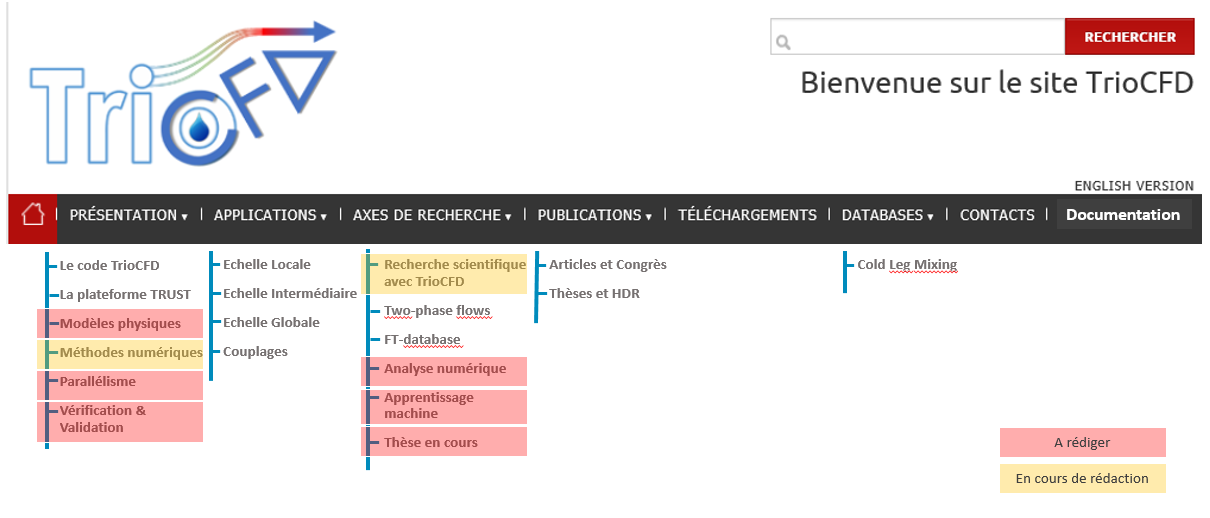
\includegraphics[width=14cm]{pictures/site_Trio.png}\end{center}
\begin{center}\captionof{figure}{\label{figure:structure_site_trio}Structure actuelle du site TrioCFD.}\end{center}

L'objectif du site est de pr\'esenter de fa\c con g\'en\'erale le code TrioCFD, les mod\`eles qui y sont impl\'ement\'es et les applicatifs pour lequel il est utilis\'e/applicable. Un bon nombre d'articles ou de rapport de th\`eses pr\'esentant les travaux effectu\'es avec TrioCFD y sont disponibles ainsi que la documentation du code (rapport de validation, documentation des mod\`eles, manuel de r\'ef\'erence). La page d'accueil regroupe les actualit\'es du code comme l'annonce de s\'eminaire, de sortie de version,... Le lien vers GitHub sur lequel le code source de TrioCFD est disponible est \'egalement r\'ef\'erenc\'e.\newline
Le site s'adresse autant aux utilisateurs interne CEA du code qu'aux utilisateurs universitaires ou industriels. Un formulaire de contact est à la disposition des utilisateurs (pour ceux ne connaissant pas l'adresse du projet) afin qu'ils soient n\'enamoins en mesure de prendre contact avec l'\'equipe en cas de question ou de problème.\newline\\
Pour l'instant, le site est tr\`es majoritairement en fran\c cais et toutes les parties nomm\'ees ci-dessus ne sont pas achev\'ees. Un travail de refonte du site est actuellement en cours afin notamment de l'enrichir avec les nouveaux applicatifs pour lesquels TrioCFD est utilis\'e. Lorsque le nouveau format du site sera termin\'e, celui-ci sera
exclusivement en anglais. Une premi\`ere maquette de la nouvelle structure du site est donn\'ee en figure \ref{figure:nouvelle_structure_site_trio}

\begin{center}
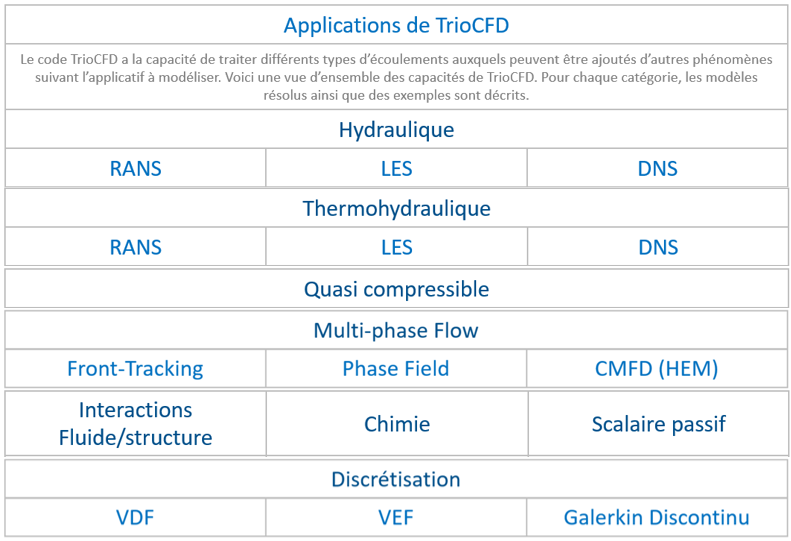
\includegraphics[width=10cm]{pictures/nouveau_site_trio.png}
\end{center}
\begin{center}
\captionof{figure}{\label{figure:nouvelle_structure_site_trio}$1^{\`ere}$ maquette de la nouvelle structure du site TrioCFD.}
\end{center}

Il s'agit l\`a d'une premi\`ere \'ebauche qui pourra \^etre quelque peu modifi\'ee lors de son impl\'ementation. Cette nouvelle structure a pour but de cr\'eer une cartographie compl\`ete et structur\'ee des domaines d'utilisation de TrioCFD, des mod\`eles utilis\'es pour chaque applicatif et des illustrations de ceux-ci par des exemples. Dans sa forme finale, le site pr\'esentera \'egalement l'\'equipe TrioCFD, le formulaire de contact sera conserv\'e ainsi que la base de donn\'ees (\texttt{DATABASE}) et les publications relatives \`a TrioCFD.

\chapter{GT et r\'eunion de d\'eveloppement}
\lhead{GT et r\'eunion de d\'eveloppement}
\rhead{COMMUNICATION}
Deux r\'eunions avec des formats diff\'erents ont lieu chaque mois :
\begin{itemize}[label=$\Rightarrow$, font=\LARGE]
\item \textbf{Groupe de Travail TrioCFD :} il s'agit d'une r\'eunion interne au laboratoire supportant TrioCFD, \`a savoir le LMSF, avec une orientation plut\^ot monophasique ; elle est anim\'ee par le chef de laboratoire. L'\'equipe fait un \'etat d'avancement sur les diff\'erentes t\^aches qui lui sont attribu\'ees sur TrioCFD. Les nouvelles collaborations sont \'egalement pr\'esent\'ees \`a l'ensemble de l'\'equipe avec les enjeux et les difficult\'es rencontr\'ees. Le chef de laboratoire communique \'egalement \`a l'ensemble de l'\'equipe les informations issues de la ligne hiérarchique, et le responsable de lot (SELMA) les informations issues de la ligne projet.
\item \textbf{R\'eunion de d\'eveloppement TrioCFD :} cette r\'eunion est ouverte \`a l'ensemble des utilisateurs et d\'eveloppeurs CEA de TrioCFD (quelque soit son laboratoire ou son site de rattachement) ; elle est anim\'ee par le responsable de code. Celui-ci \'evoque les sujets d'actualit\'e sur TrioCFD (sortie de version, d\'eveloppements en cours ou \`a venir, s\'eminaires,...). Il propose \'egalement \`a l'\'equipe, des outils et pratiques pour am\'eliorer la qualit\'e du code, les conditions de travail pour mener les \'etudes et les d\'eveloppements,... Apr\'es consensus sur ces outils et mise en place, leur utilisation est d\'etaill\'ee dans une r\'eunion de d\'eveloppement suivante.
\end{itemize}

Si un besoin particulier est exprim\'e, une r\'eunion suppl\'ementaire peut \^etre provoqu\'ee, ou la fr\'equence augment\'ee sur une p\'eriode donn\'ee.

\chapter{S\'eminaires}
\lhead{S\'eminaires}
\rhead{COMMUNICATION}

Diff\'erents formats de s\'eminaires rythment l'ann\'ee :
\begin{itemize}[label=$\Rightarrow$, font=\LARGE]
\item \textbf{S\'eminaire des \'etudiants :} Au d\'epart des stagiaires, doctorants ou post-doctorants, un s\'eminaire est organis\'e en interne CEA afin qu'ils pr\'esentent les travaux qui ont \'et\'e effectu\'es dans ce cadre. En ce qui concerne les stagiaires, le s\'eminaire regroupe plusieurs pr\'esentations traitant d'une m\^eme th\'ematique.
Ainsi, plusieurs s\'eminaires de ce type seront organis\'es chaque ann\'ee. Pour les doctorants, le s\'eminaire d\'edi\'e lui permet un entra\^inement en grandeur nature pour sa soutenance de th\`ese.
\item \textbf{S\'eminaire des permanents :} Lorsque un sujet de recherche, une \'etude ou un livrable est arriv\'e \`a maturit\'e, un s\'eminaire sp\'ecifique est organis\'e en interne CEA afin d'\'echanger sur le sujet.
\item \textbf{S\'eminaire TrioCFD :} Tous les 2 ans, le s\'eminaire TrioCFD est organis\'e avec l'ensemble des utilisateurs internes ou externes CEA. La journ\'ee s'articule autour de pr\'esentations techniques autant sur des applications pour lesquelles TrioCFD est utilis\'e pour la mod\'elisation que sur des d\'eveloppements majeurs de nouvelles fonctionnalit\'es. C'est une occasion pour les utilisateurs de d\'ecouvrir les avanc\'ees du code sur les deux derni\`eres ann\'ees et d'avoir un pannel complet des applicatifs. Une partie importante de la journ\'ee est \'egalement d\'edi\'ee aux \'echanges et au partage d'exp\'eriences.
\end{itemize}



%%%%%%%%%%%%%%%%%%%%%%%%%%%%%%%%%%%%%%%%%%%%%%%%%%%%%%%%%%%%%%%%%%%%%%%%%%%%%%%%%%%%%%
\part{Conclusion}
\normalsize \normalfont
\lettrine[lines=2,slope=0pt,nindent=4pt]{\textbf{T}}{his} document
is the first version of a \texttt{TrioCFD} validation report resulting
of an analysis and a sorting work that have been done on its database.
First, an important inventory job was carried out in order to sort
the test cases for targeting quickly the use of \texttt{TrioCFD}
in different CFD configurations. The inventory resulted in a single
table with plenty information (LibreOffice format), where the test
cases are classified into several subdomains of fluid flows. In this
document, some of them have been selected and detailed because 1)
they are well-known in the literature, 2) they present comparisons
with other academic or commercial CFD codes, 3) they present comparisons
with experimental data and 4) they cover an important and representative part of the
physics of the code. In this report, the test cases are representative
of five subdomains: ``Laminar flow'' (Part III), ``Thermal laminar
flow'' (Part IV), ``Turbulent flow'' (Part V), ``Thermal turbulent
flow'' (Part VI), ``Front Tracking'' (Part VII) and "Fluid/structure
interactions with ALE" (Part VIII). The first four
parts gather the test cases for single phase flows, coupled or not with
turbulence models and thermal effects. Part VII is dedicated
to two-phase flows with interface tracking and the last part (VIII) that
has been added since the last version of this report focuses on fluid/structure
interactions with Arbitrary Lagrangian-Eulerian Method (ALE). The corresponding datafiles
were run with the \texttt{1.8.2} version of \texttt{TrioCFD}
to check the achievement of computations. Meanwhile, an important
work was carried out to update a new \texttt{PRM} template in order
to standardize all validation sheets. For each one of them, let us
remind that the PDF file is generated by running a bash script (command
\texttt{Run\_fiche -not\_run}) which acts on a \texttt{PRM} file (previously, test cases must have
been run). A \texttt{PRM} file is a set of specific instructions for interfacing
the \LaTeX ~commands with the \texttt{TrioCFD} results post-processed
with \texttt{Gnuplot} or \texttt{Visit}. Its content can be freely
chosen by authors which has the consequence that the number and titles
of sections differ from one sheet to another one. The goal of the
new \texttt{PRM} template is to harmonize their contents for a more
homogeneous rendering of this report. The seven sections of the new
\texttt{PRM} template detail the main stages of CFD modeling and describe
the comparisons. All validation sheets in this report have been revised
and enhanced by taking into account this new \texttt{PRM} template.

\section*{Perspective}

Numerous other validation sheets already exist in the \texttt{TrioCFD}
database and the job must be pursued. Hence, this document does not
present an exhaustive list of what \texttt{TrioCFD} can do for CFD
applications. It can be viewed as a simple ``snapshot'' that will
be gradually improved and increased at each version release. The improvement
will be simplified by the methodology and the tools which have been
developed for \texttt{PRM} files. After checking and updating the
validations sheets, they will be added in the future versions of this
report. Among the available test cases, the sort will be pursued to
separate those currently ``in progress'' and the others that lack
quantitative comparisons. Multiple variations of the same test case
appear in the database (e.g. ``Poiseuille flow''). Some of them
are simply a 3D extension of the same test case, or an extension with
temperature equation or turbulence model. For instance, the laminar
test case of ``flow with a cylinder'' (Chapter III.3) exists in
turbulent version in two and three dimensions. Another example is
given by the test case named ``Backward facing step'' which appears
in four different versions: the first one is ``two-dimensional'',
the second one is ``implicit'', the third one is ``three-dimensional''
and the last one is ``heated in two dimensions''. More test cases
of turbulent flow are also available, such as ``Baglietto'' and
``Flow in curved pipe''. An effort will be done to extend the
number of CFD subdomains such as ``Quasi-compressible flow'', ``Flow
in porous media'' and ``fluid-structure interaction''. Finally
several tests are dedicated to the ``grid convergence'' or ``Miscellaneous
test'' of numerical options.

%%%%%%%%%%%%%%%%%%%%%%%%%%%%%%%%%%%%%%%%%%%%%%%%%%%%%%%%%%%%%%%%%%%%%%%%%%%%%%%%%%%%%%
%%%%%%%%%%%%%%%%%%%%%%%%%%%%%%%%%%%%%%%%%%%%%%%%%%%%%%%%%%%%%%%%%%%%%%%%%%%%%%%%%%%%%%
\lhead{}
\rhead{BIBLIOGRAPHIE}
\bibliographystyle{plain}
\bibliography{BibTeX_TrioCFD_PGC.bib}
\end{document}
